\documentclass[conference]{IEEEtran}
\usepackage[normalem]{ulem}
\useunder{\uline}{\ul}{}
\usepackage[]{cite}
\renewcommand\citepunct{,}
\ifCLASSINFOpdf
  \usepackage[pdftex]{graphicx}
\else
  % \usepackage[dvips]{graphicx}
  % \graphicspath{{../eps/}}
  % \DeclareGraphicsExtensions{.eps}
\fi
 % 
\usepackage{amsmath}
\usepackage{enumitem}
\usepackage{booktabs}

% *** ALIGNMENT PACKAGES ***
%
\usepackage{array}

% *** SUBFIGURE PACKAGES ***
\ifCLASSOPTIONcompsoc
  \usepackage[caption=false,font=normalsize,labelfont=sf,textfont=sf]{subfig}
\else
  \usepackage[caption=false,font=footnotesize]{subfig}
\fi
% subfig.sty, written by Steven Douglas Cochran, is the modern replacement

 \usepackage{dblfloatfix}

% correct bad hyphenation here
\hyphenation{op-tical net-works semi-conduc-tor}

\begin{document}
\graphicspath{{./images/}}
%
% paper title
% Titles are generally capitalized except for words such as a, an, and, as,
% at, but, by, for, in, nor, of, on, or, the, to and up, which are usually
% not capitalized unless they are the first or last word of the title.
% Linebreaks \\ can be used within to get better formatting as desired.
% Do not put math or special symbols in the title.
\title{Supporting Information \\ {\large High-Throughput Structural Modeling of the HIV Transmission Bottleneck}}

% author names and affiliations
% use a multiple column layout for up to three different
% affiliations
\author{
\IEEEauthorblockN{Scott P. Morton}
\IEEEauthorblockA{spm3c@mtmail.mtsu.edu\\
Center for Computational Science\\
College of Basic and Applied Sciences\\
Middle Tennessee State University\\
Murfreesboro, TN 37130, USA
}
\and
\IEEEauthorblockN{Julie B. Phillips}
\IEEEauthorblockA{jphillips@cumberland.edu\\
Department of Biology\\
Cumberland University\\
Lebanon, TN 37087, USA
}
\and
\IEEEauthorblockN{Joshua L. Phillips*}
\IEEEauthorblockA{Joshua.Phillips@mtsu.edu\\
	Department of Computer Science\\
	College of Basic and Applied Sciences\\
	Middle Tennessee State University\\
	Murfreesboro, TN 37130, USA
}
}

% make the title area
\maketitle

% As a general rule, do not put math, special symbols or citations
% in the abstract

% For peer review papers, you can put extra information on the cover
% page as needed:
% \ifCLASSOPTIONpeerreview
% \begin{center} \bfseries EDICS Category: 3-BBND \end{center}
% \fi
%
% For peerreview papers, this IEEEtran command inserts a page break and
% creates the second title. It will be ignored for other modes.
\IEEEpeerreviewmaketitle

\section{Selection of Principal Components}
Much like a photograph, dimensionality reduction through PCA results in the attenuation of component data. Take a ray in three dimensional space at a $45$ degree angle between the x-axis and the z-axis and a $90$ degree angle from y-axis to the x-axis with has euclidean length of $2$.   This is an overly simplified example for the purposes of demonstration, none the less suitable for our proposed explanation. Projecting this particular ray onto a two dimensional Cartesian Plane can be performed using basic trigonometric calculations. We can determine the projection of the ray onto the x-axis by ignoring the y-axis coordinates altogether due to the angle. This leaves us with the simple Pythagorean theorem of $A^2 + B^2 = C^2$. Knowing the length of the ray (C) we can transpose the problem down to the $sqrt(2)$ leaving us with $1.414$ as the length of the projection onto the x-axis. This equates to a $29.3\%$ reduction of the original ray length. Applying this to the addition of Principal Components in a Cosine Similarity Analysis where each target and source PCA set is compared to the $n^{th}$ PC in a CSA and the data are then averaged out, results in a similar reduction of information. We demonstrate this by displaying the graphs of the ordered sets with inclusions of the first through the tenth PC noting the loss of significant vector lengths as more principal components are added into the process. For this reason we have fixed our choice of principal components at the first $2$.

\begin{figure}
	\centering
	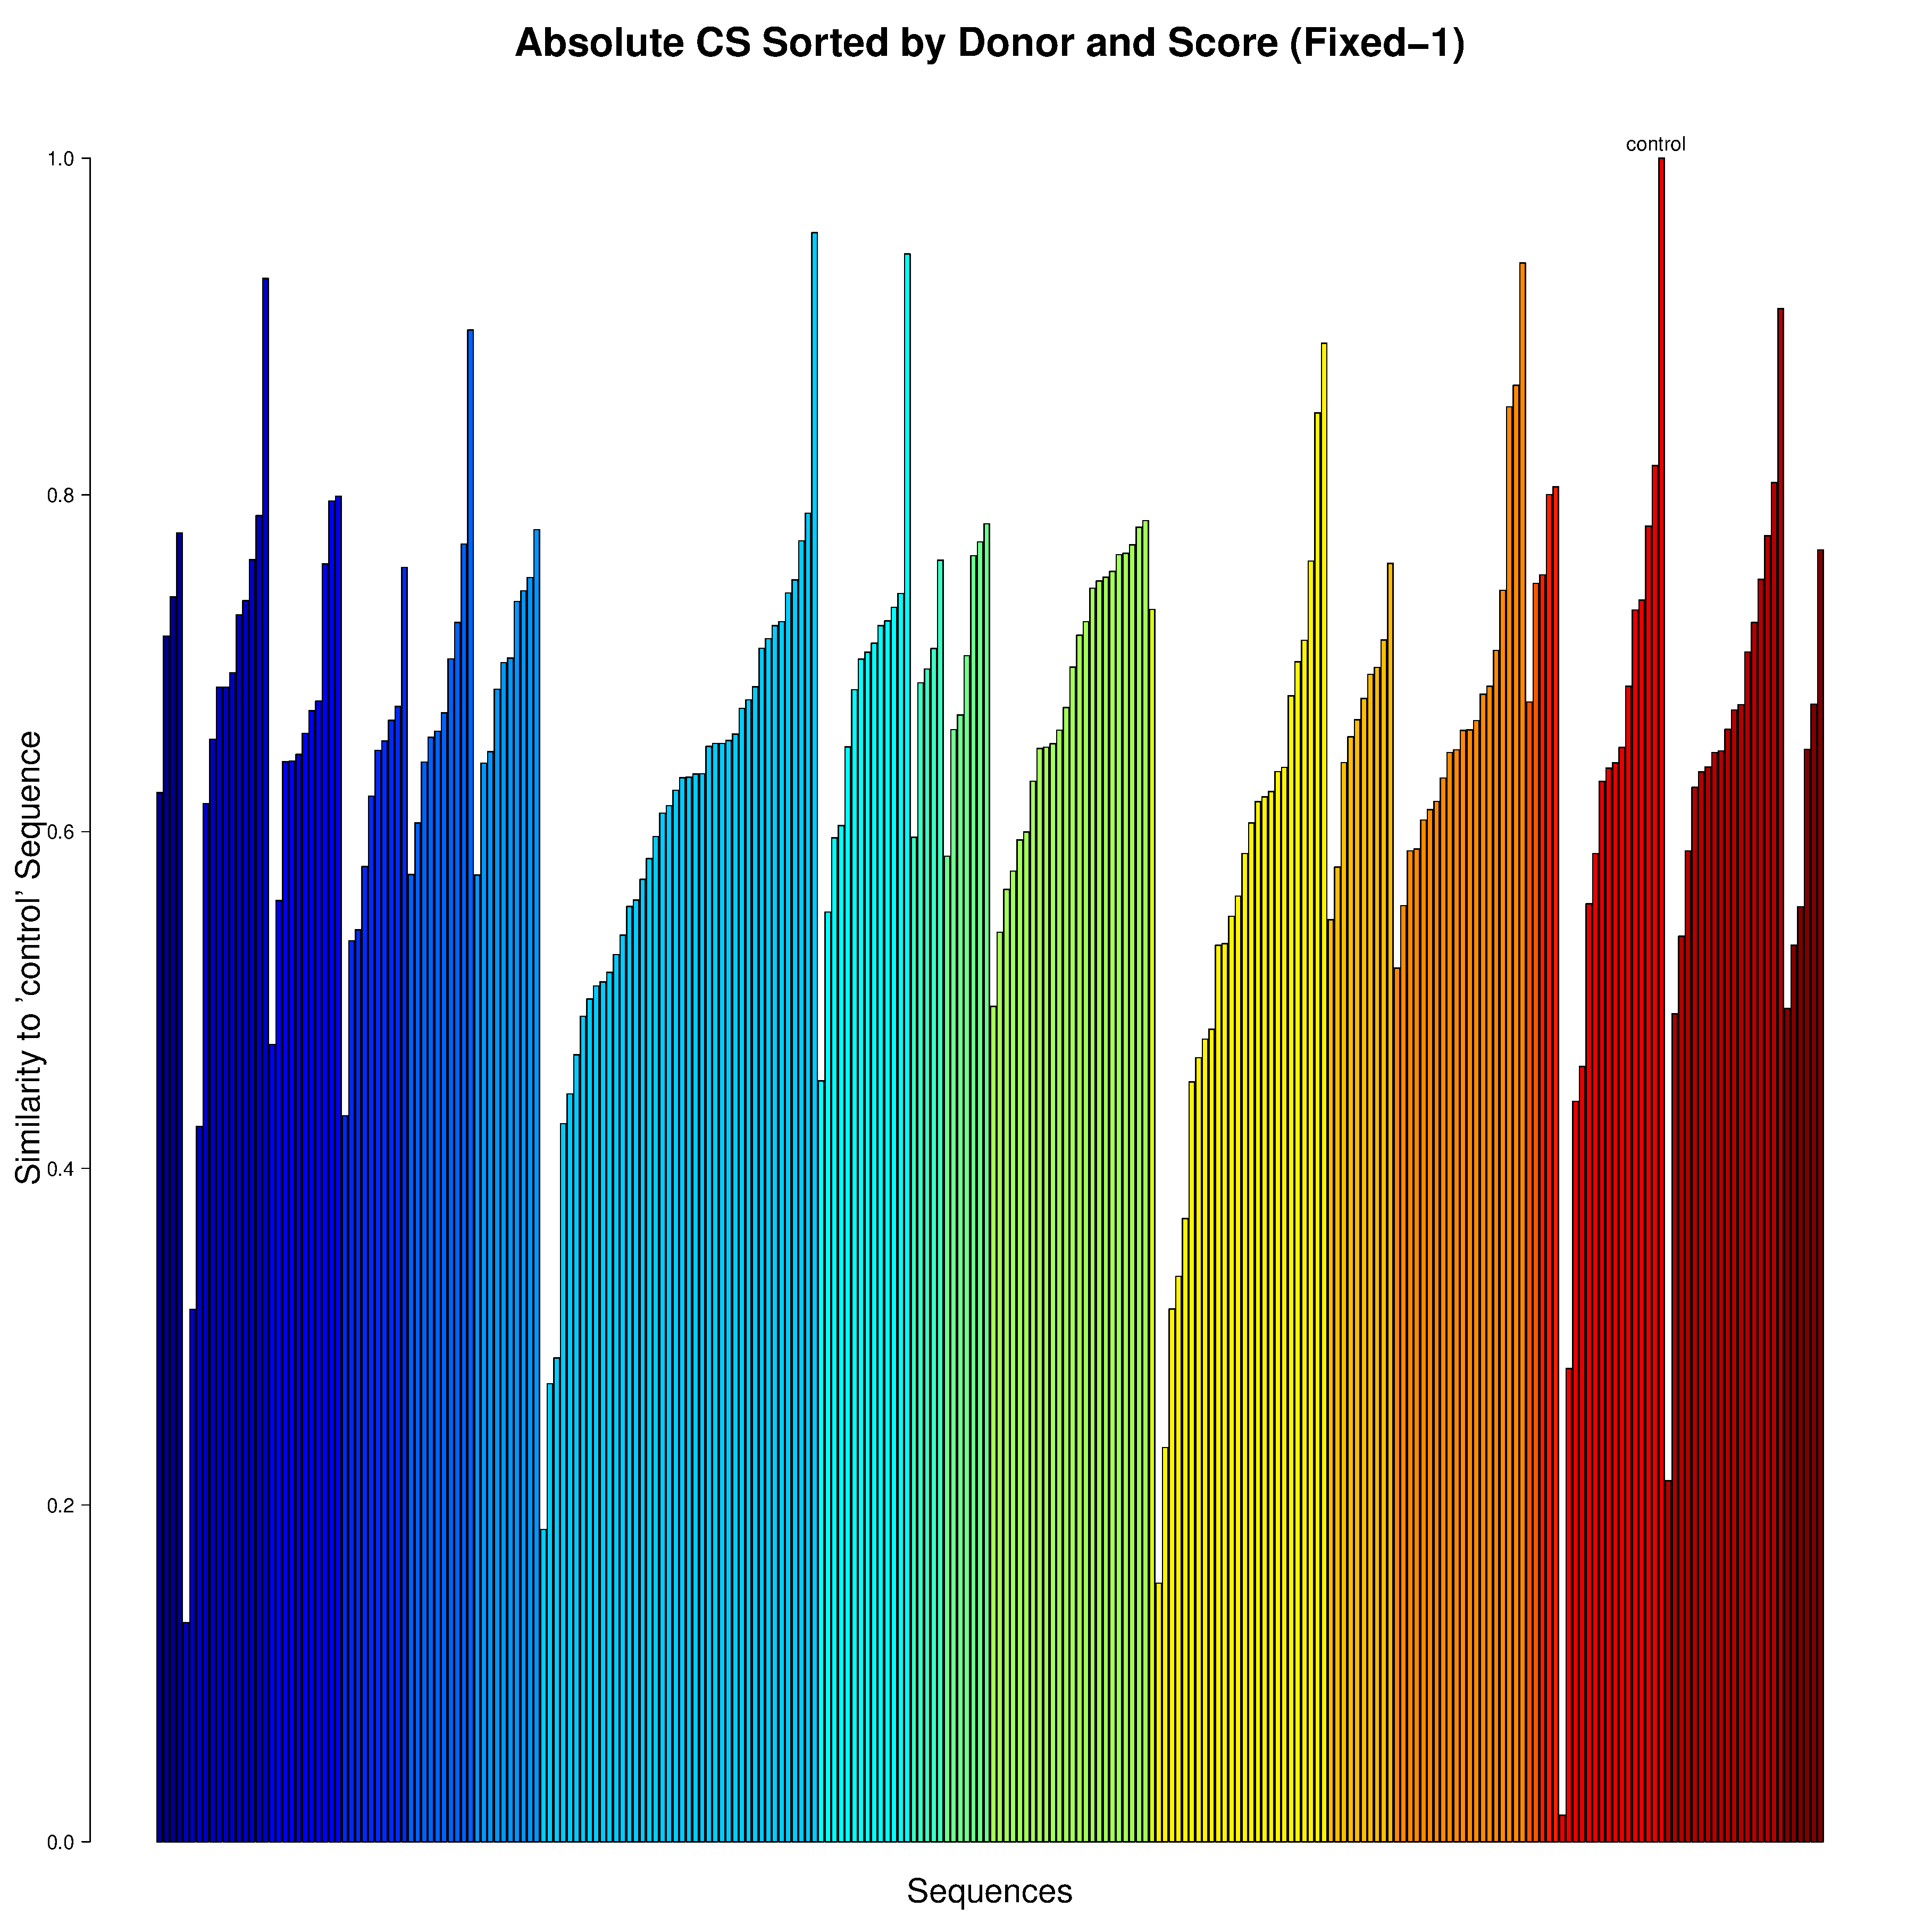
\includegraphics[width=0.8\linewidth]{ordered_by_Donor-Score_PC_Fixed-1}
	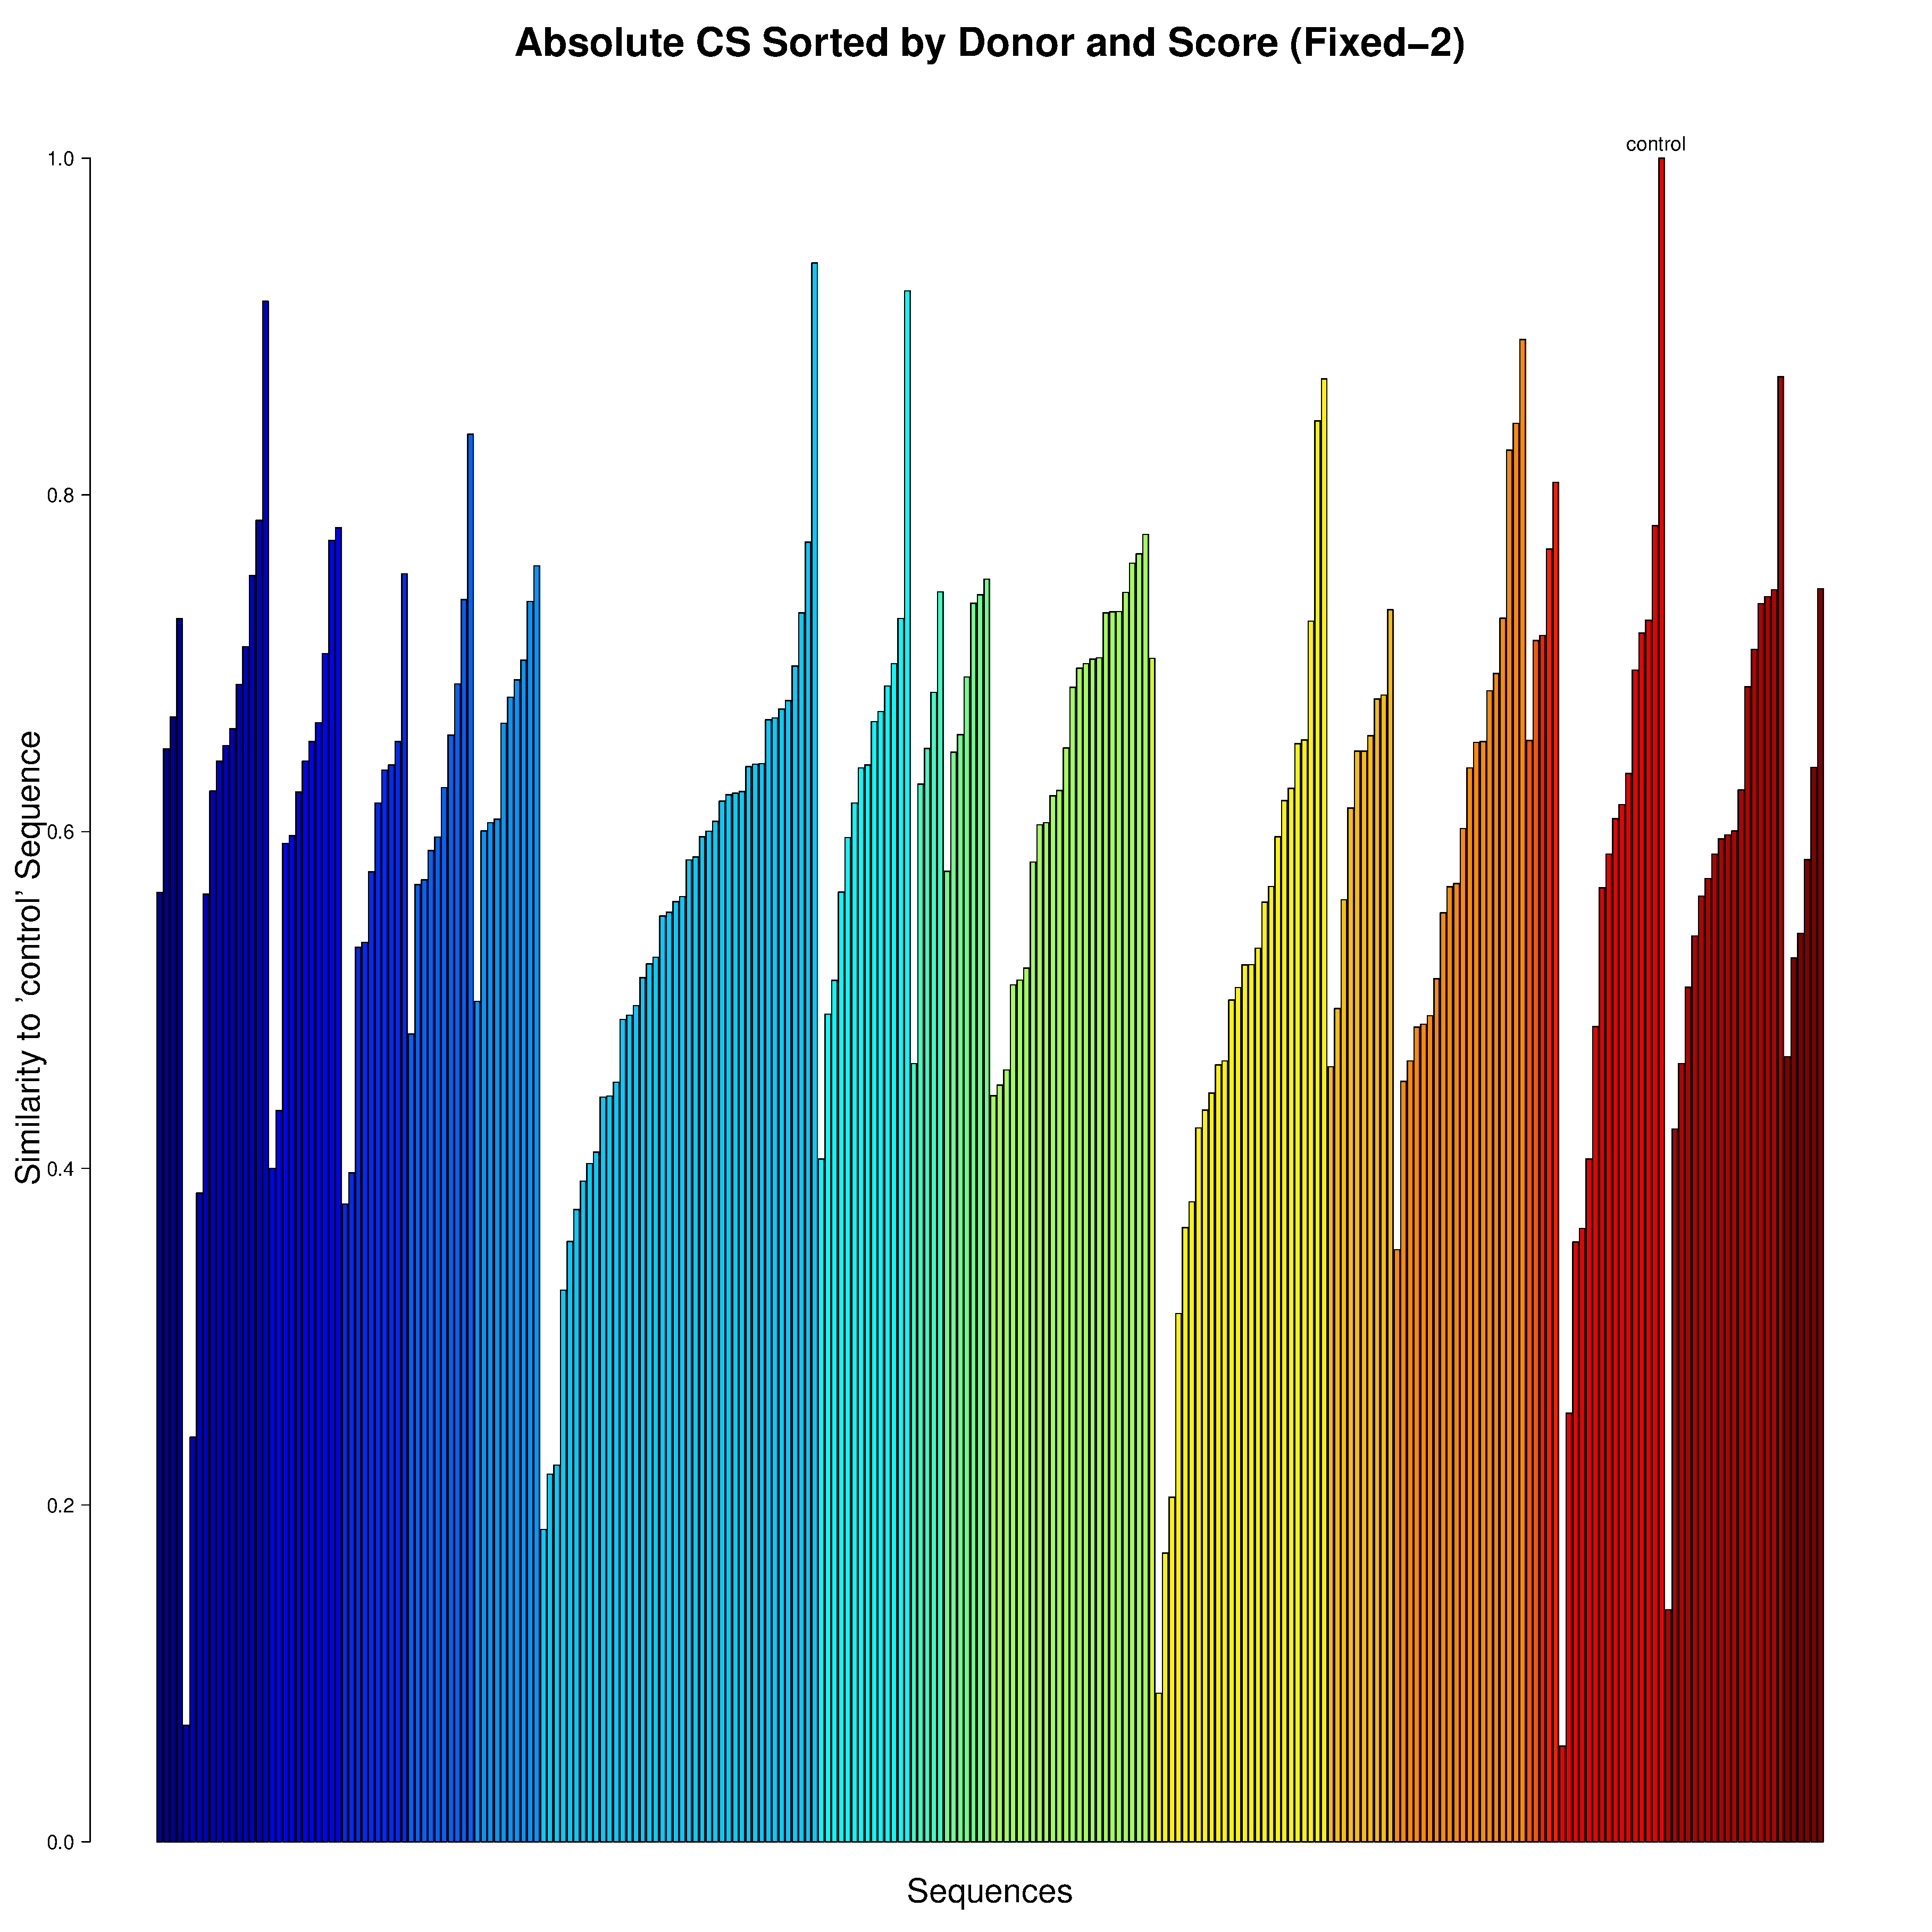
\includegraphics[width=0.8\linewidth]{ordered_by_Donor-Score_PC_Fixed-2}
\end{figure}
\begin{figure*}
	\centering
	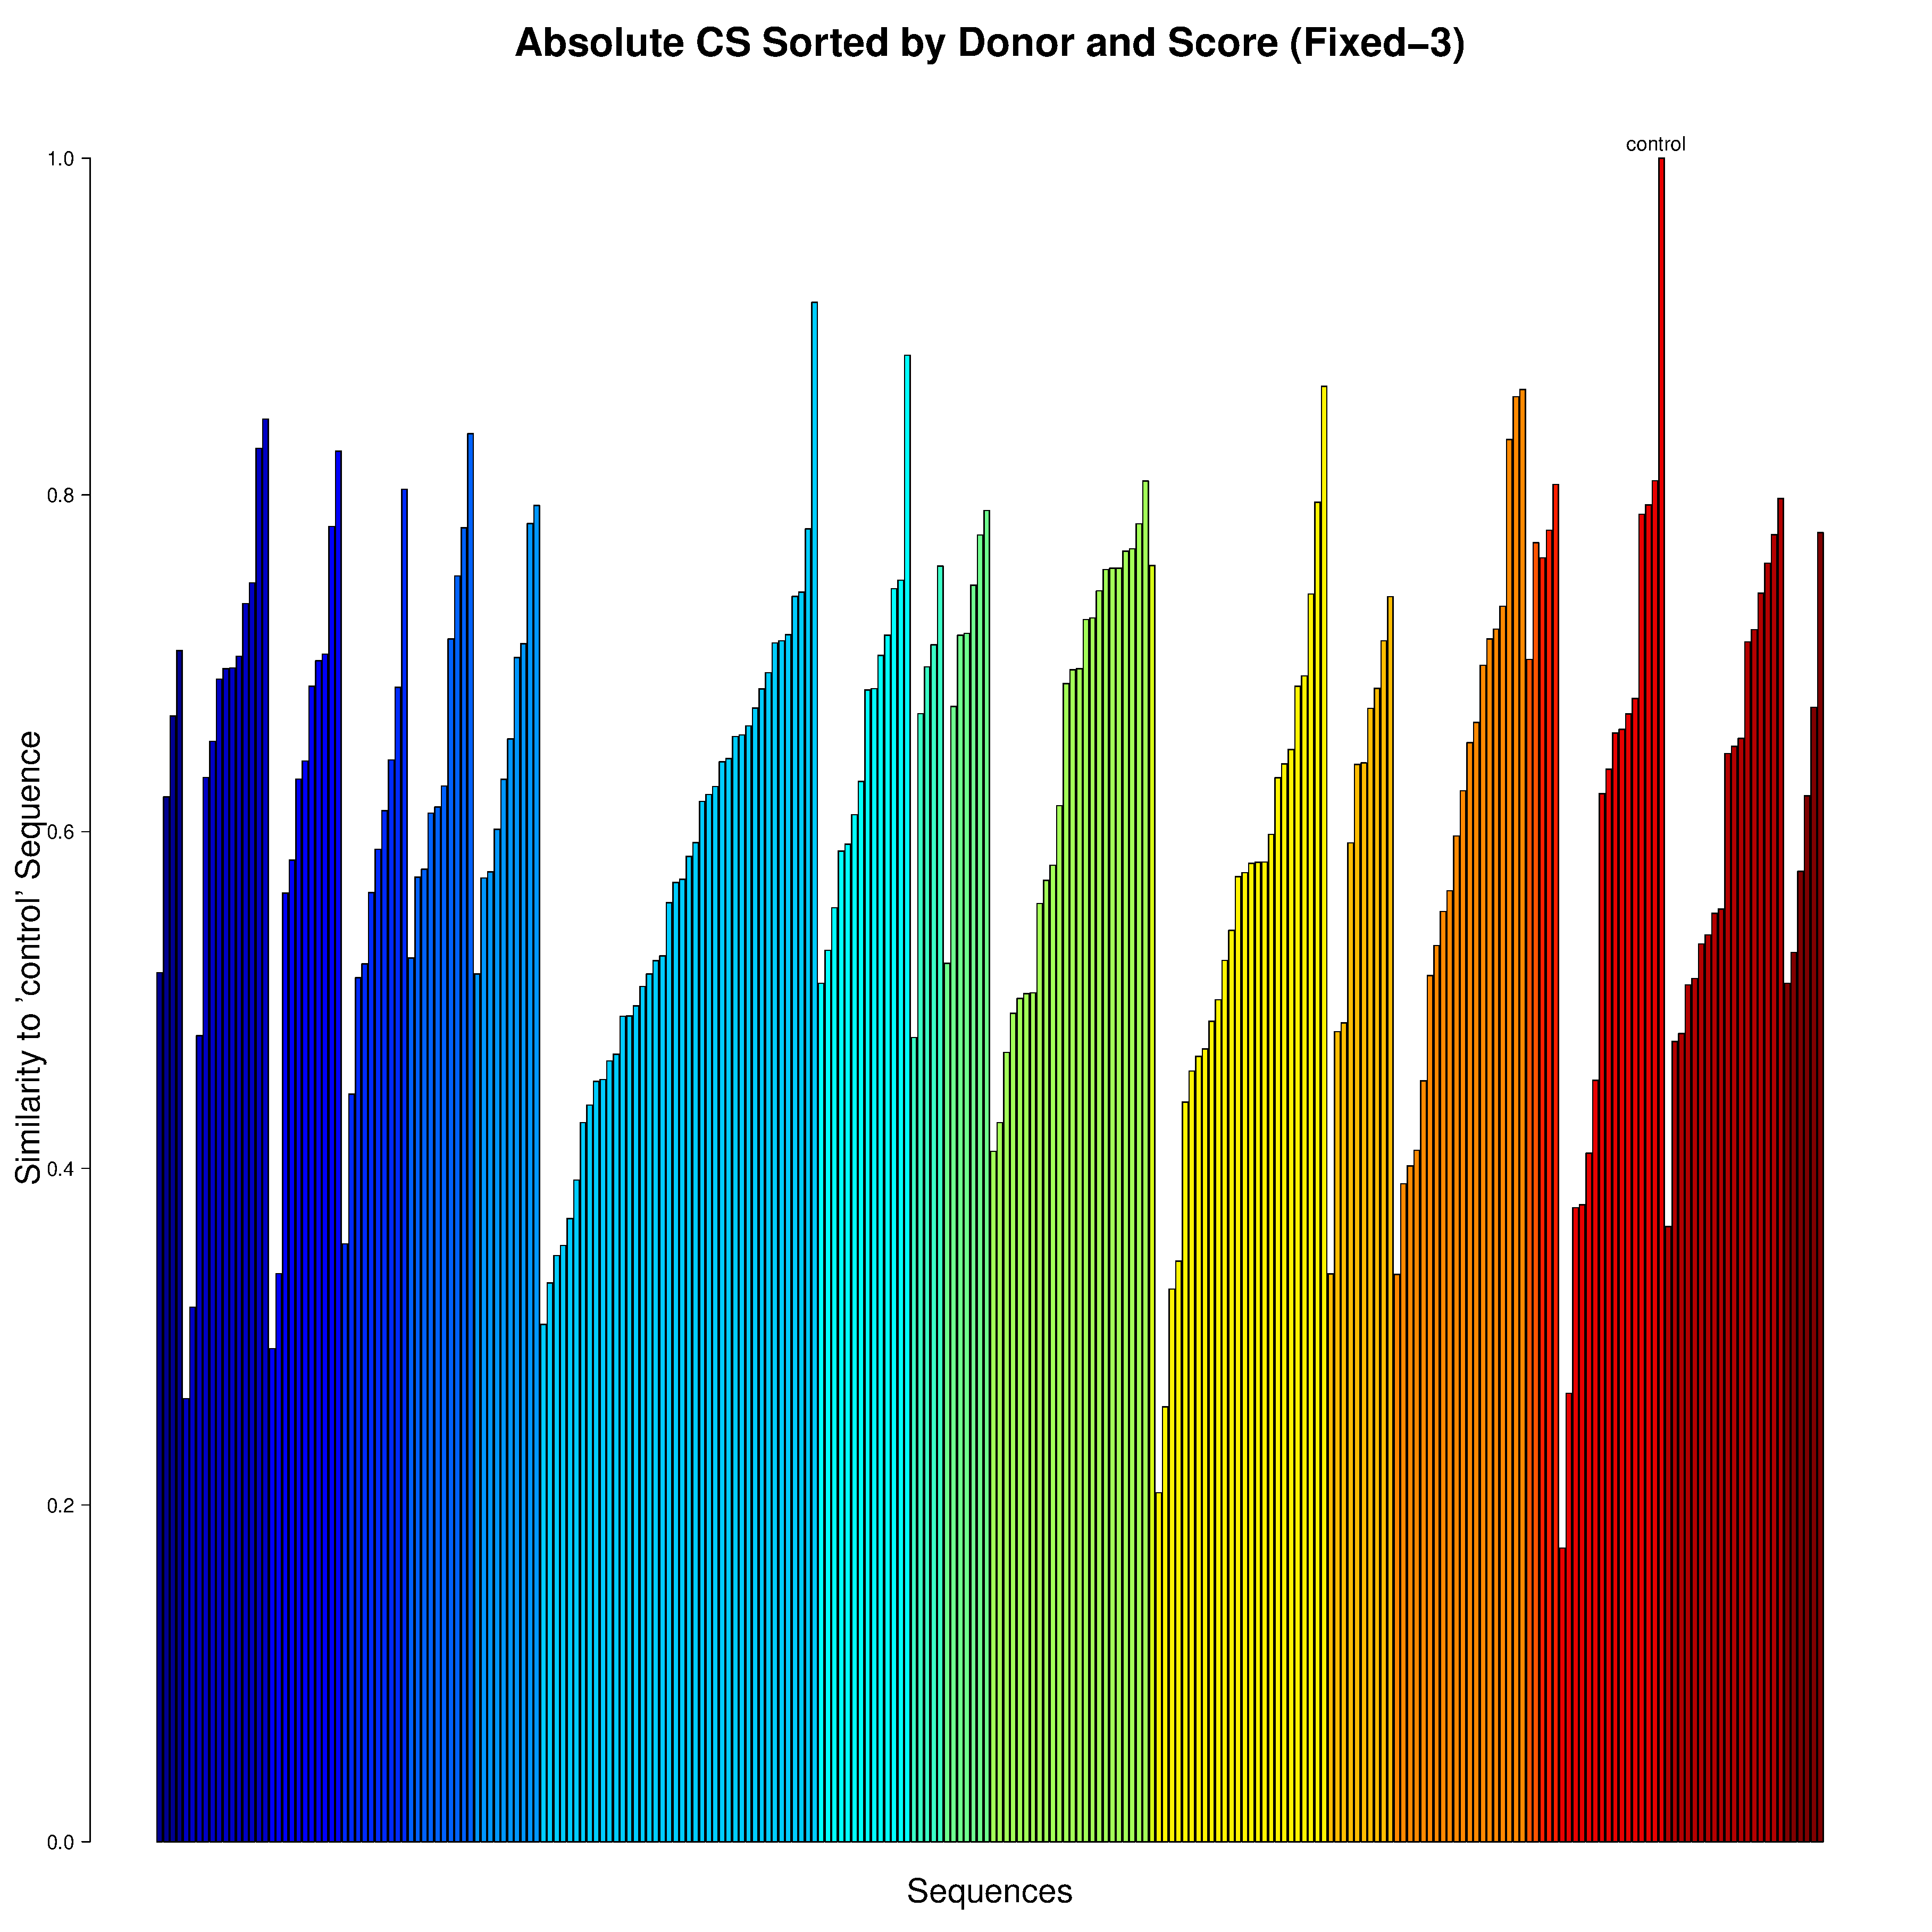
\includegraphics[width=0.4\linewidth]{ordered_by_Donor-Score_PC_Fixed-3}
	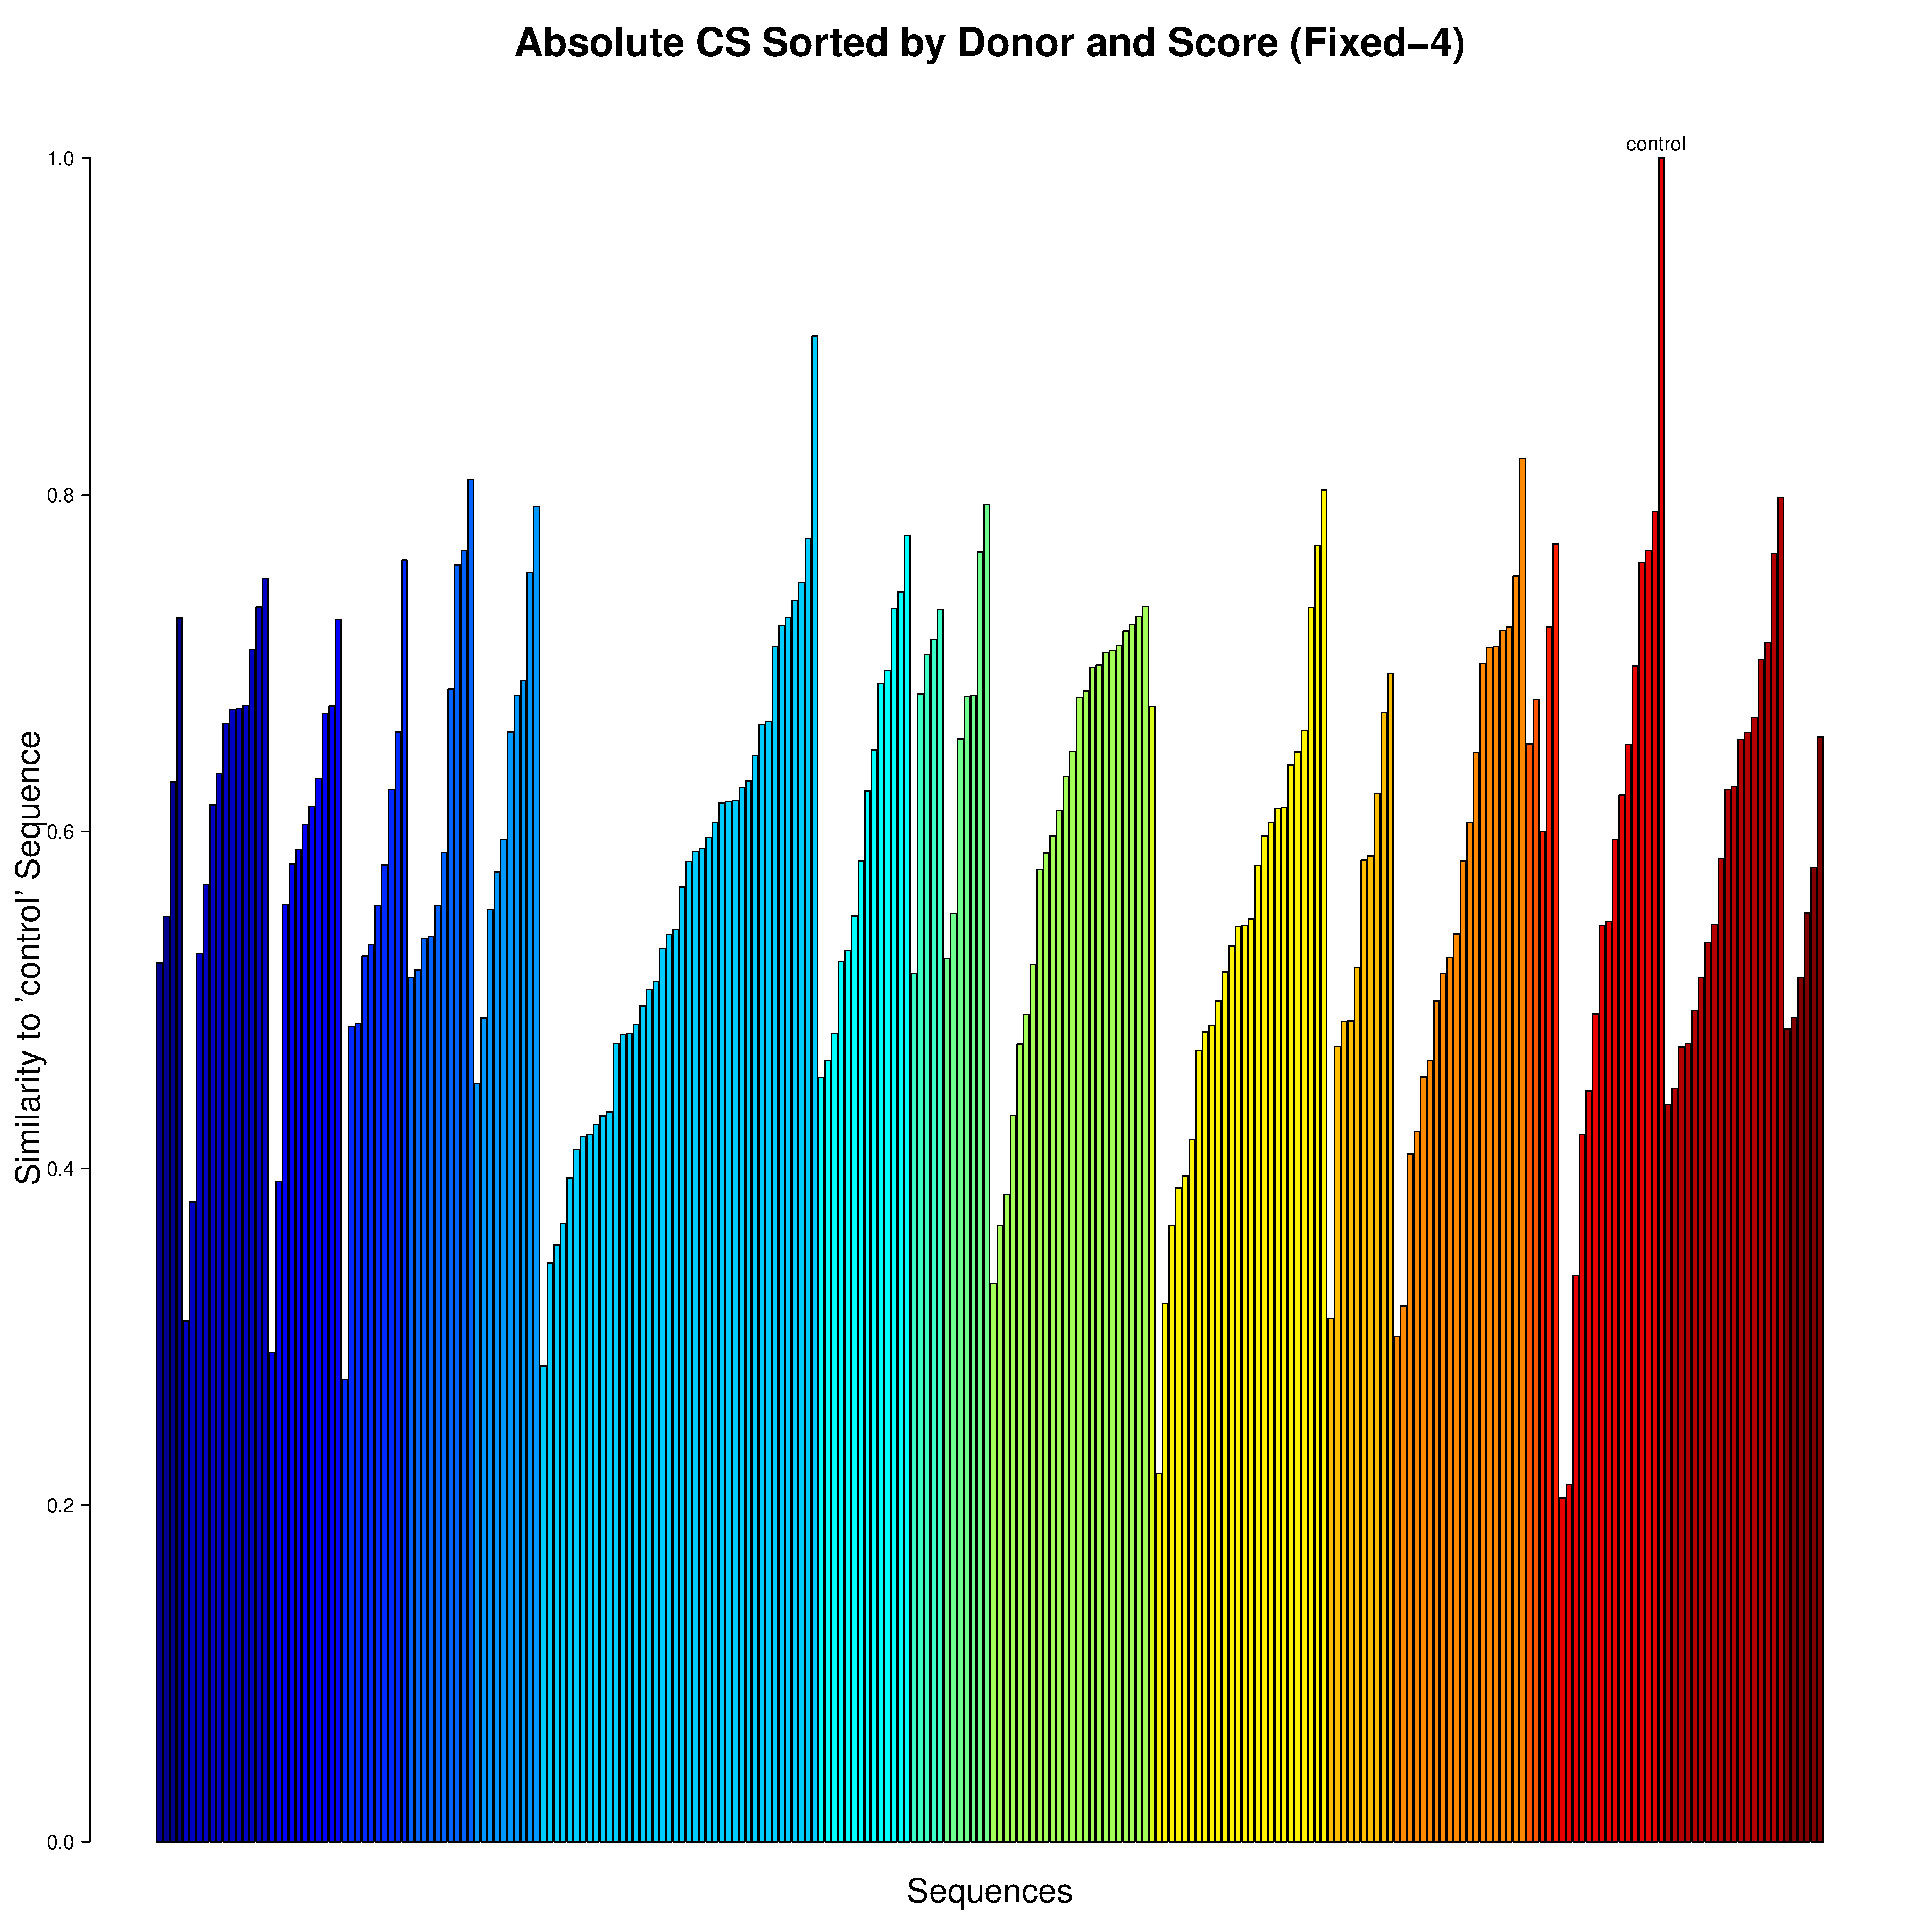
\includegraphics[width=0.4\linewidth]{ordered_by_Donor-Score_PC_Fixed-4}
\end{figure*}
\begin{figure*}
	\centering
	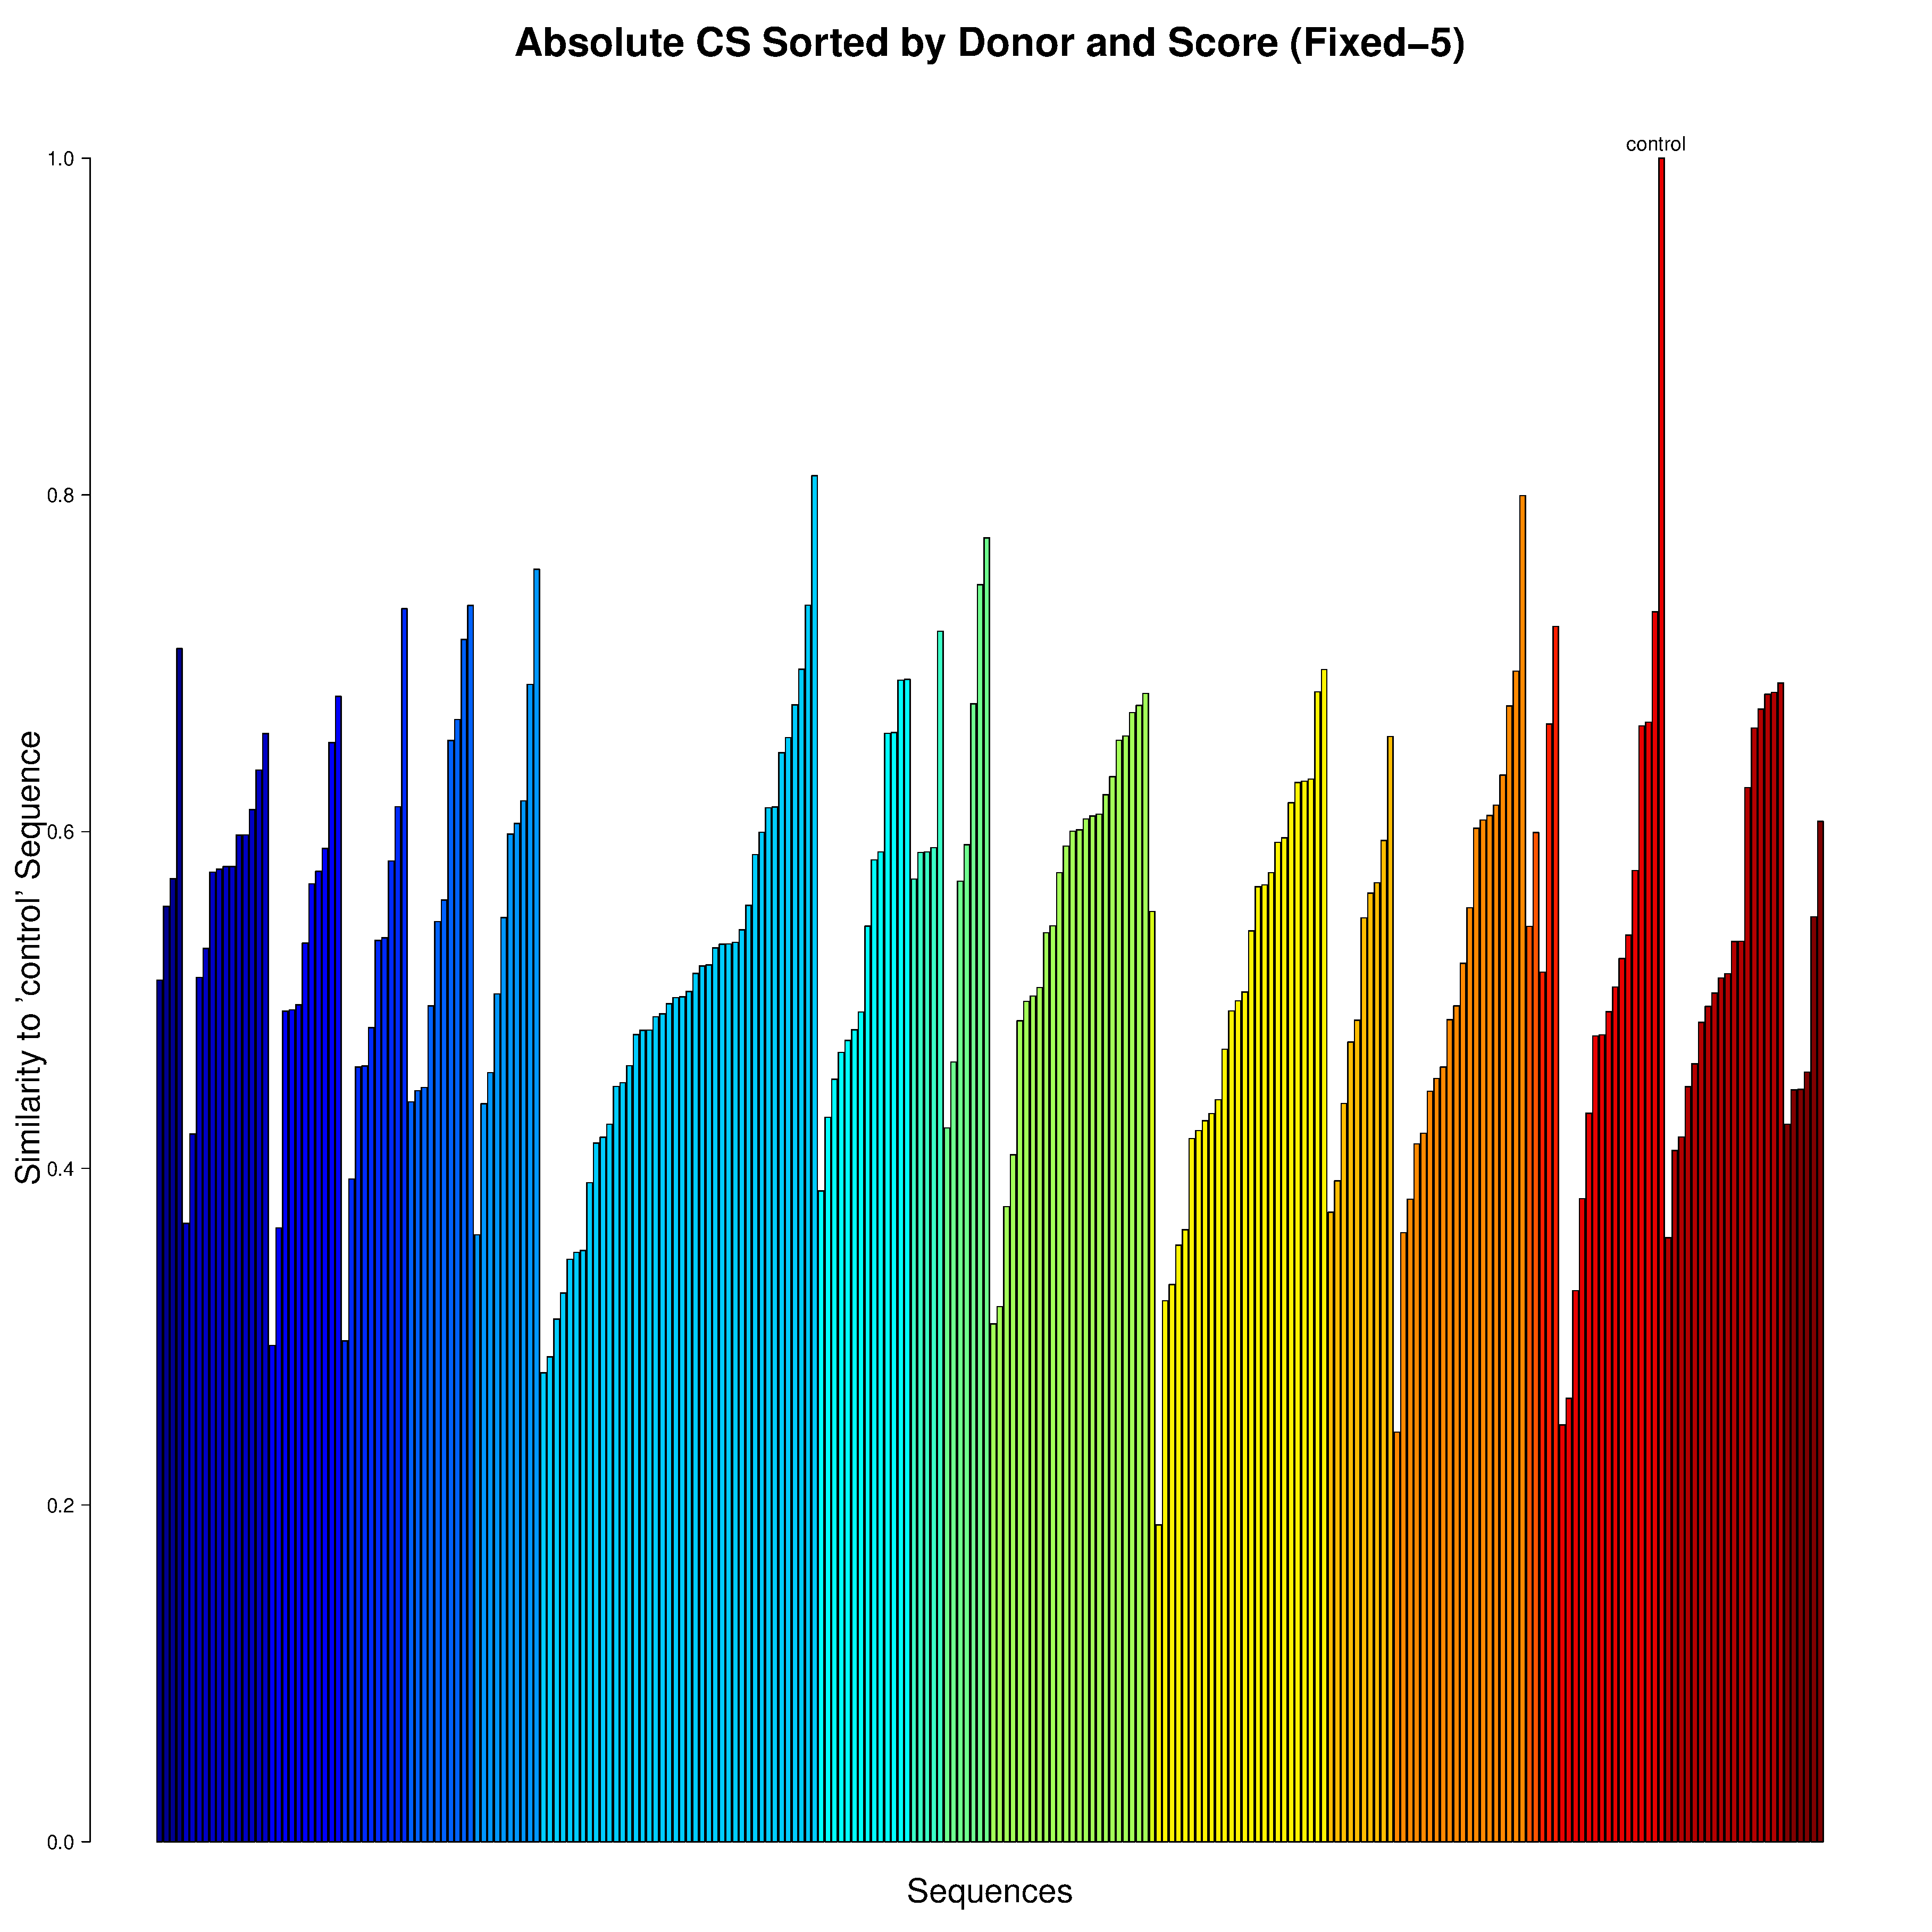
\includegraphics[width=0.4\linewidth]{ordered_by_Donor-Score_PC_Fixed-5}
	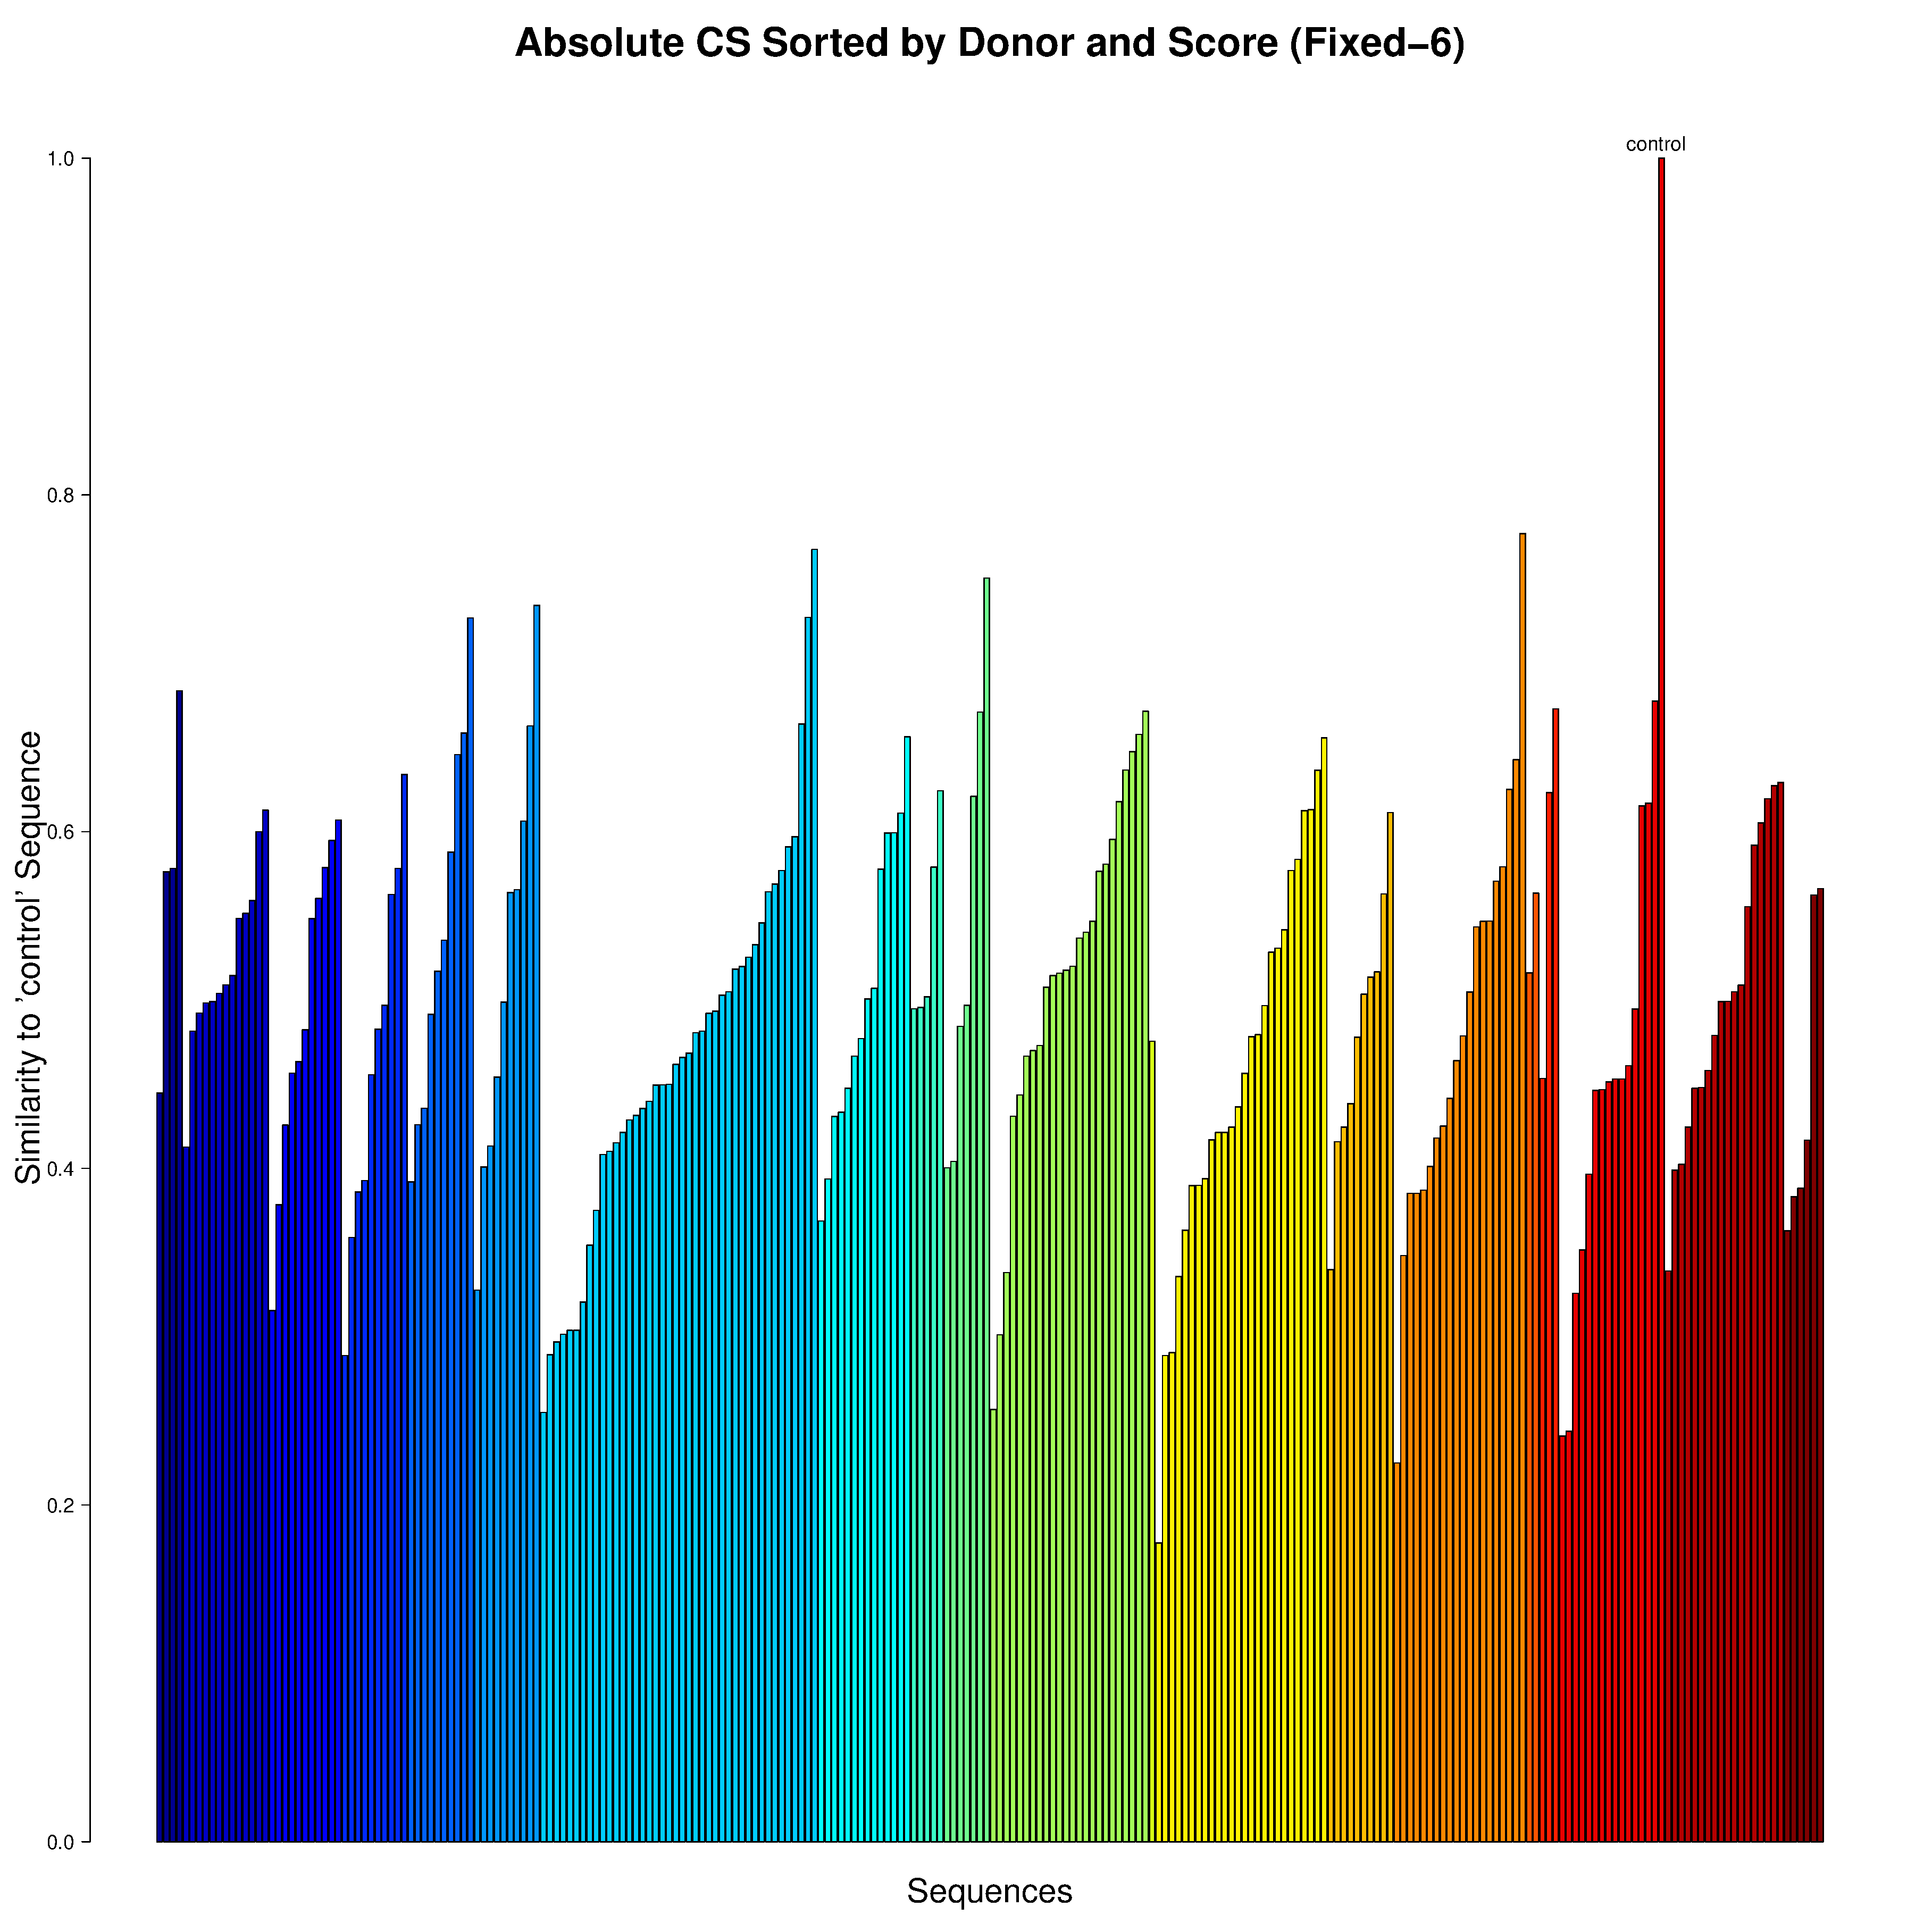
\includegraphics[width=0.4\linewidth]{ordered_by_Donor-Score_PC_Fixed-6}
\end{figure*}
\begin{figure*}
	\centering
	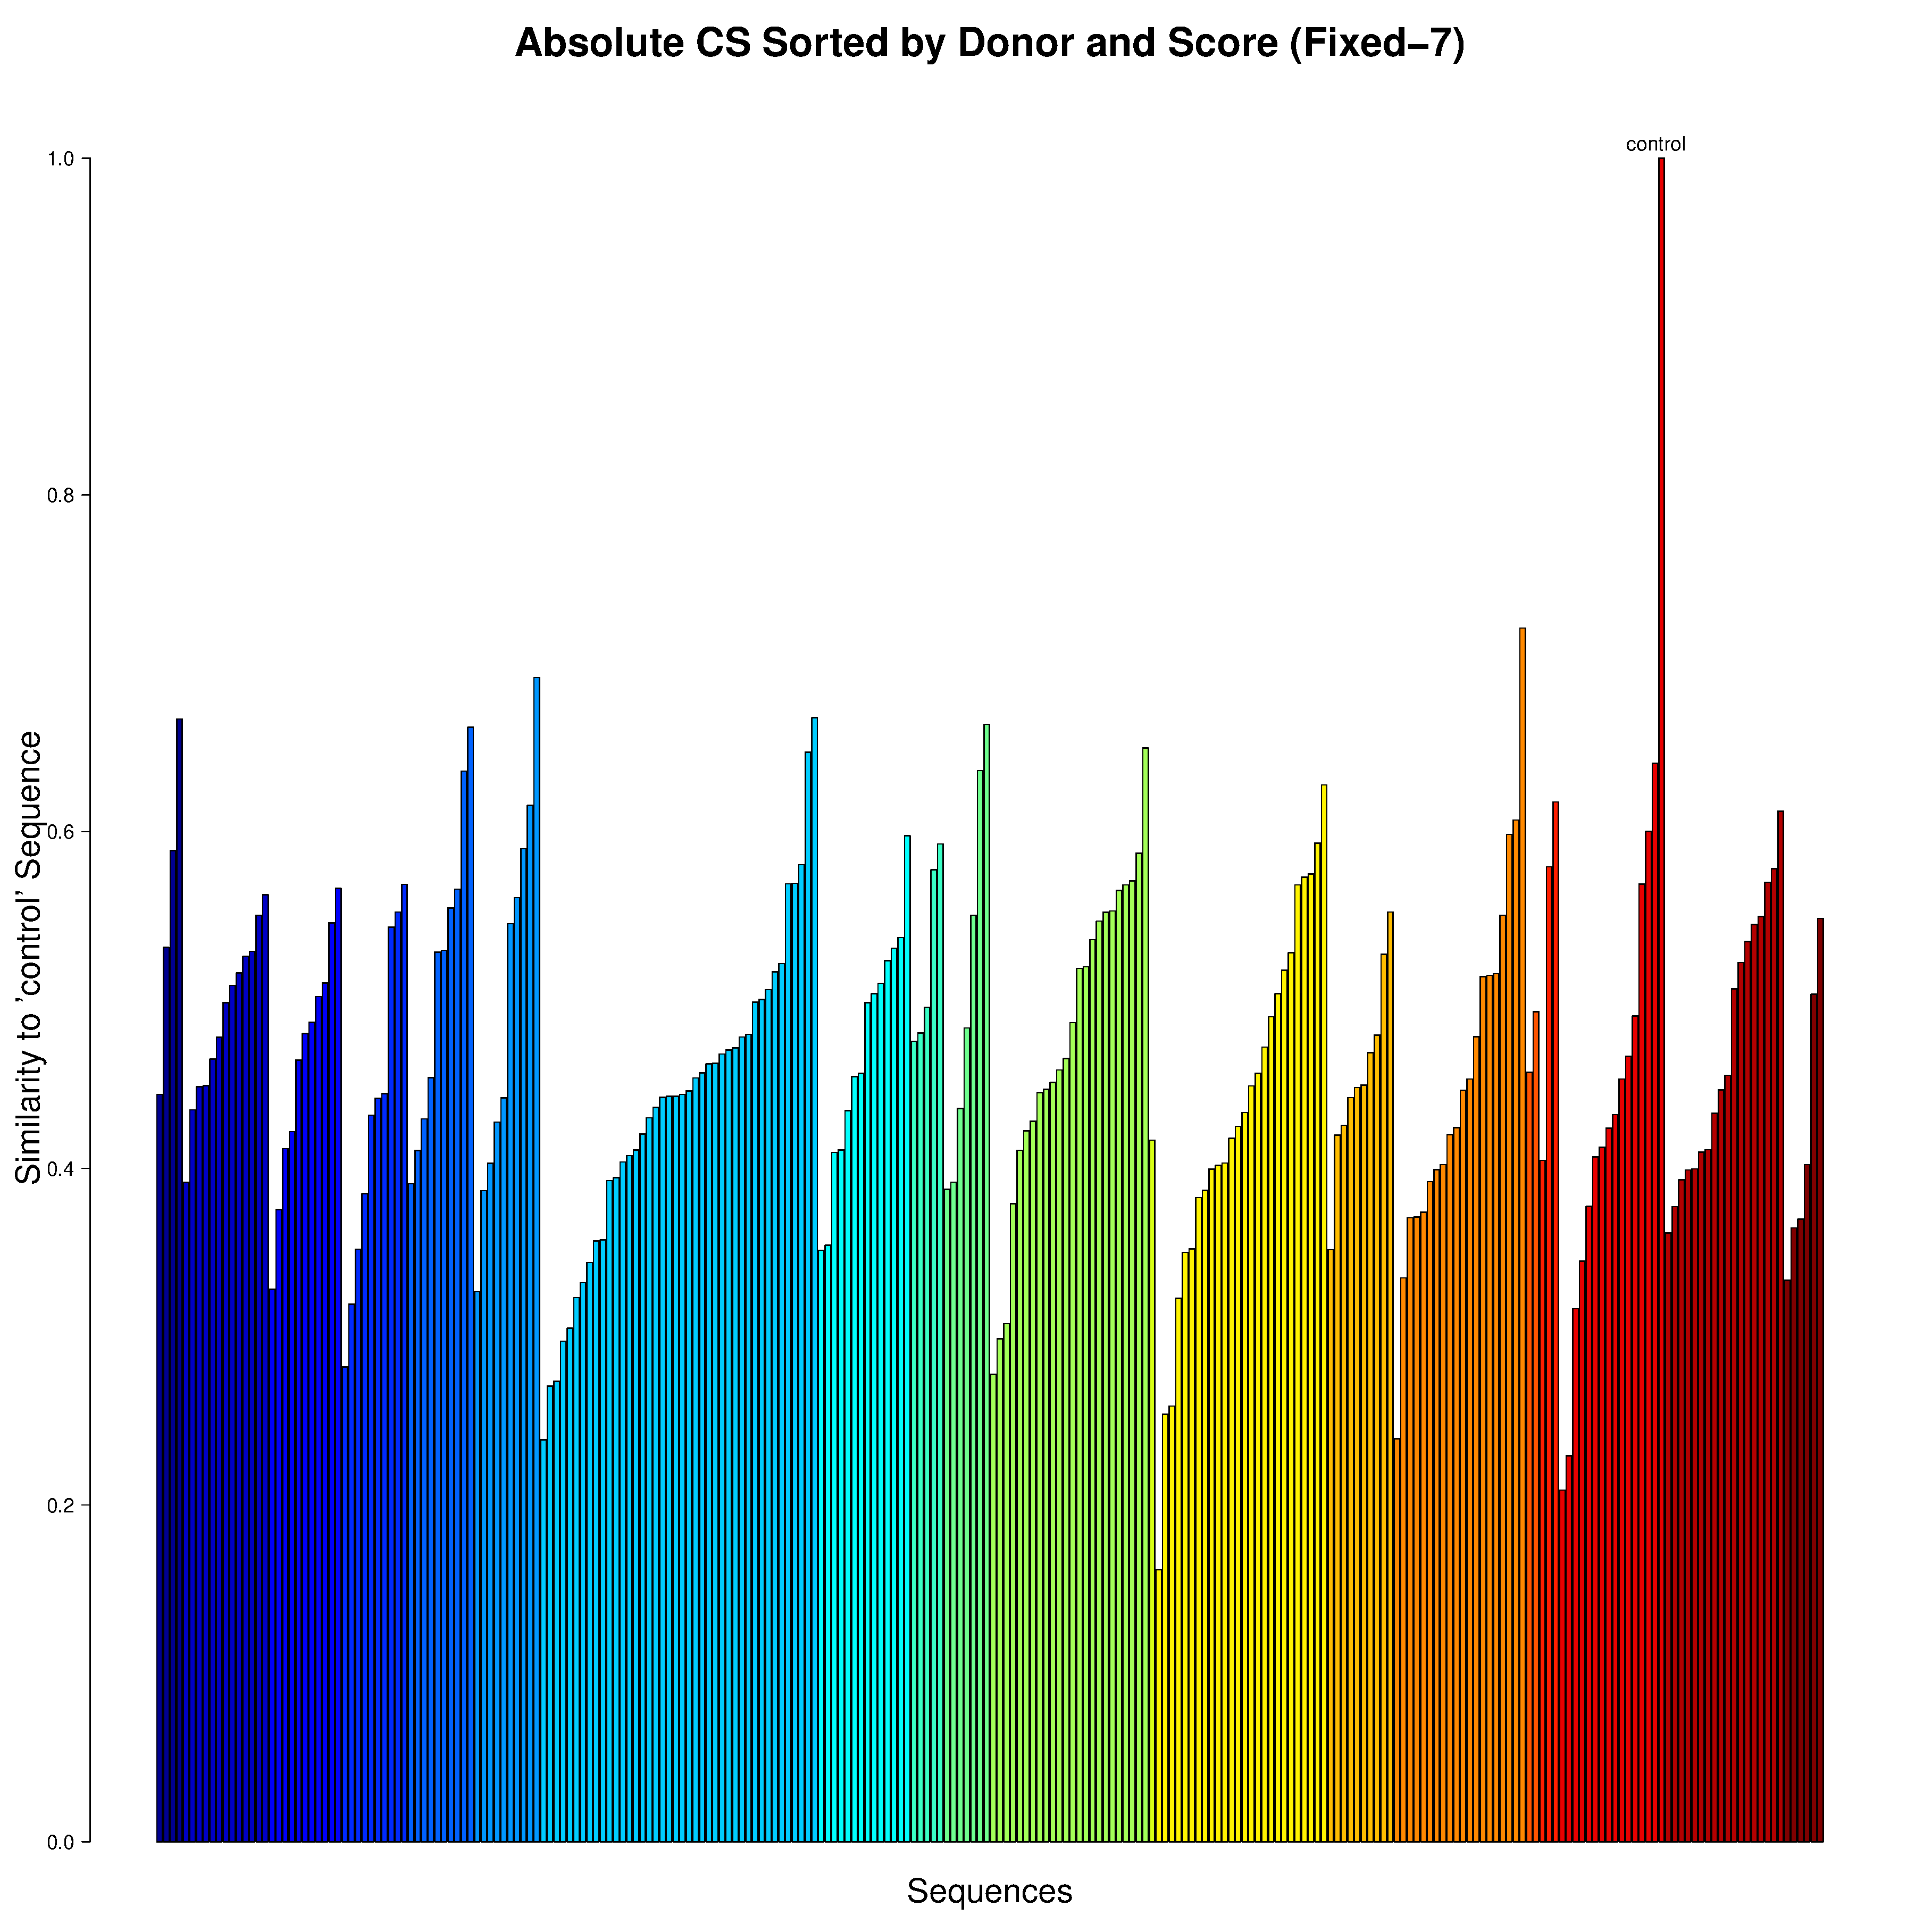
\includegraphics[width=0.4\linewidth]{ordered_by_Donor-Score_PC_Fixed-7}
	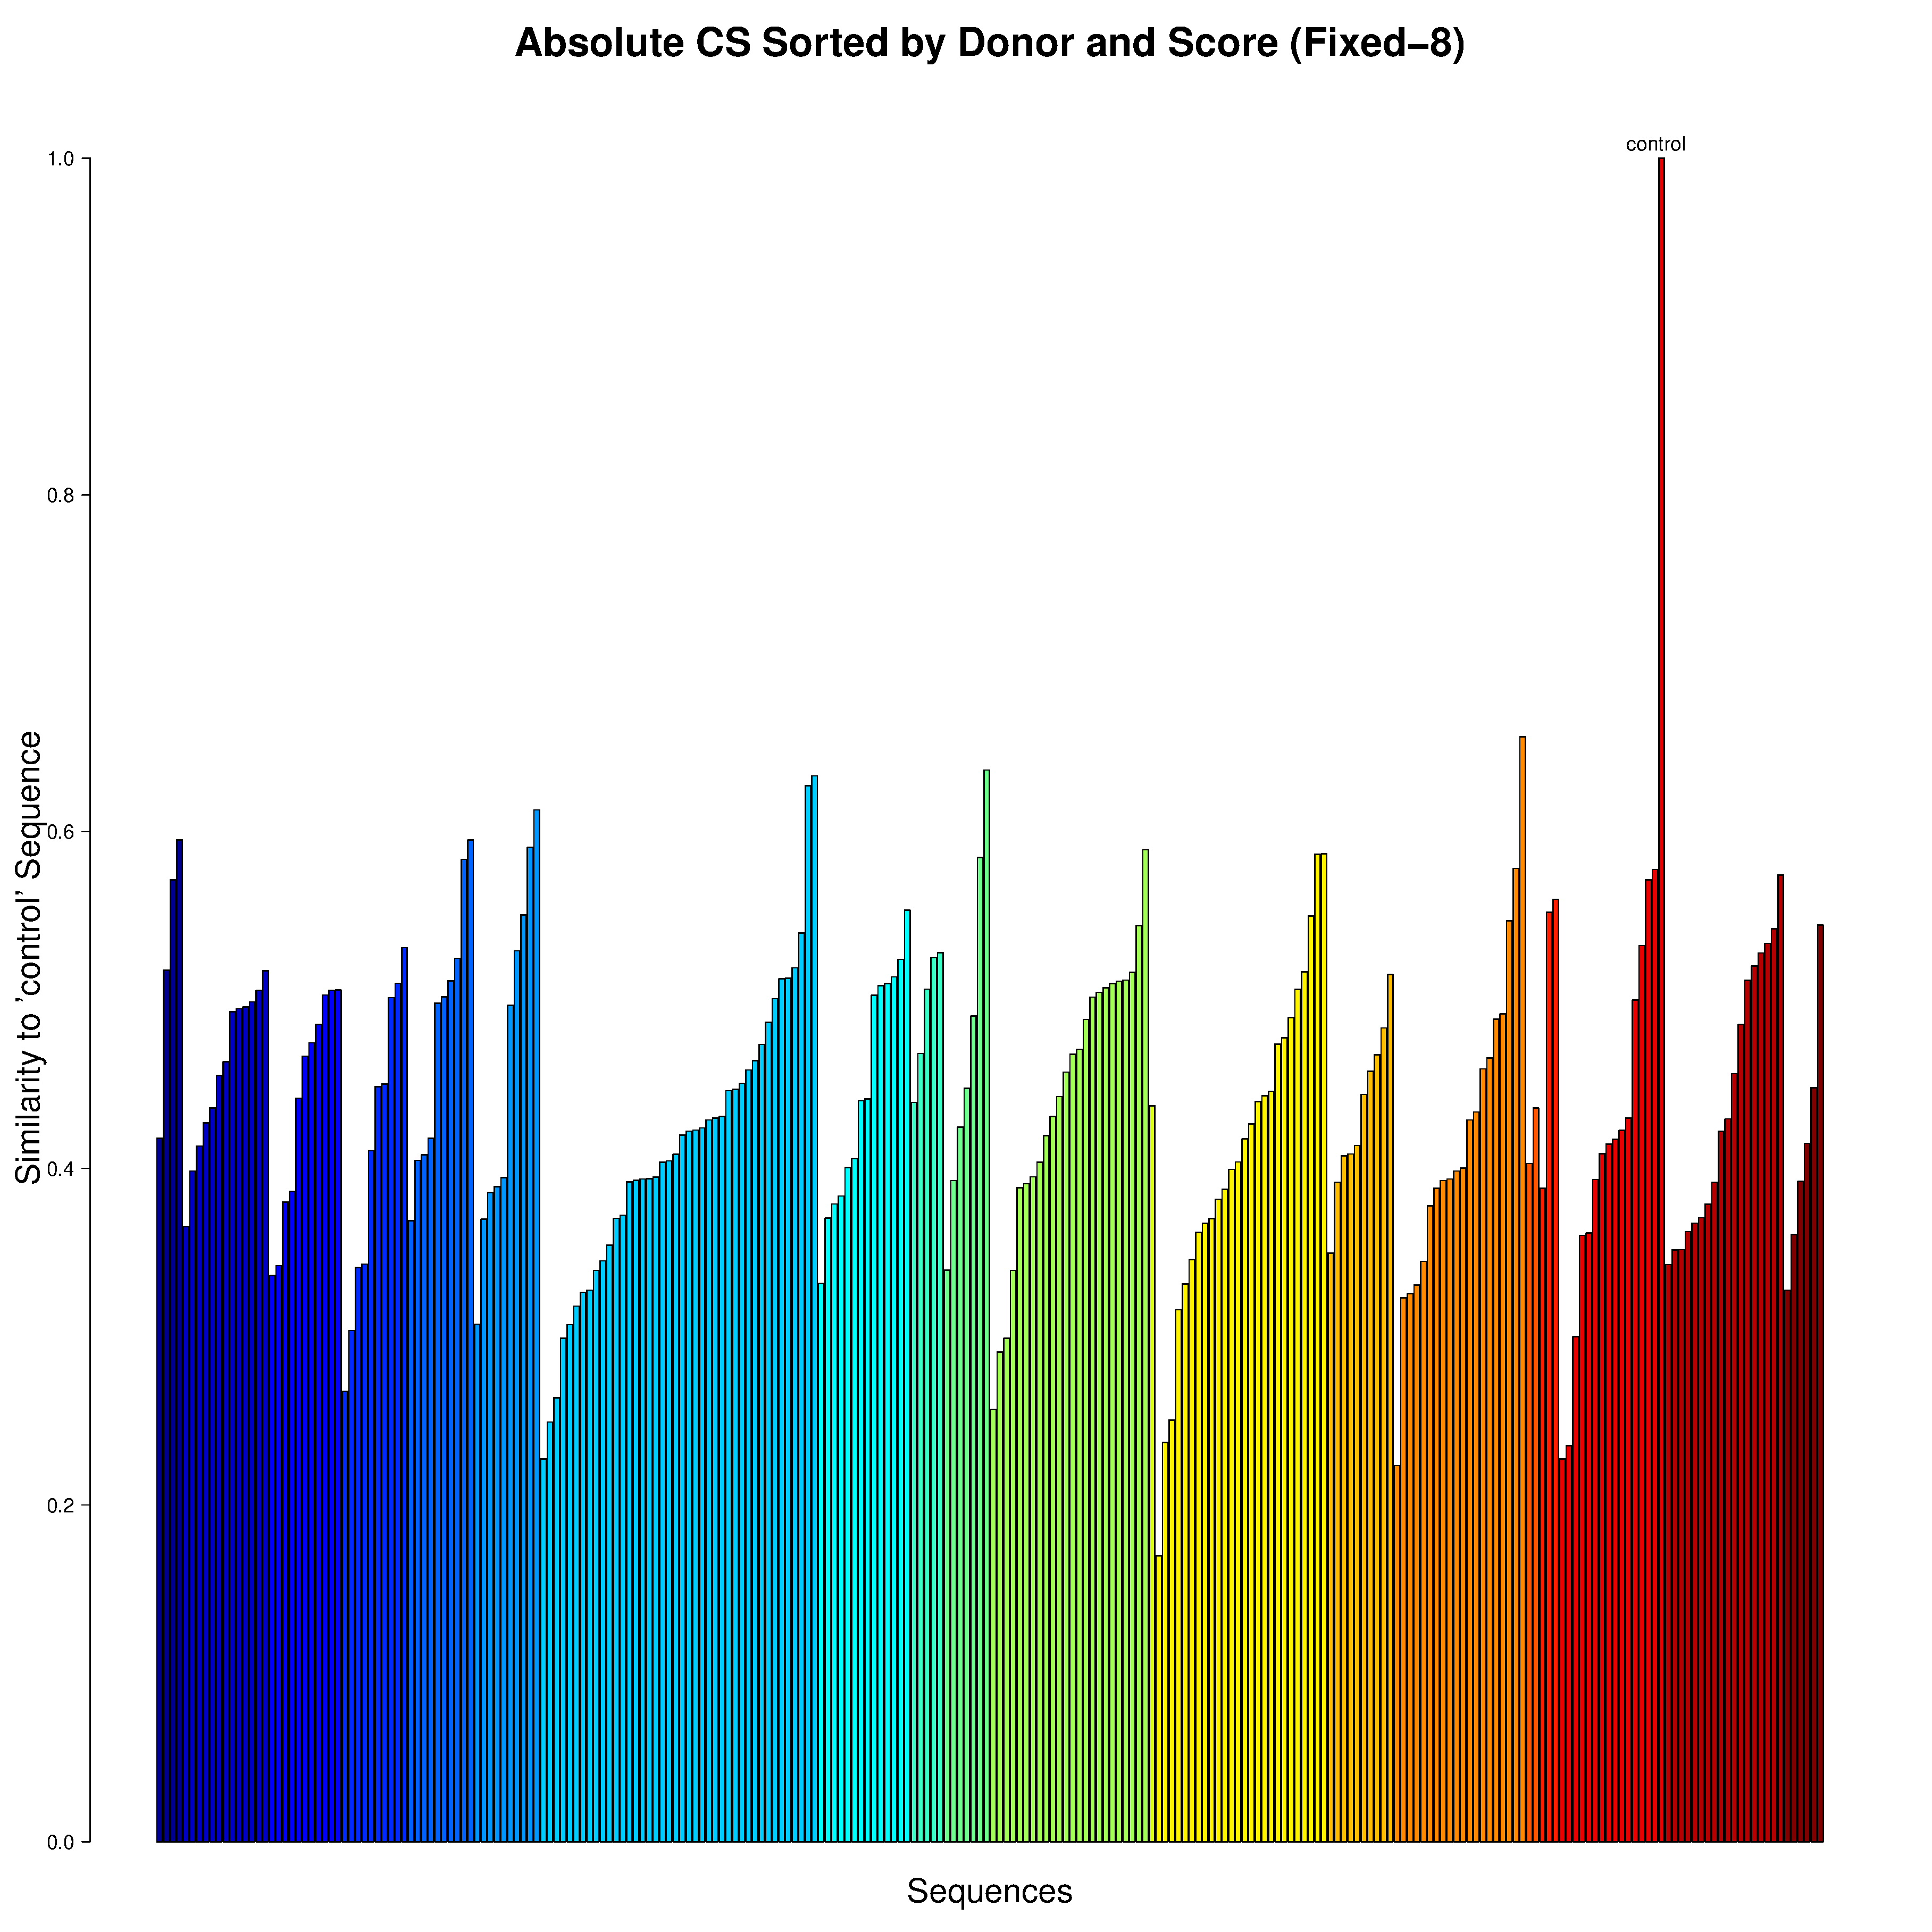
\includegraphics[width=0.4\linewidth]{ordered_by_Donor-Score_PC_Fixed-8}
\end{figure*}
\begin{figure*}
	\centering
	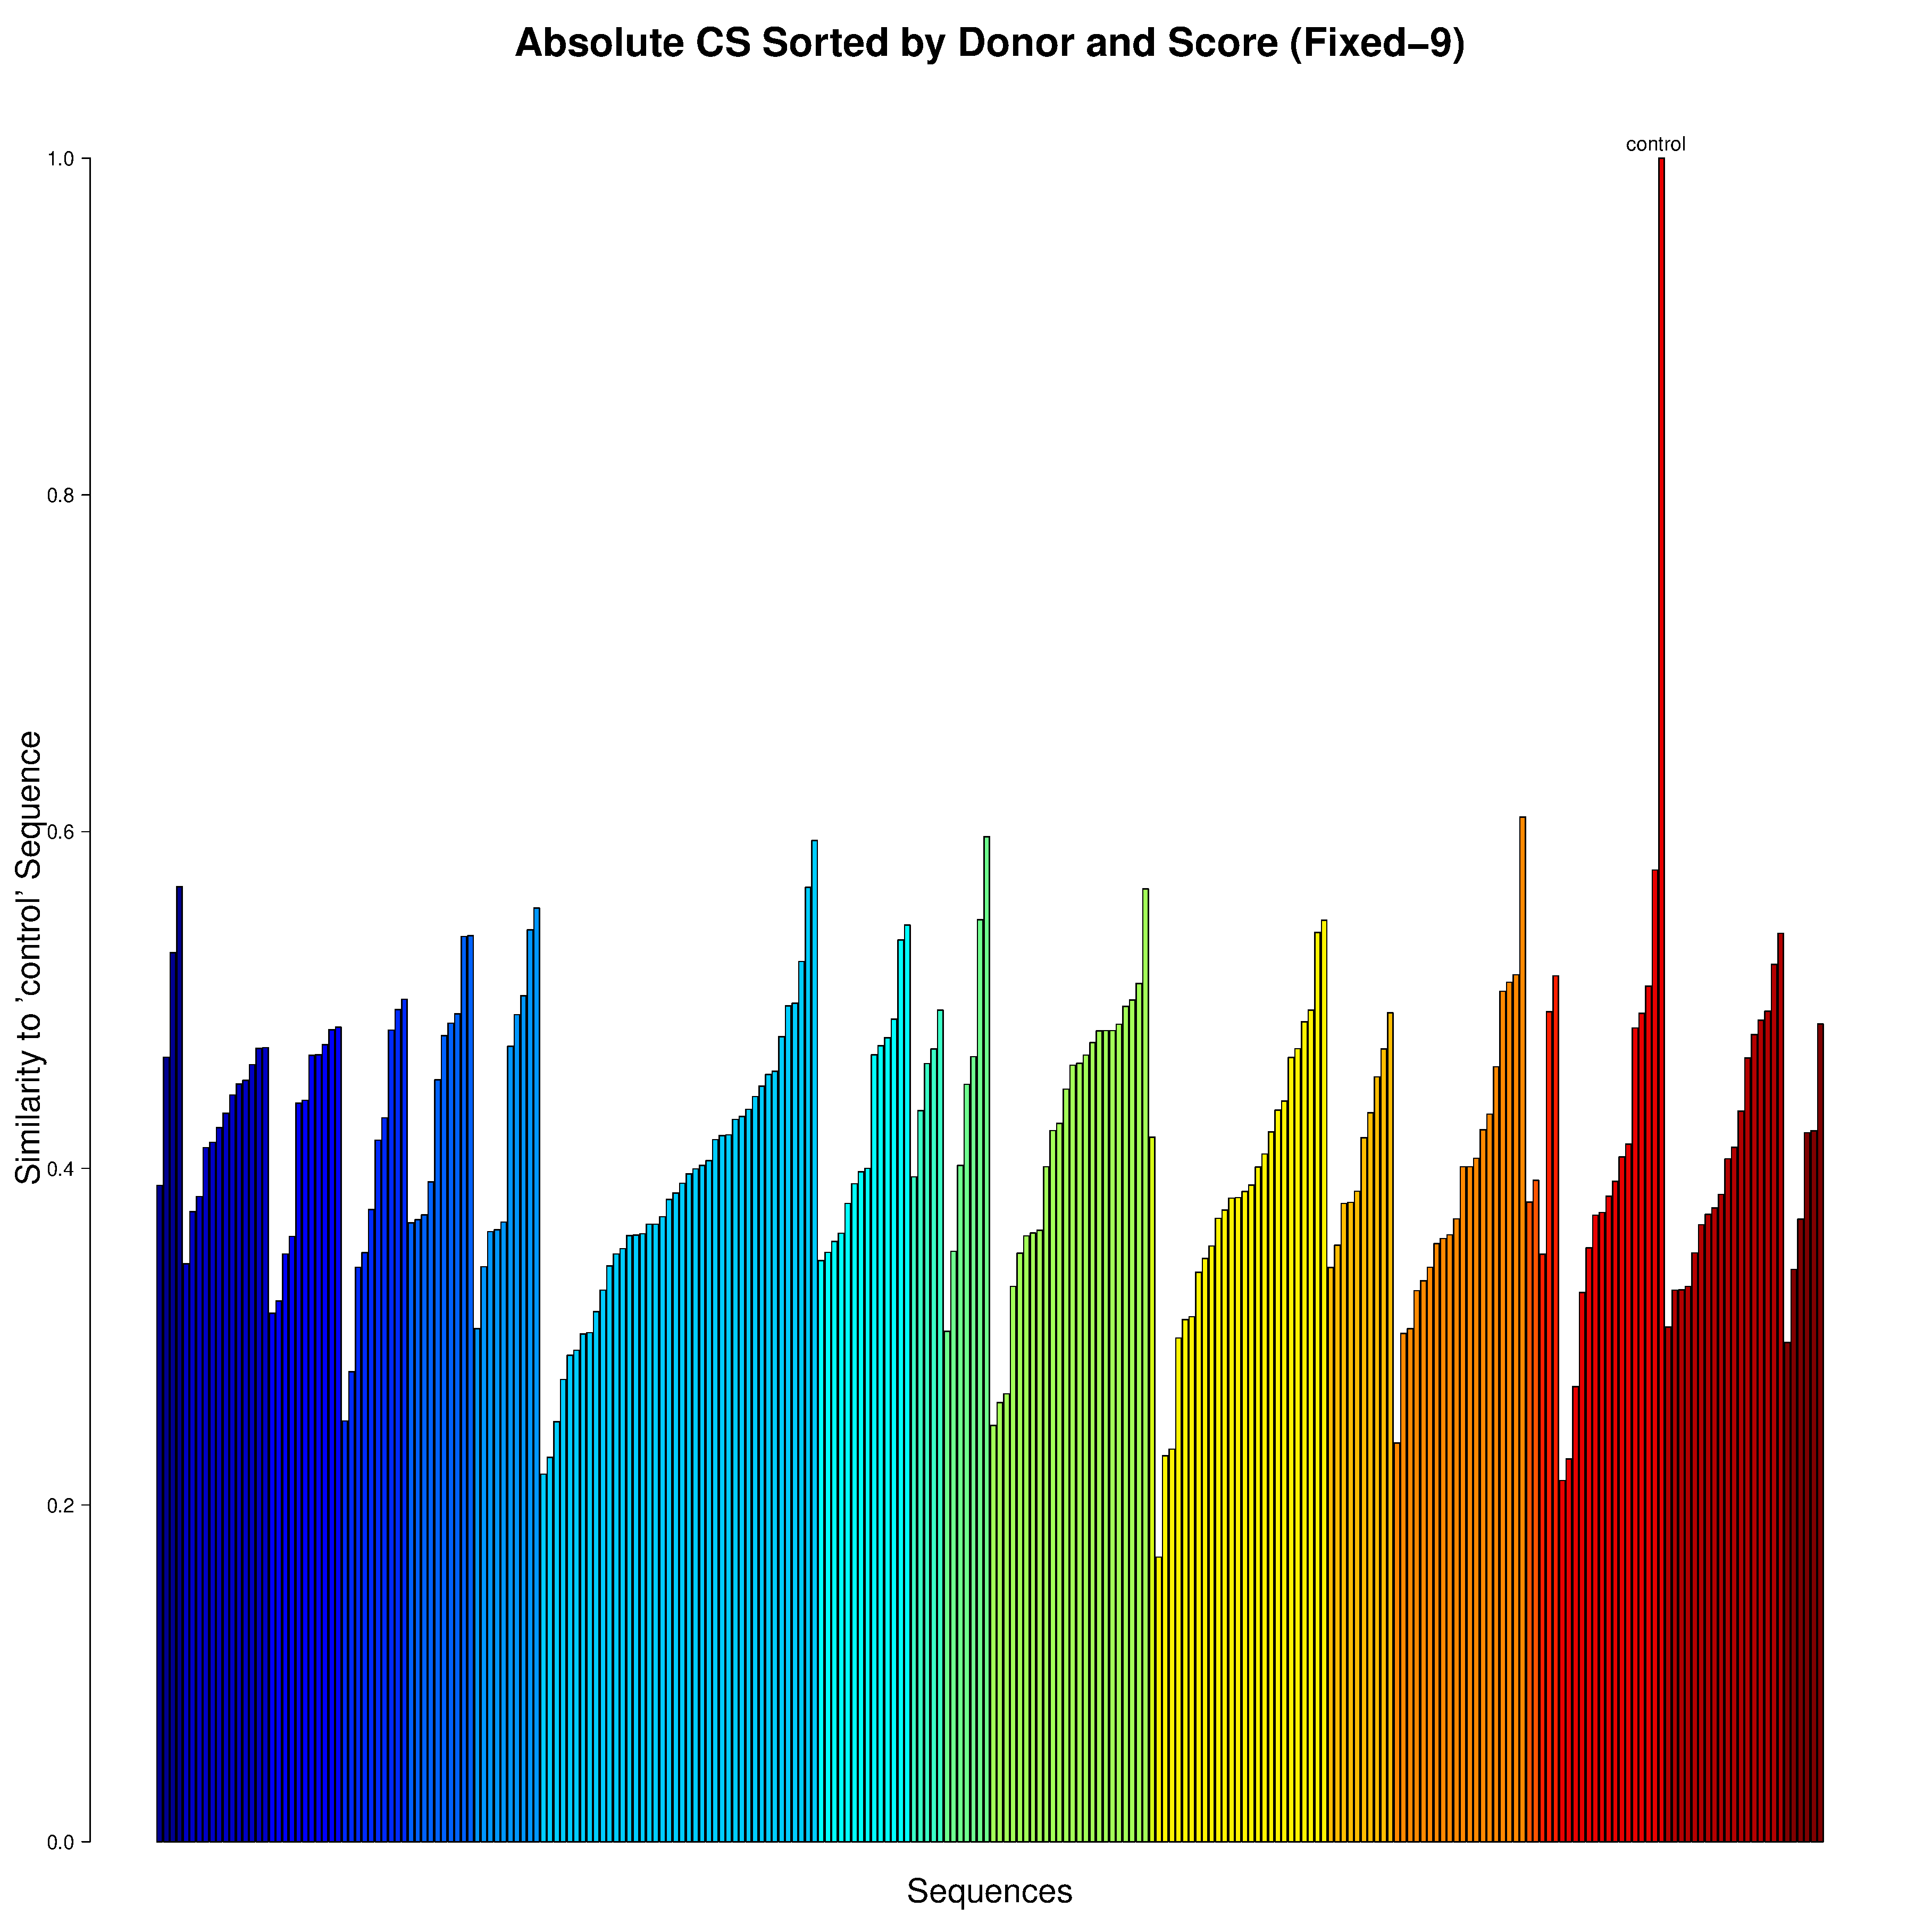
\includegraphics[width=0.4\linewidth]{ordered_by_Donor-Score_PC_Fixed-9}
	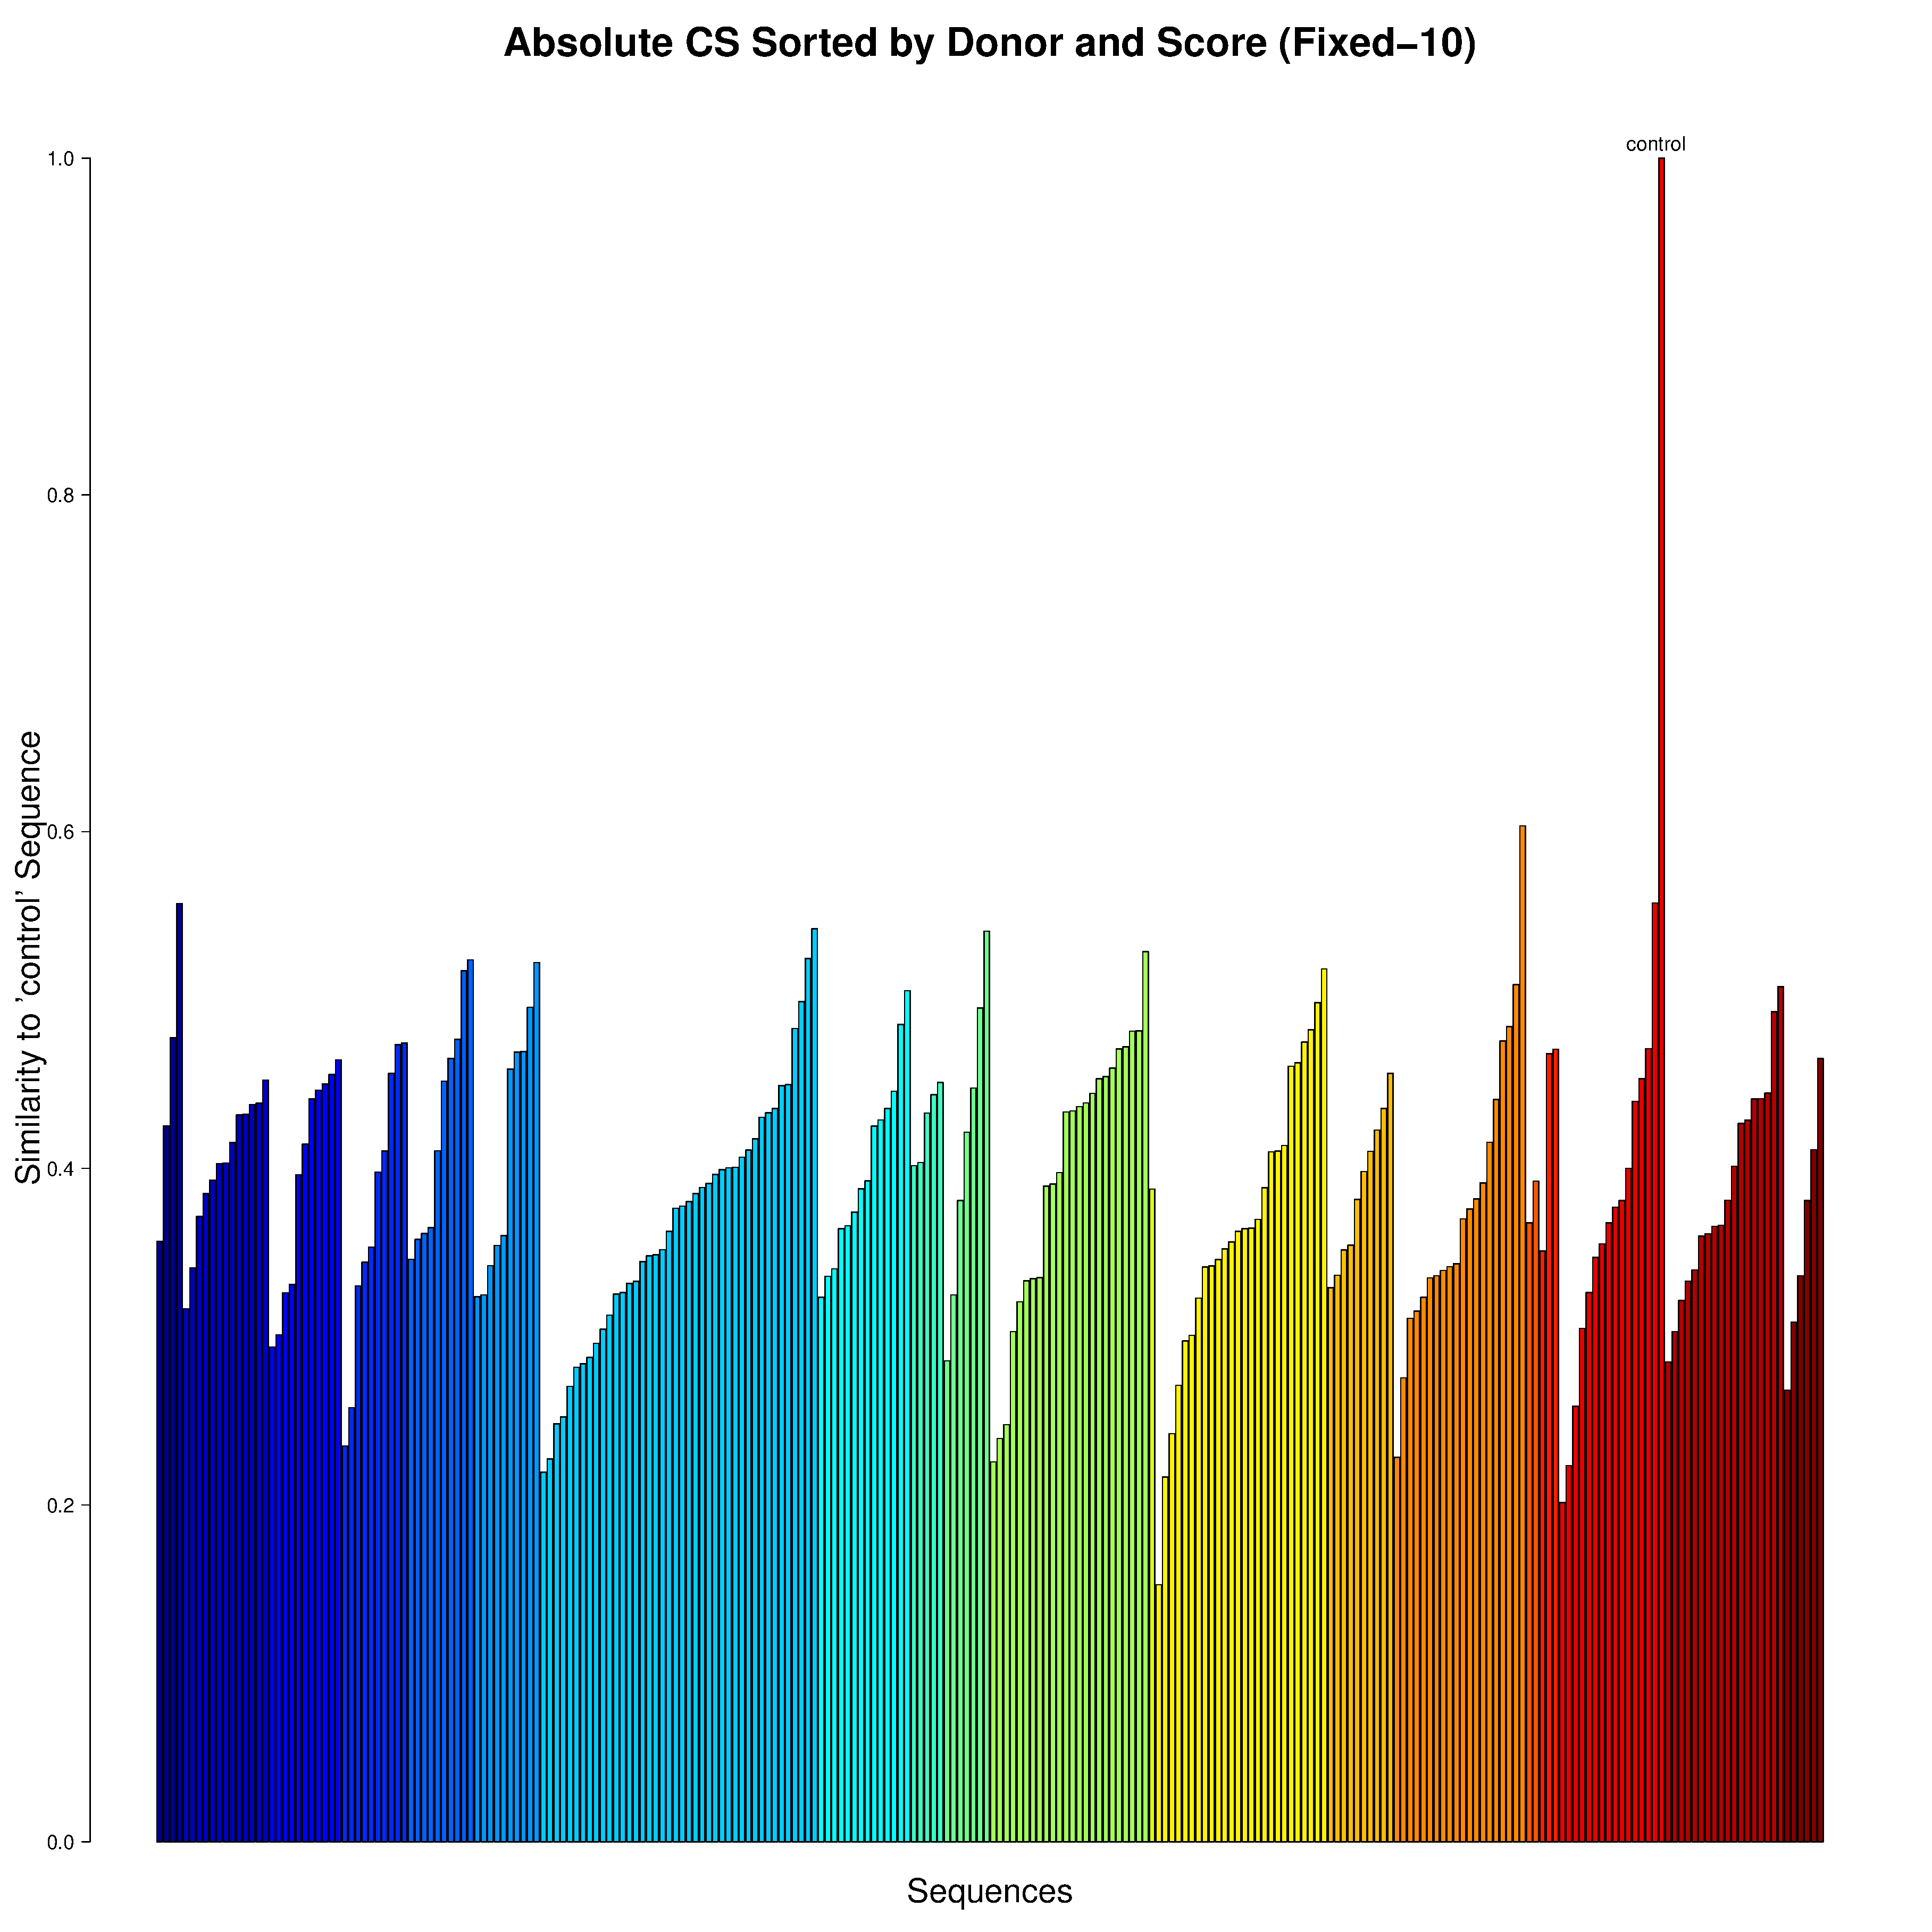
\includegraphics[width=0.4\linewidth]{ordered_by_Donor-Score_PC_Fixed-10}
\end{figure*}
% no \IEEEPARstart
%\hfill August 26, 2015
\newpage
\section{BESI vs. Phylogeny Trees}
We present here the entire set of phylogeny trees generated for this study along with the associated BESI scores side\textendash by\textendash side to simplify comparison and display the full potential of the BESI process to accurately classify structures based on a known or desired source.

\begin{table*}[]
	\begin{tabular}{ c c}
	\begin{minipage}{.4\textwidth}
	\raisebox{-\totalheight}{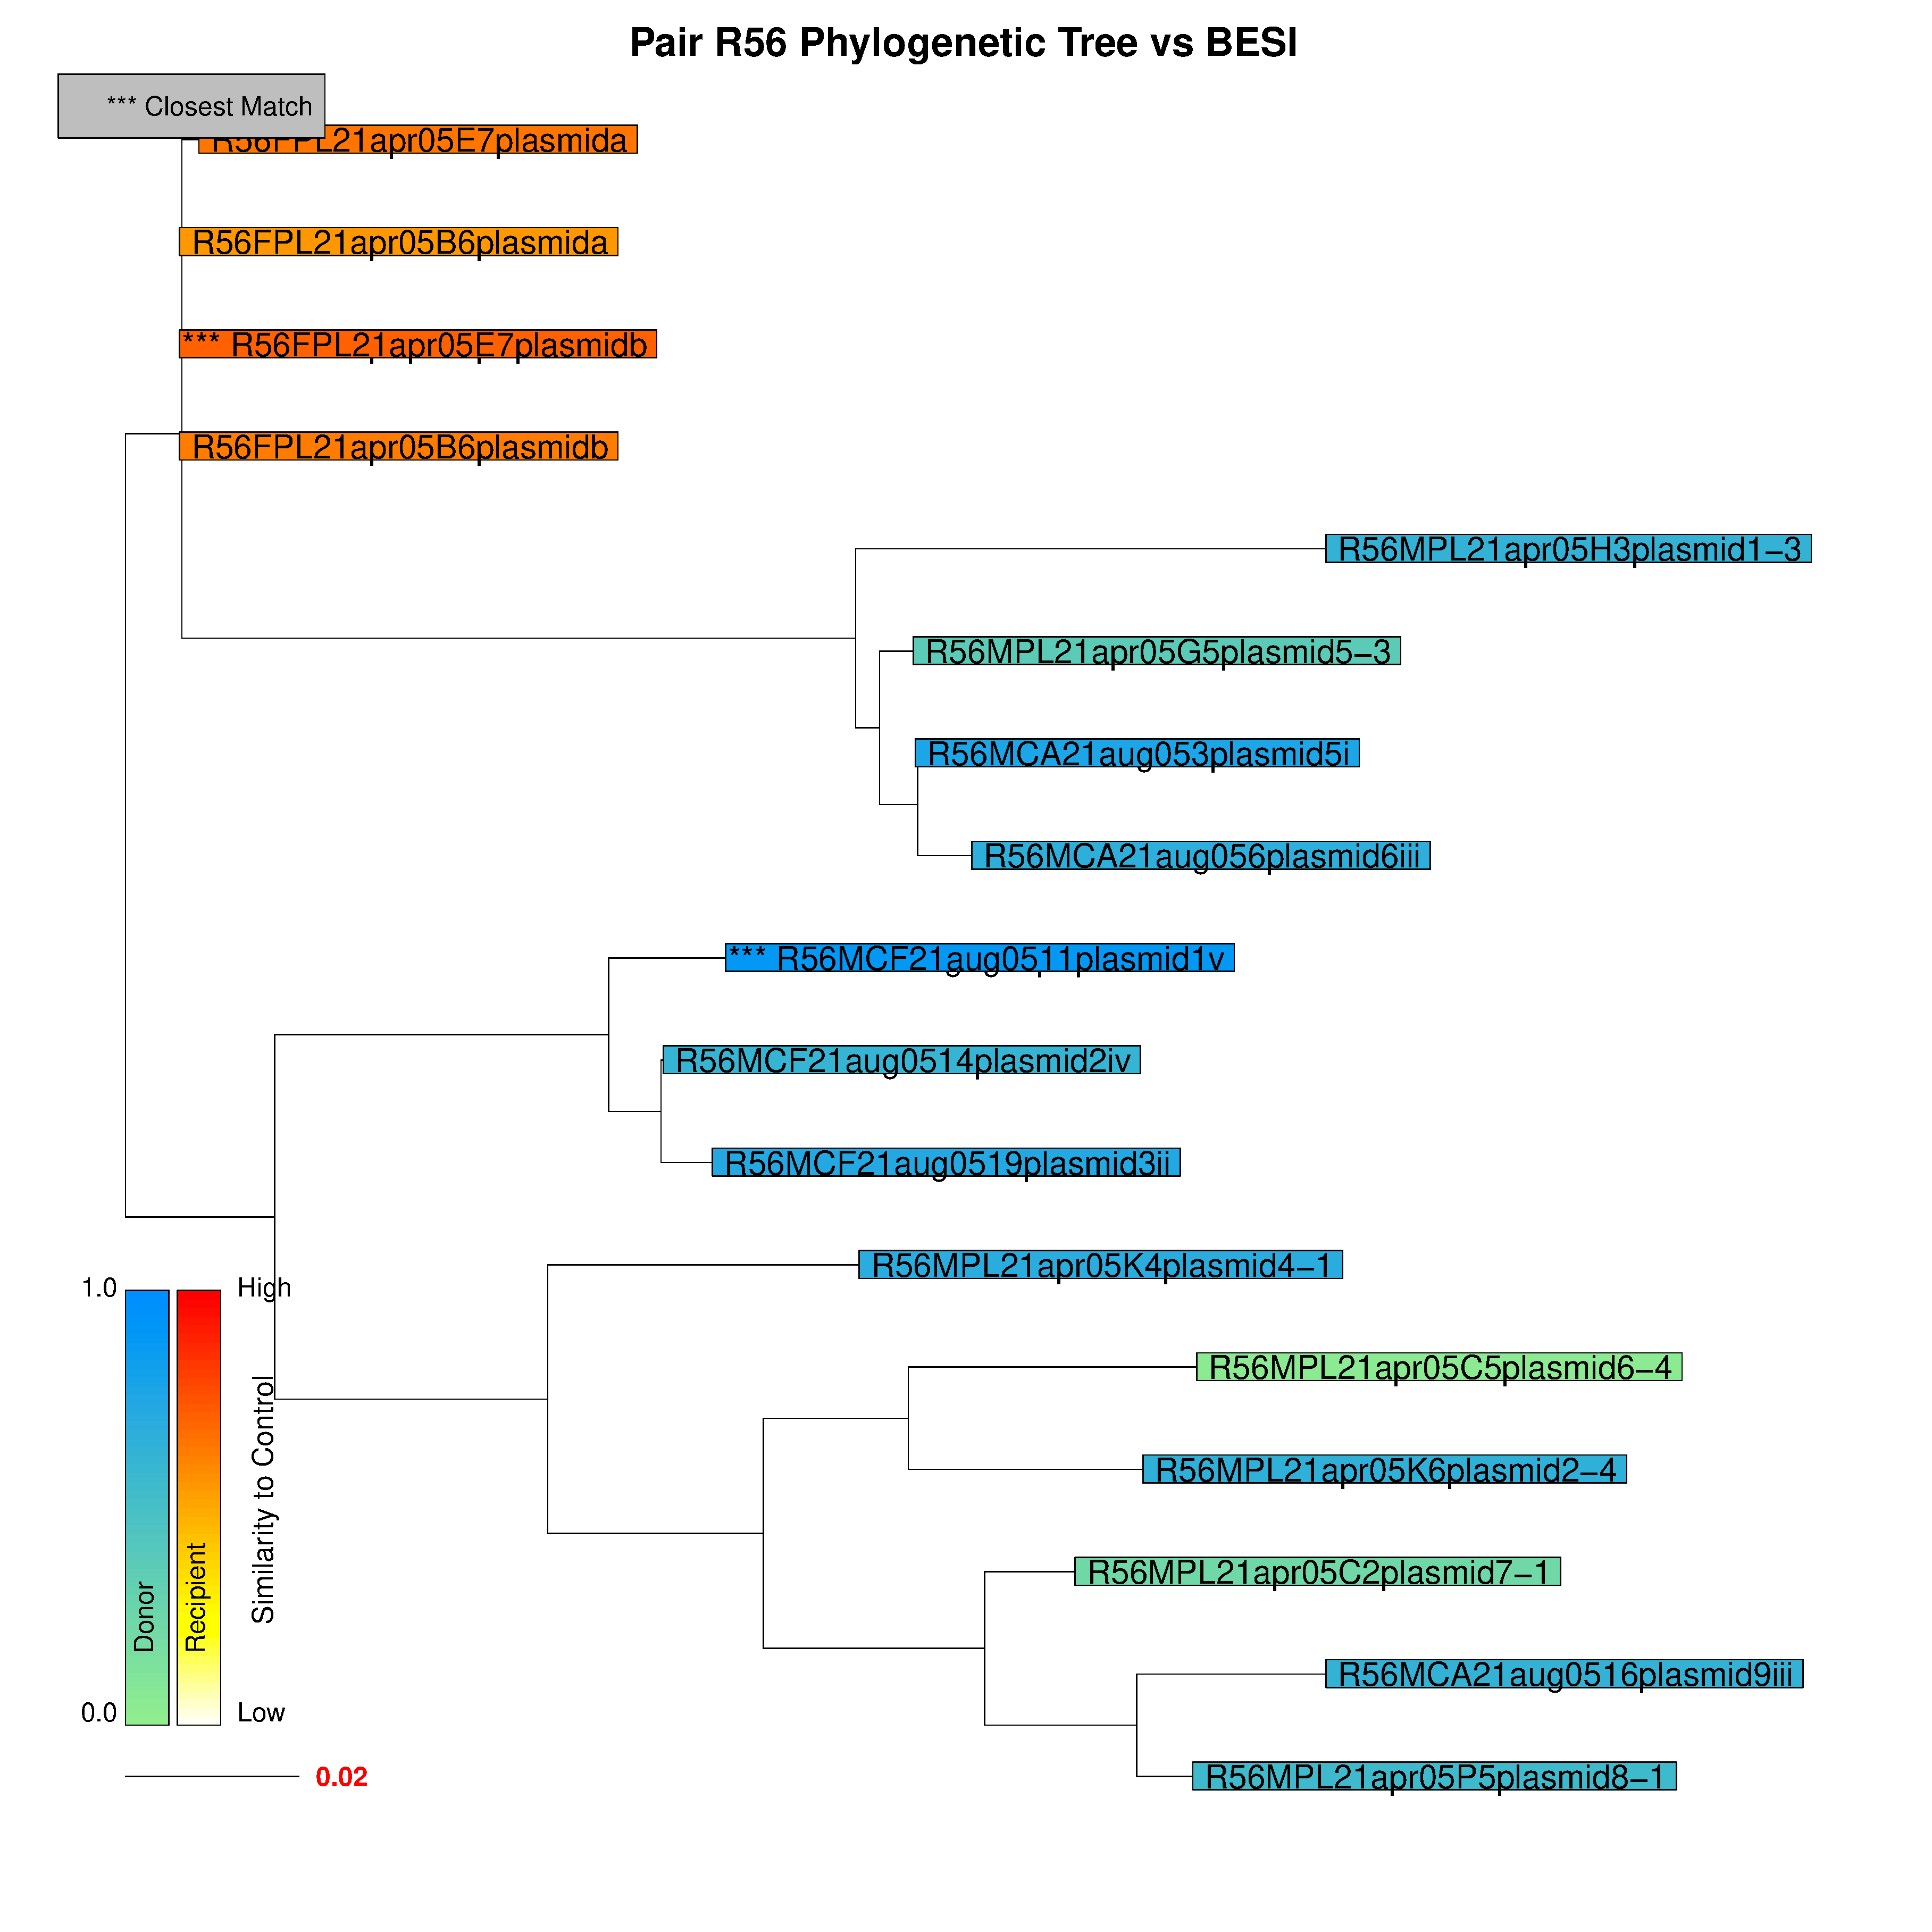
\includegraphics[width=\linewidth]{R56_heat_map_Fixed-2}} 
	\end{minipage}
	&	\begin{tabular}{l l l}
		\textbf{Role} & \textbf{Sequence} & \textbf{Score}\\
			\hline
			Recipient &R56FPL21apr05B6\_plasmid\_a	&	0.563919054126656	\\
						&R56FPL21apr05B6\_plasmid\_b	&	0.64914025990008	\\
						&R56FPL21apr05E7\_plasmid\_a	&	0.668113200596071	\\
						&R56FPL21apr05E7\_plasmid\_b	&	0.726523796985736	\\
			& \ &\ \\
			\hline
			Donor & R56MPL21apr05C5\_plasmid\_6-4	&	0.069038035927937	\\
						&R56MPL21apr05C2\_plasmid\_7-1	&	0.240246676350975	\\
						&R56MPL21apr05G5\_plasmid\_5-3	&	0.385319672126639	\\
						&R56MPL21apr05P5\_plasmid\_8-1	&	0.562805416203866	\\
						&R56MCF21aug0514\_plasmid\_2iv	&	0.624100461824737	\\
						&R56MPL21apr05H3\_plasmid\_1-3	&	0.641810107144584	\\
						&R56MCA21aug0516\_plasmid\_9iii	&	0.6510877349576	\\
						&R56MPL21apr05K6\_plasmid\_2-4	&	0.661026070503639	\\
						&R56MCA21aug056\_plasmid\_6iii	&	0.687419348128837	\\
						&R56MPL21apr05K4\_plasmid\_4-1	&	0.709966645467017	\\
						&R56MCF21aug0519\_plasmid\_3ii	&	0.752070920633736	\\
						&R56MCA21aug053\_plasmid\_5i	&	0.784921204312612	\\
						&R56MCF21aug0511\_plasmid\_1v	&	0.914998937284965	\\
					\end{tabular}\\
\hline
& \ \\
	\begin{minipage}{.4\textwidth}
	\raisebox{-\totalheight}{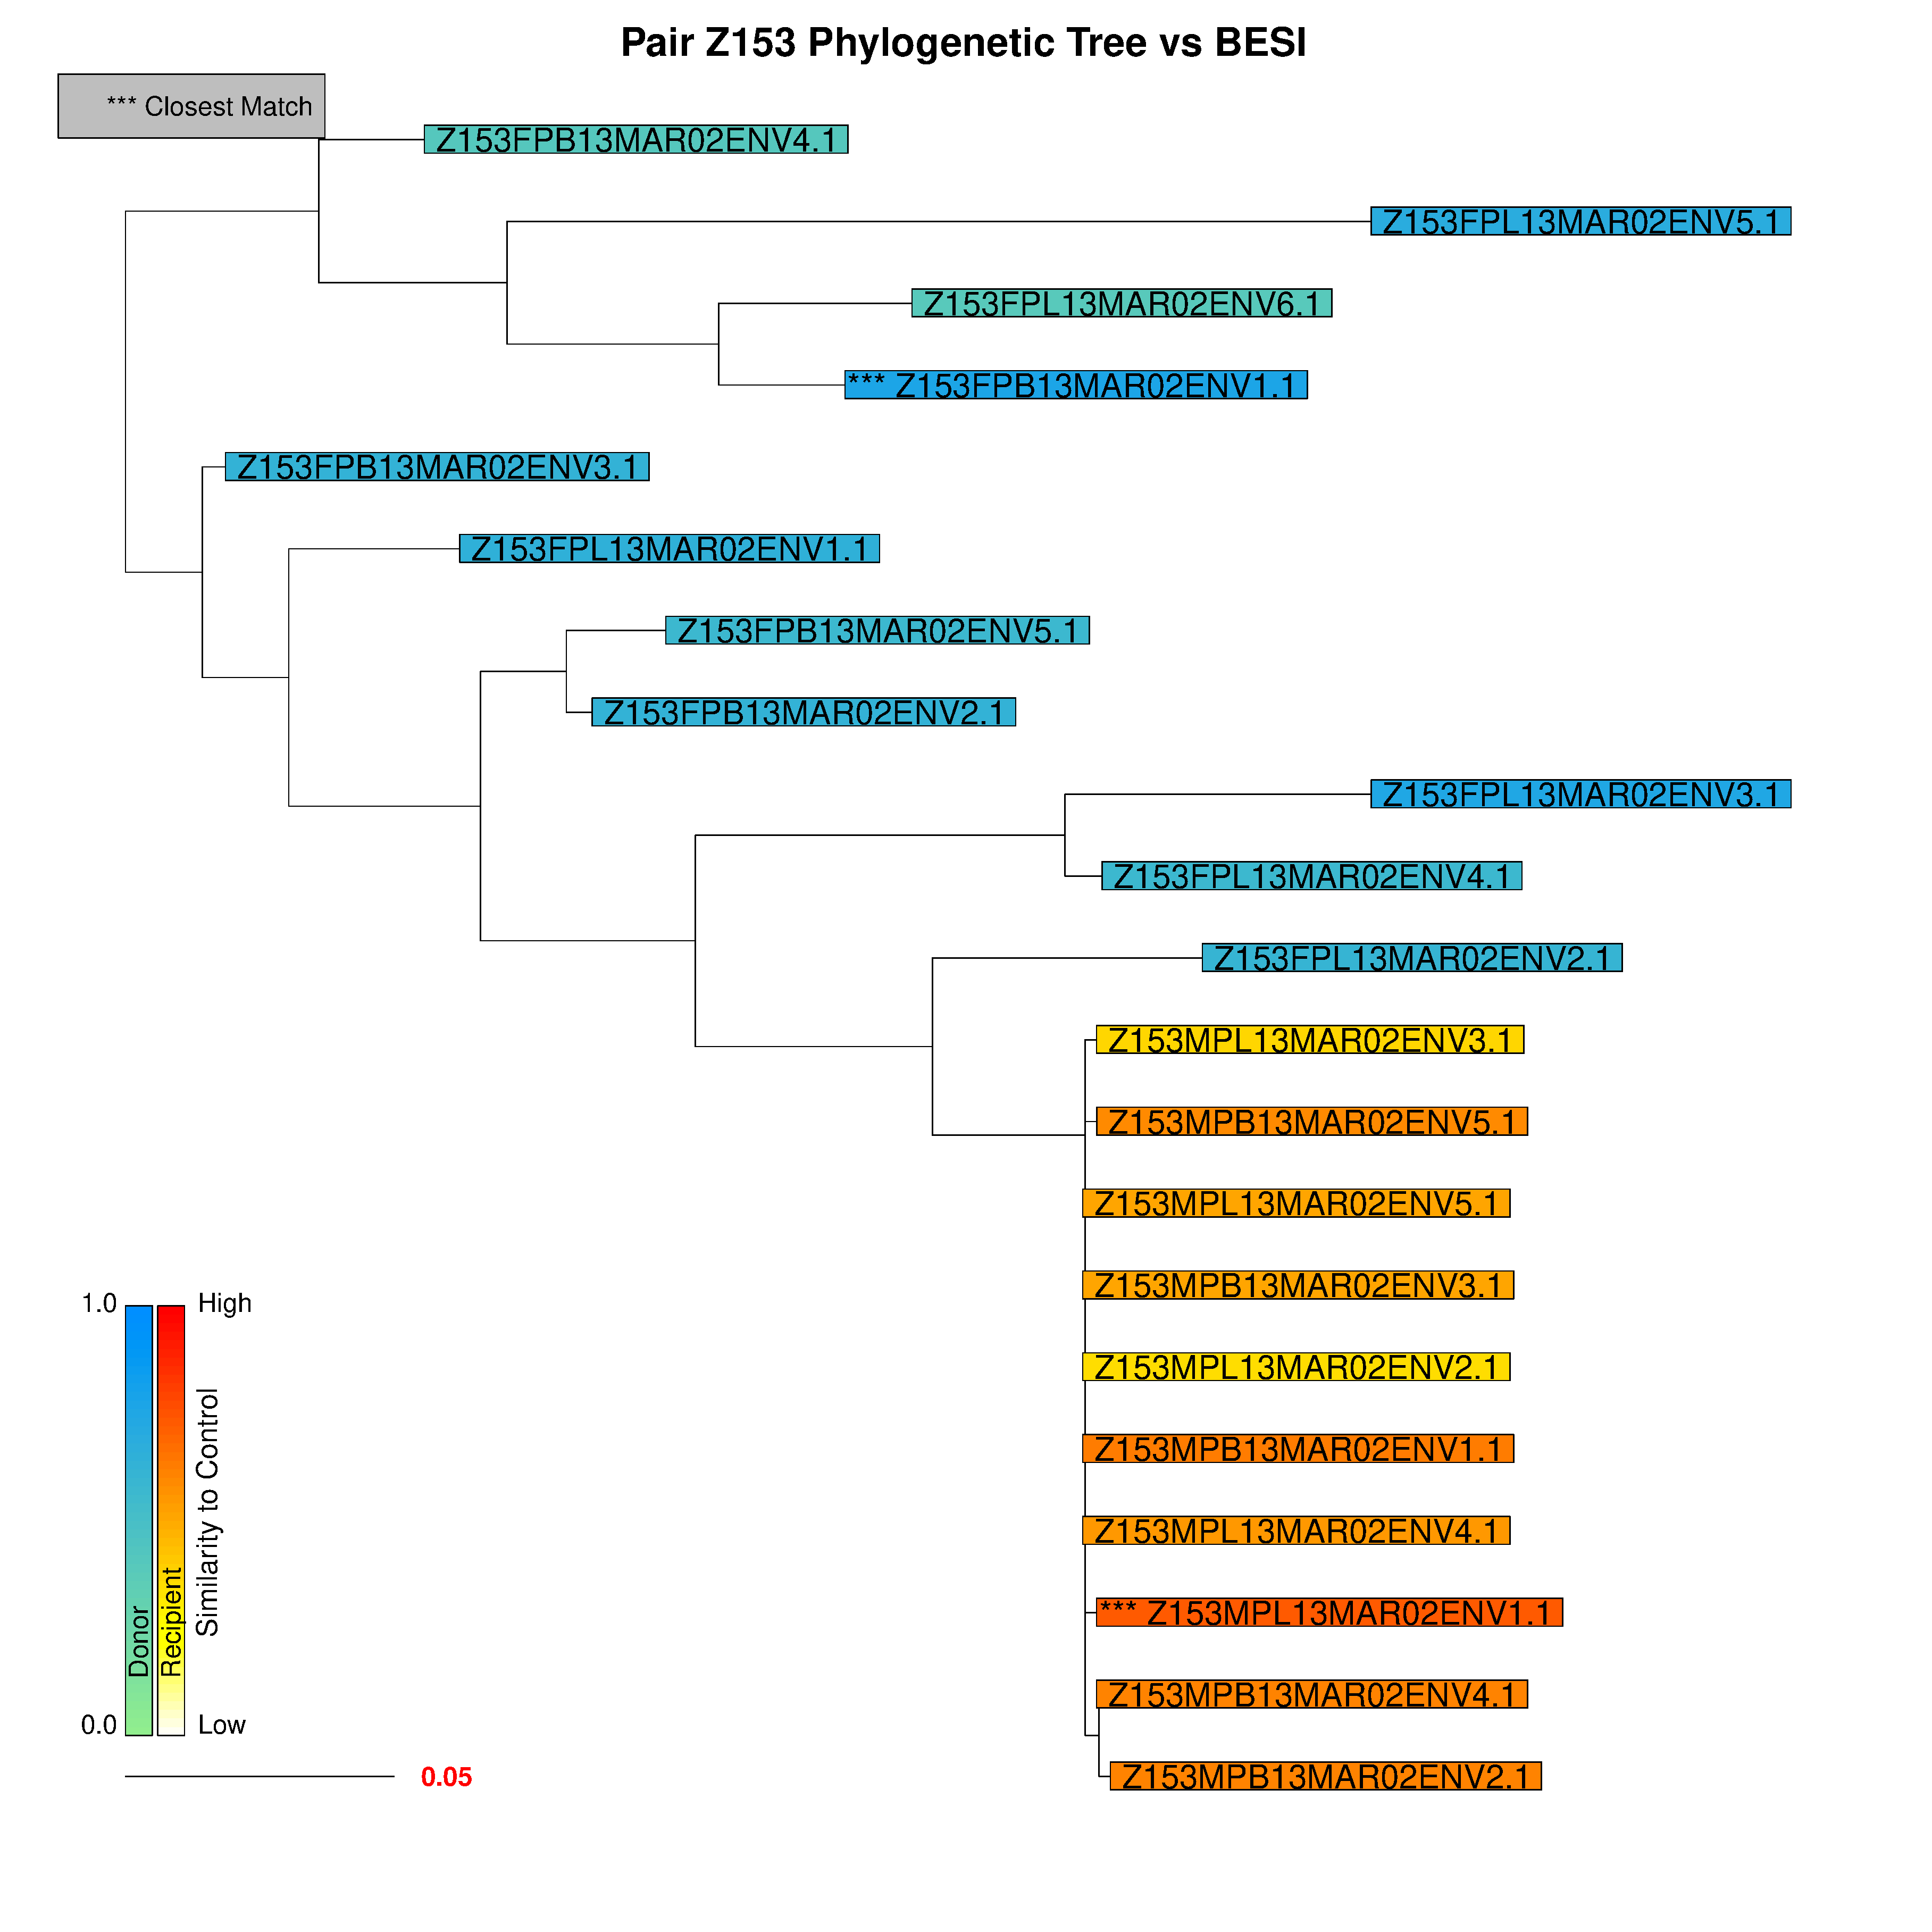
\includegraphics[width=\linewidth]{Z153_heat_map_Fixed-2}} 
\end{minipage}
&	\begin{tabular}{l l l}
		\textbf{Role} & \textbf{Sequence} & \textbf{Score}\\
	\hline
Donor &	Z153FPL13MAR02ENV6.1	&	0.400037903712386	\\
&	Z153FPB13MAR02ENV4.1	&	0.434302534517453	\\
&	Z153FPB13MAR02ENV5.1	&	0.592981403440573	\\
&	Z153FPL13MAR02ENV4.1	&	0.597555445982449	\\
&	Z153FPL13MAR02ENV2.1	&	0.623561198931831	\\
&	Z153FPB13MAR02ENV3.1	&	0.641829024257597	\\
&	Z153FPB13MAR02ENV2.1	&	0.65346062795849	\\
&	Z153FPL13MAR02ENV1.1	&	0.664666625866691	\\
&	Z153FPL13MAR02ENV5.1	&	0.705752387024319	\\
&	Z153FPL13MAR02ENV3.1	&	0.7729869980639	\\
&	Z153FPB13MAR02ENV1.1	&	0.780562081434307	\\
& \ &\ \\
\hline
Recipient &	Z153MPL13MAR02ENV2.1	&	0.378832825672163	\\
&	Z153MPL13MAR02ENV3.1	&	0.39739057280696	\\
&	Z153MPL13MAR02ENV5.1	&	0.531346002987244	\\
&	Z153MPB13MAR02ENV3.1	&	0.534273492833427	\\
&	Z153MPL13MAR02ENV4.1	&	0.576099624160442	\\
&	Z153MPB13MAR02ENV5.1	&	0.616979229776951	\\
&	Z153MPB13MAR02ENV4.1	&	0.636615493351413	\\
&	Z153MPB13MAR02ENV2.1	&	0.639562968980064	\\
&	Z153MPB13MAR02ENV1.1	&	0.653512495252073	\\
&	Z153MPL13MAR02ENV1.1	&	0.753213522009278	\\
\end{tabular}\\
\hline
& \ \\
\begin{minipage}{.4\textwidth}
	\raisebox{-\totalheight}{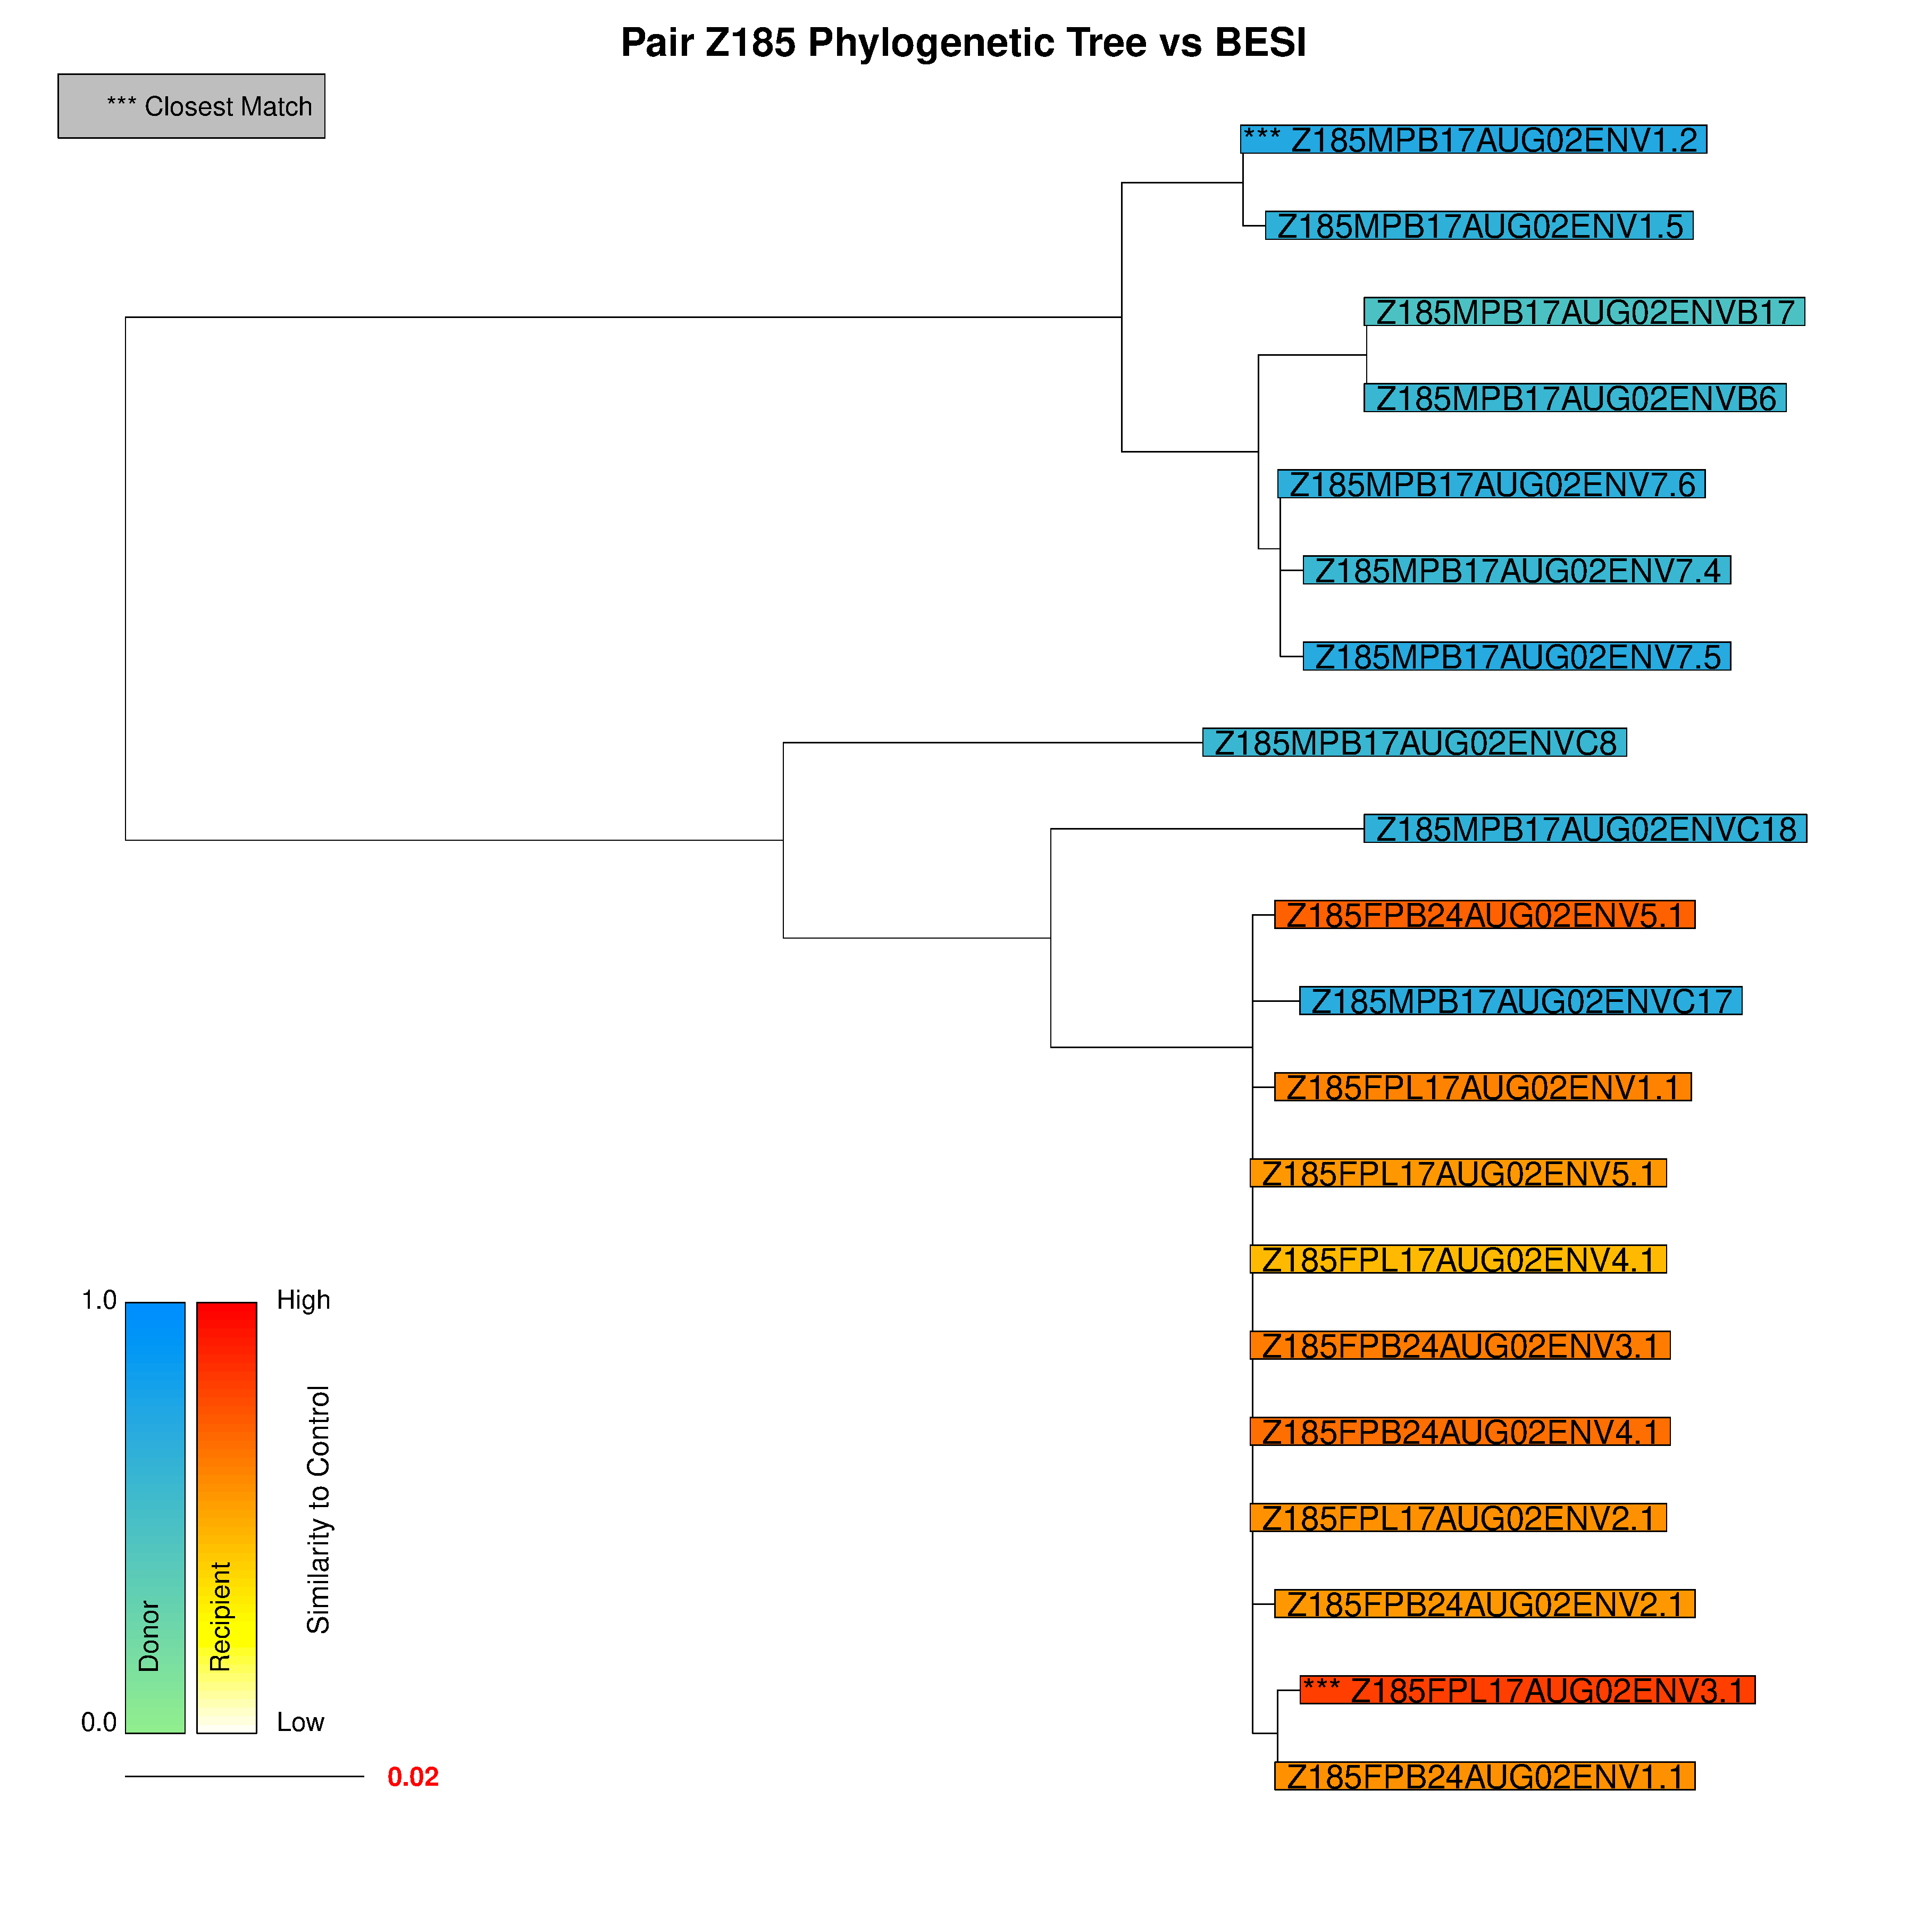
\includegraphics[width=\linewidth]{Z185_heat_map_Fixed-2}} 
\end{minipage}
&	\begin{tabular}{l l l}
	\textbf{Role} & \textbf{Sequence} & \textbf{Score}\\
	\hline
Recipient &	Z185FPL17AUG02ENV4.1	&	0.479796681757249	\\
&	Z185FPB24AUG02ENV2.1	&	0.568574164669238	\\
&	Z185FPL17AUG02ENV5.1	&	0.571335748772567	\\
&	Z185FPB24AUG02ENV1.1	&	0.588670918295161	\\
&	Z185FPL17AUG02ENV2.1	&	0.596758895561486	\\
&	Z185FPL17AUG02ENV1.1	&	0.626177812976554	\\
&	Z185FPB24AUG02ENV3.1	&	0.657290861718122	\\
&	Z185FPB24AUG02ENV4.1	&	0.687726914124391	\\
&	Z185FPB24AUG02ENV5.1	&	0.737837660339366	\\
&	Z185FPL17AUG02ENV3.1	&	0.836129863080072	\\

	& \ &\ \\
	\hline
Donor &	Z185MPB17AUG02ENVB17	&	0.499258854685399	\\
&	Z185MPB17AUG02ENVB6	&	0.600435996754394	\\
&	Z185MPB17AUG02ENVC8	&	0.605382266704274	\\
&	Z185MPB17AUG02ENV7.4	&	0.607391076638865	\\
&	Z185MPB17AUG02ENV1.5	&	0.664466129699783	\\
&	Z185MPB17AUG02ENVC18	&	0.679840337822187	\\
&	Z185MPB17AUG02ENV7.6	&	0.690169811235093	\\
&	Z185MPB17AUG02ENVC17	&	0.701923370814027	\\
&	Z185MPB17AUG02ENV7.5	&	0.736789558146654	\\
&	Z185MPB17AUG02ENV1.2	&	0.75789064171072	\\
\end{tabular}\\
\end{tabular}
\end{table*}

\begin{table*}[]
	\begin{tabular}{ c c}

\begin{minipage}{.4\textwidth}
	\raisebox{-\totalheight}{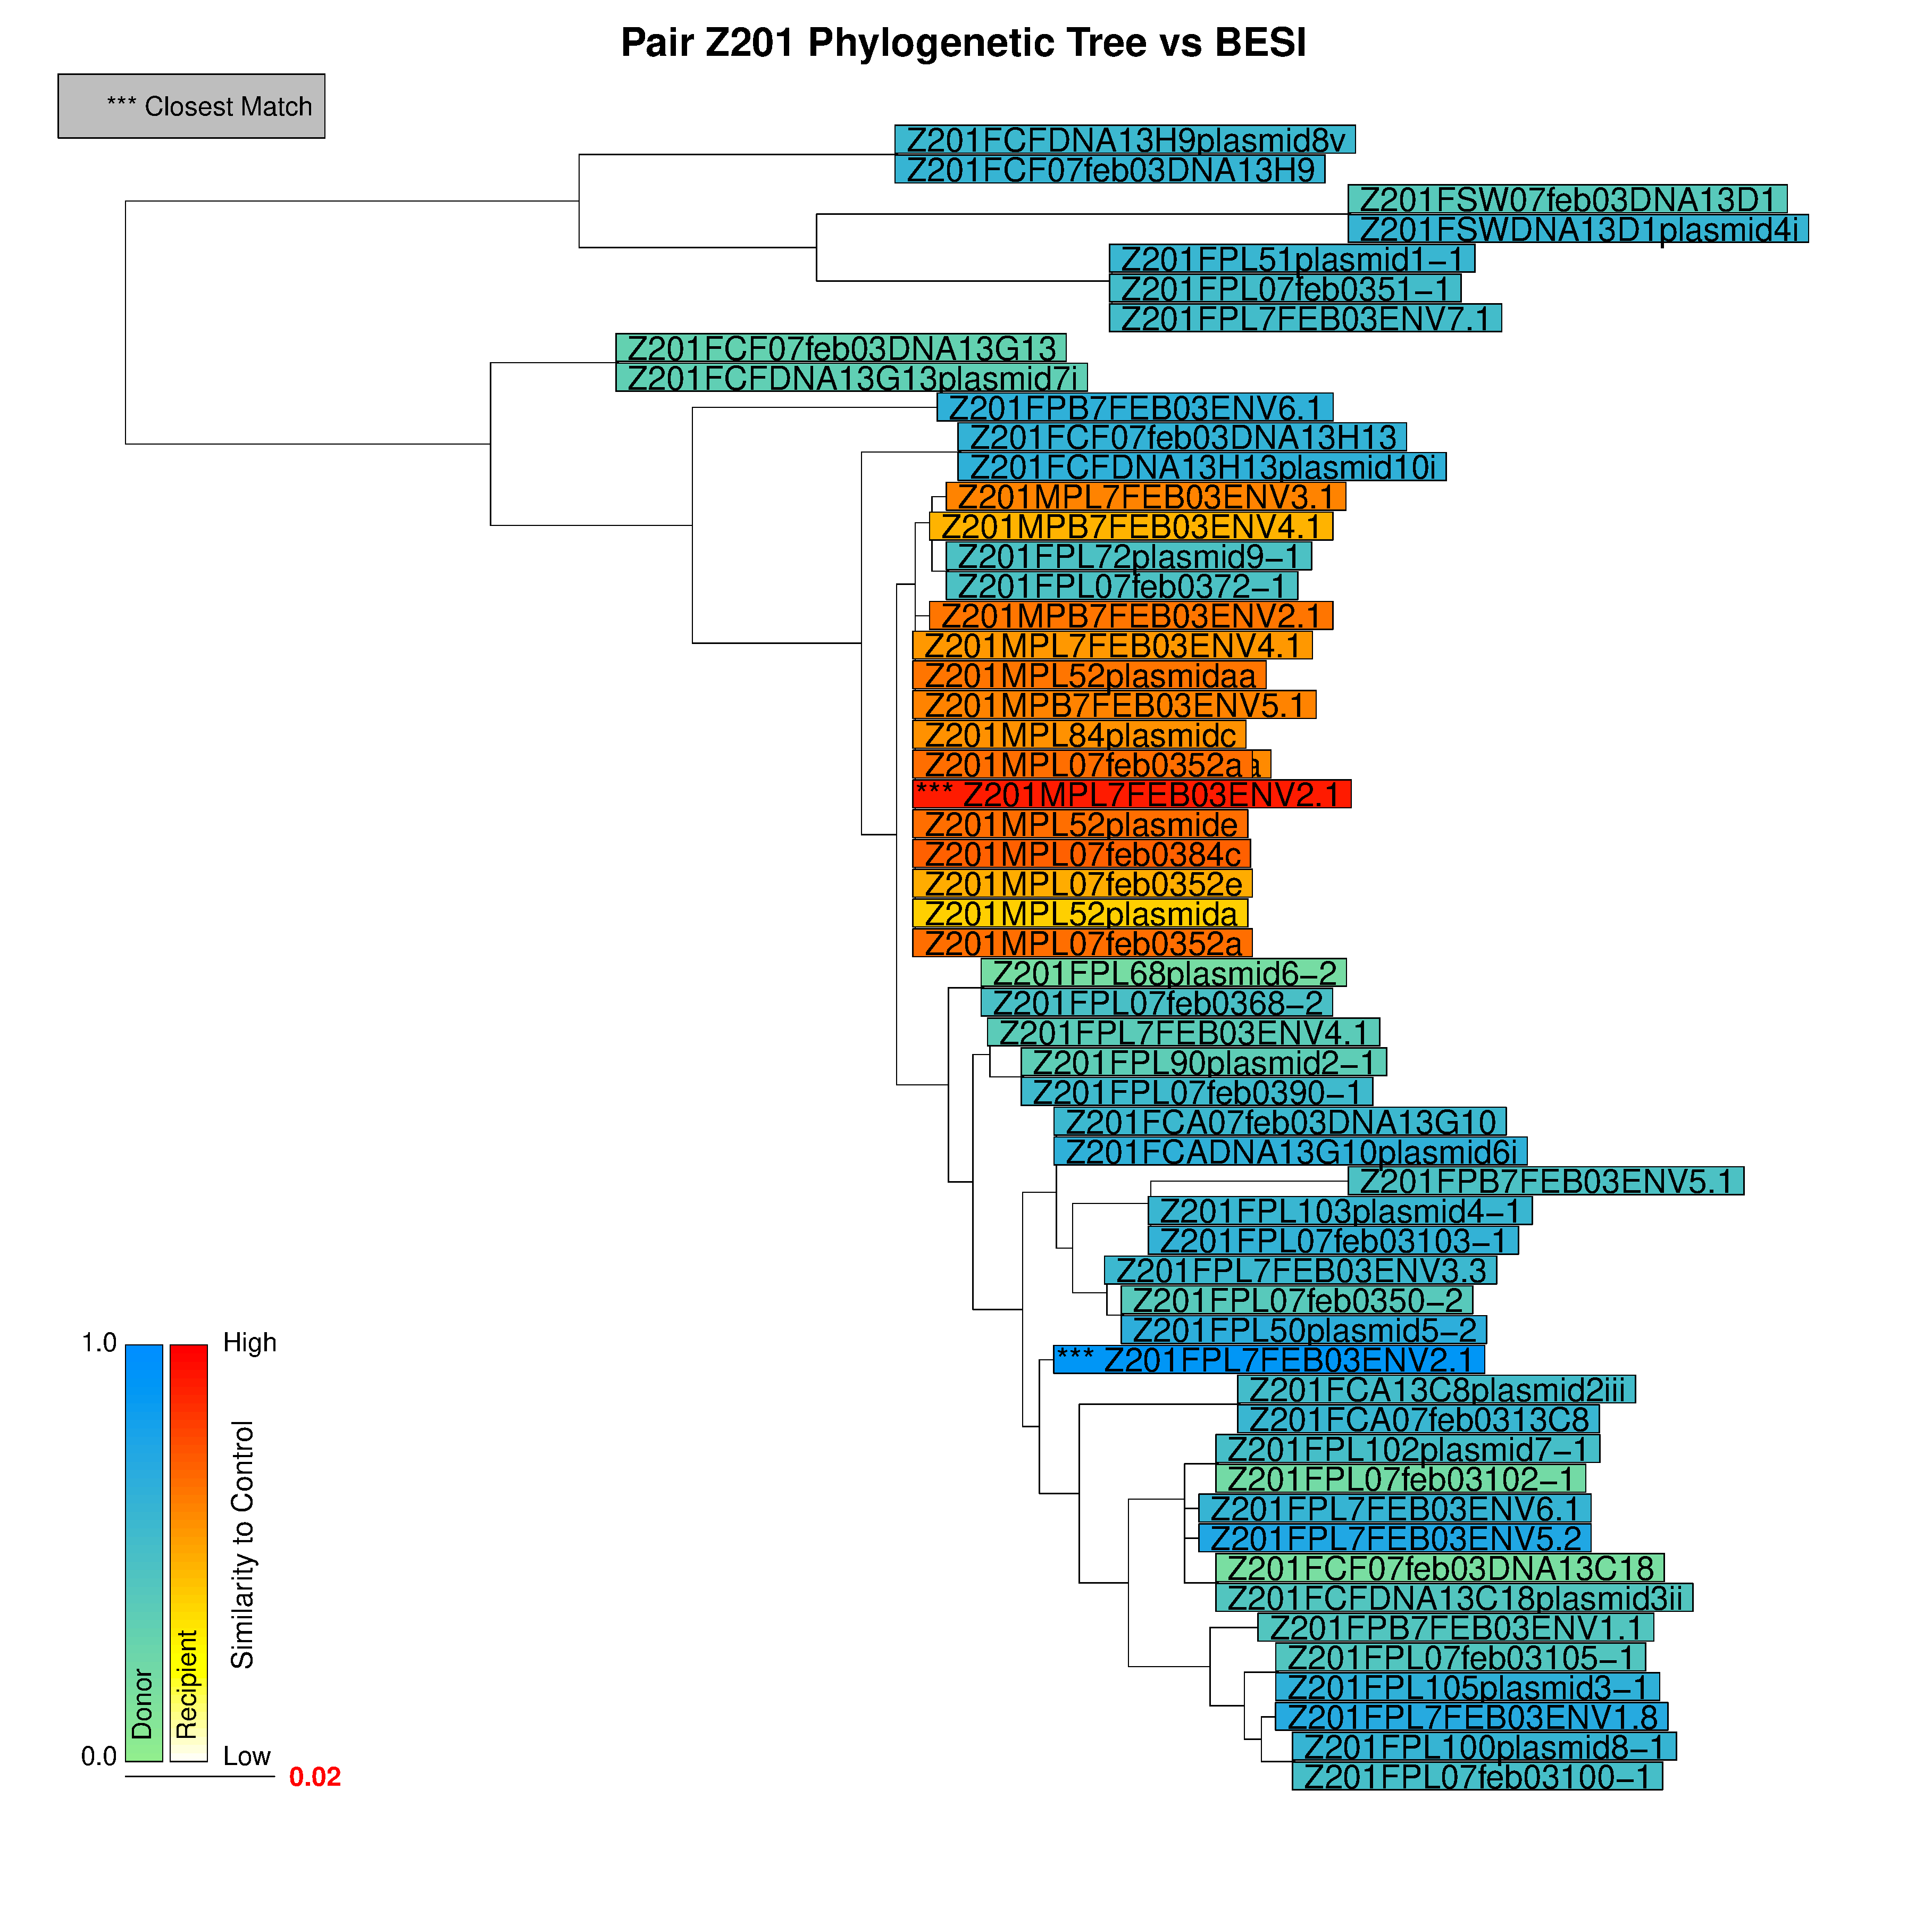
\includegraphics[width=\linewidth]{Z201_heat_map_Fixed-2}} 
\end{minipage}
&	\begin{tabular}{l l l}
	\textbf{Role} & \textbf{Sequence} & \textbf{Score}\\
	\hline
Donor &	Z201FCF07feb03DNA13C18	&	0.185587639941212	\\
&	Z201FPL68\_plasmid\_6-2	&	0.218424346755406	\\
&	Z201FPL07feb03102-1	&	0.223750622688585	\\
&	Z201FCF07feb03DNA13G13	&	0.327649913281141	\\
&	Z201FCFDNA13G13\_plasmid\_7i	&	0.356518526152355	\\
&	Z201FPL90\_plasmid\_2-1	&	0.375473898188648	\\
&	Z201FPL7FEB03ENV4.1	&	0.392372326811245	\\
&	Z201FSW07feb03DNA13D1	&	0.402796399343618	\\
&	Z201FPL07feb0350-2	&	0.409725055677222	\\
&	Z201FCFDNA13C18\_plasmid\_3ii	&	0.442345724467931	\\
&	Z201FPL07feb03105-1	&	0.442959887286871	\\
&	Z201FPB7FEB03ENV1.1	&	0.451253180056783	\\
&	Z201FPB7FEB03ENV5.1	&	0.48849051548773	\\
&	Z201FPL07feb0372-1	&	0.490956374815917	\\
&	Z201FPL72\_plasmid\_9-1	&	0.496684743422855	\\
&	Z201FPL07feb0368-2	&	0.513282753965808	\\
&	Z201FPL102\_plasmid\_7-1	&	0.521428901521057	\\
&	Z201FPL07feb03100-1	&	0.525412241308349	\\
&	Z201FPL7FEB03ENV7.1	&	0.54982676598373	\\
&	Z201FPL07feb0351-1	&	0.552025480983305	\\
&	Z201FCA13C8\_plasmid\_2iii	&	0.558488731618101	\\
&	Z201FPL07feb0390-1	&	0.561412545693259	\\
&	Z201FCFDNA13H9\_plasmid\_8v	&	0.58328804131525	\\
&	Z201FCA07feb03DNA13G10	&	0.585007632332971	\\
&	Z201FPL7FEB03ENV3.3	&	0.597020412406579	\\
&	Z201FCA07feb0313C8	&	0.600254757869134	\\
&	Z201FPL51\_plasmid\_1-1	&	0.606156319414256	\\
&	Z201FPL103\_plasmid\_4-1	&	0.618089893764309	\\
&	Z201FCF07feb03DNA13H9	&	0.621896669668123	\\
&	Z201FSWDNA13D1\_plasmid\_4i	&	0.622783049486914	\\
&	Z201FPL7FEB03ENV6.1	&	0.623900465916333	\\
&	Z201FPL100\_plasmid\_8-1	&	0.638588866111133	\\
&	Z201FCF07feb03DNA13H13	&	0.640034289023372	\\
&	Z201FPL07feb03103-1	&	0.640428862459292	\\
&	Z201FPB7FEB03ENV6.1	&	0.666460329841705	\\
&	Z201FCADNA13G10\_plasmid\_6i	&	0.667537281351855	\\
&	Z201FCFDNA13H13\_plasmid\_10i	&	0.672811878537835	\\
&	Z201FPL105\_plasmid\_3-1	&	0.677789985861925	\\
&	Z201FPL50\_plasmid\_5-2	&	0.698393129335323	\\
&	Z201FPL7FEB03ENV1.8	&	0.729943557404322	\\
&	Z201FPL7FEB03ENV5.2	&	0.77205029057402	\\
&	Z201FPL7FEB03ENV2.1	&	0.937733719093409	\\

	& \ &\ \\
	\hline
Recipient &	Z201MPL52\_plasmid\_a	&	0.405501457711246	\\
&	Z201MPB7FEB03ENV4.1	&	0.49164733067342	\\
&	Z201MPL07feb0352e	&	0.511660996776478	\\
&	Z201MPL7FEB03ENV4.1	&	0.564077491743853	\\
&	Z201MPL84\_plasmid\_c	&	0.596445551627584	\\
&	Z201MPL07feb0352aa	&	0.616971843958095	\\
&	Z201MPL7FEB03ENV3.1	&	0.637822939727832	\\
&	Z201MPB7FEB03ENV5.1	&	0.639699539360303	\\
&	Z201MPB7FEB03ENV2.1	&	0.665309510264914	\\
&	Z201MPL52\_plasmid\_aa	&	0.671428047818562	\\
&	Z201MPL07feb0352a	&	0.68649647736828	\\
&	Z201MPL52\_plasmid\_e	&	0.699811465012657	\\
&	Z201MPL07feb0384c	&	0.726611622441189	\\
&	Z201MPL7FEB03ENV2.1	&	0.921195312318658	\\

\end{tabular}\\
\hline
& \ \\
\begin{minipage}{.4\textwidth}
	\raisebox{-\totalheight}{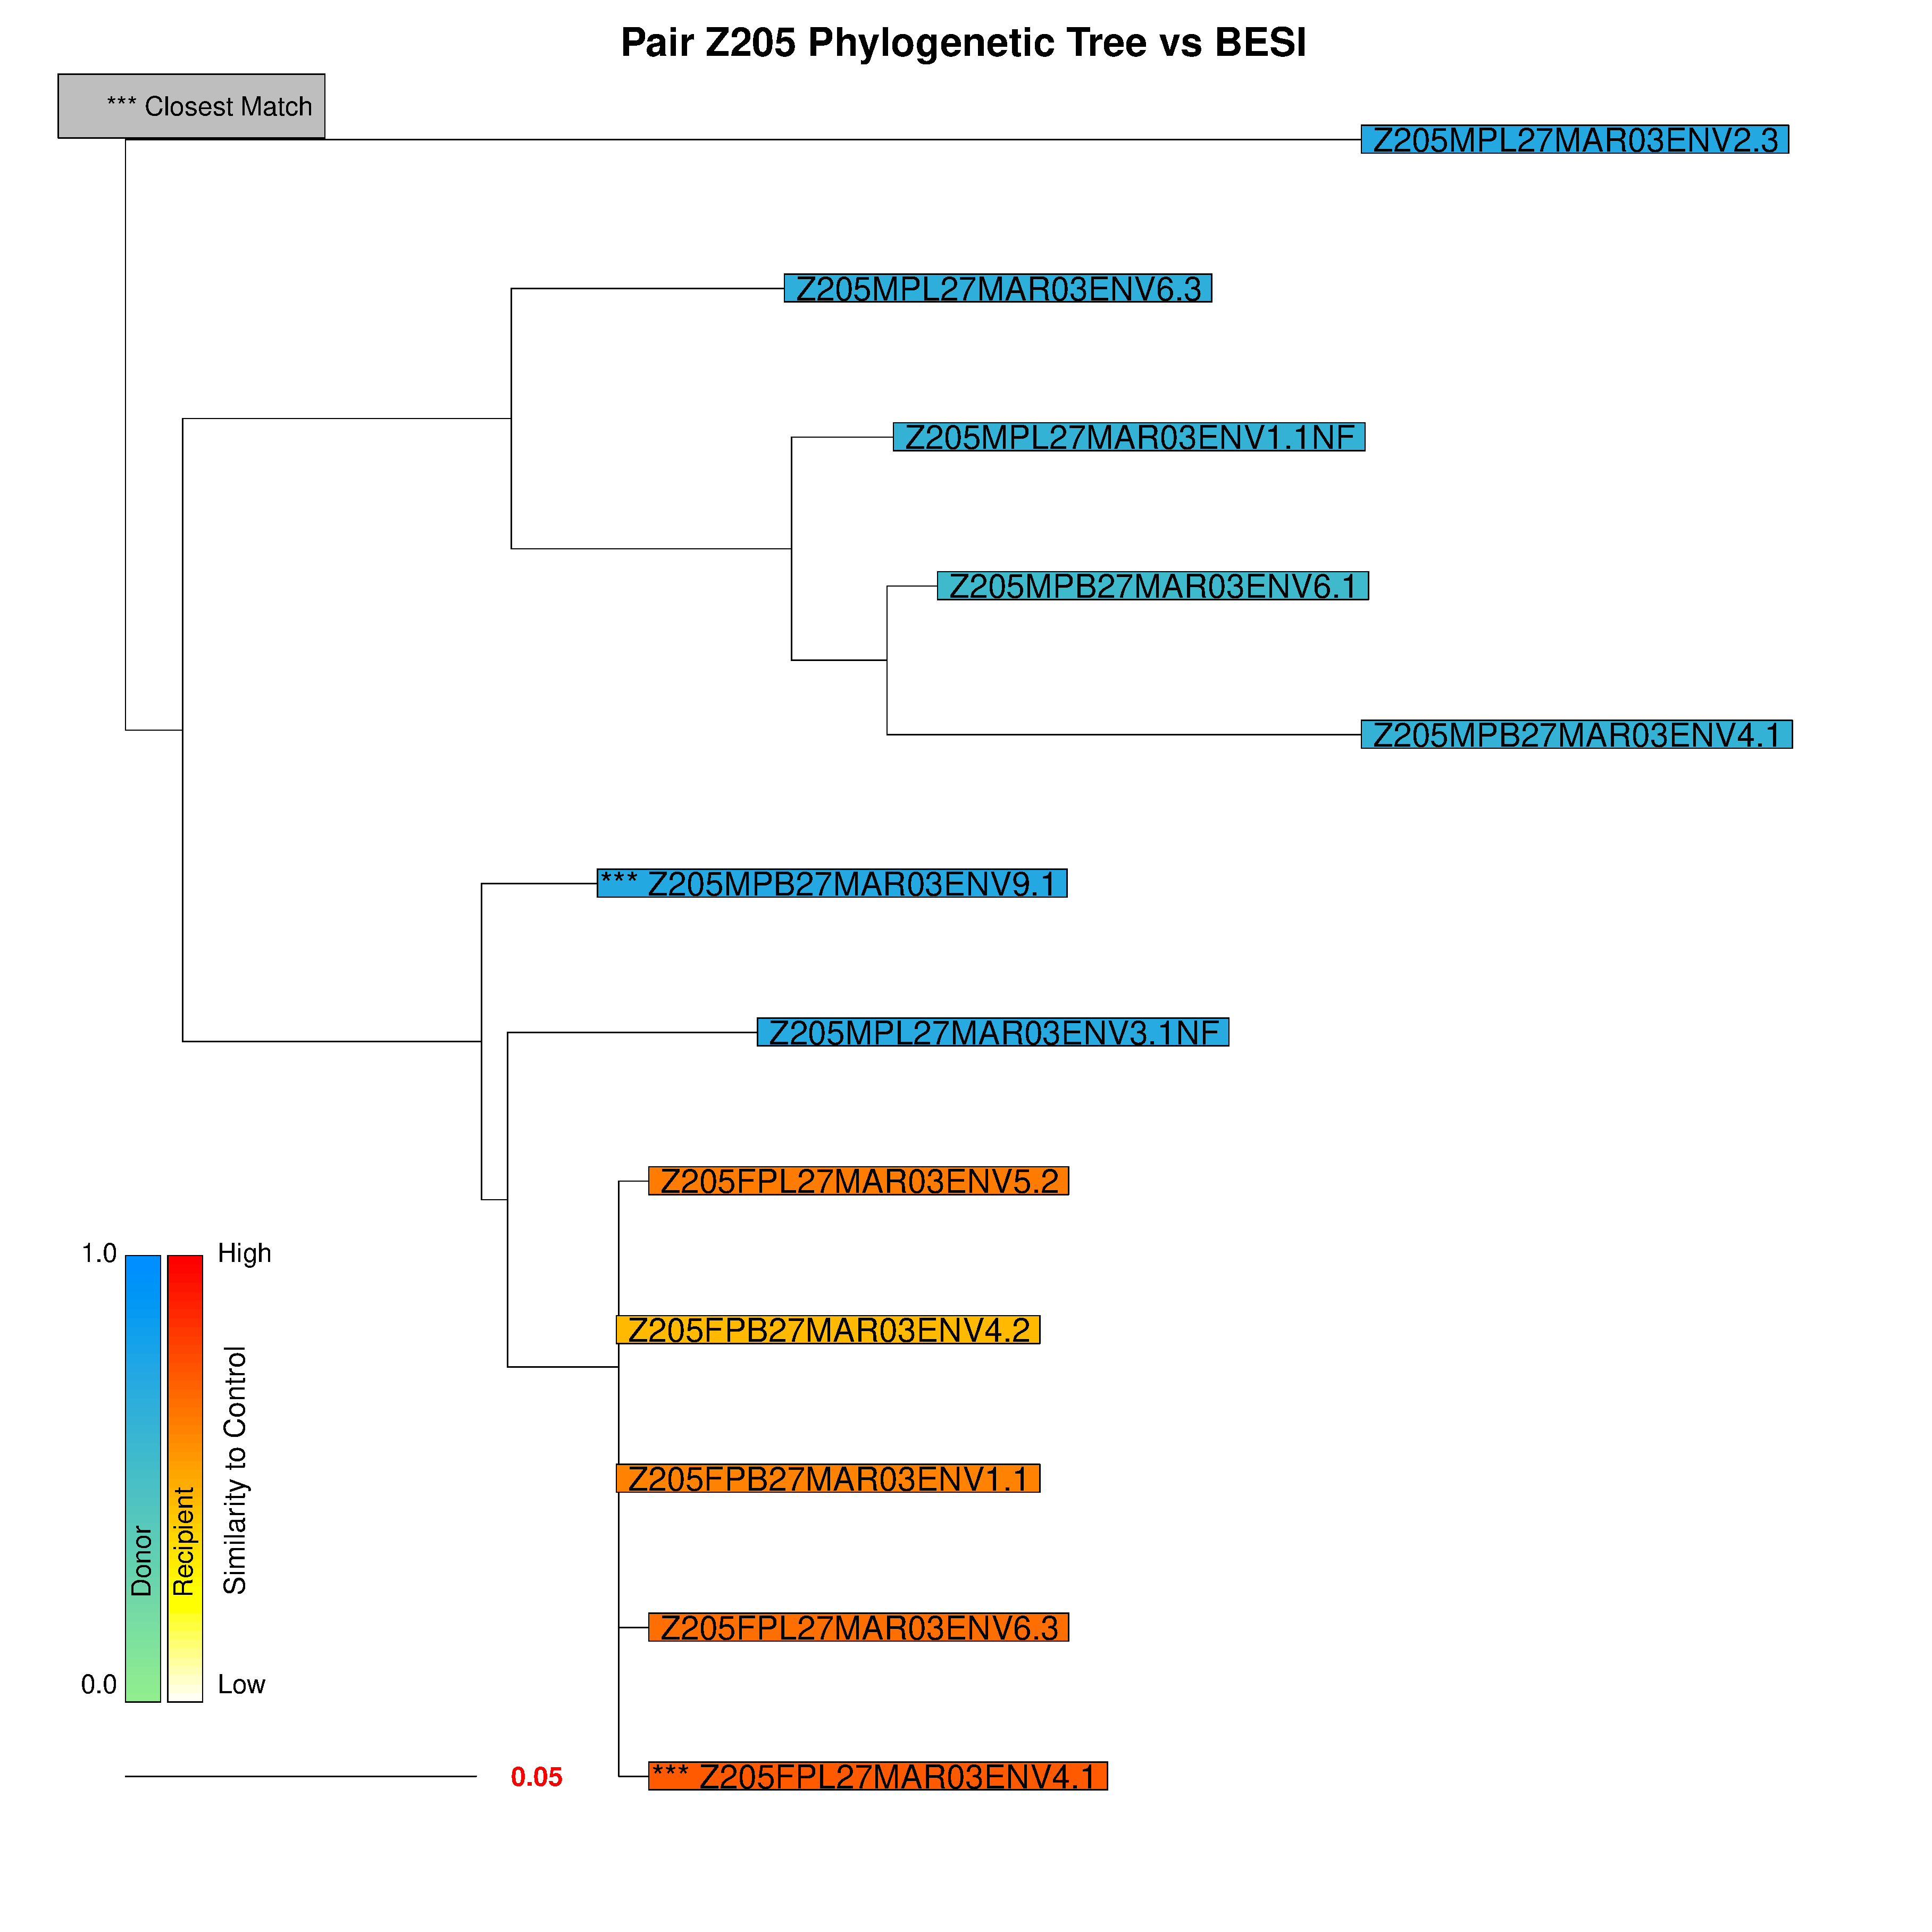
\includegraphics[width=\linewidth]{Z205_heat_map_Fixed-2}} 
\end{minipage}
&	\begin{tabular}{l l l}
	\textbf{Role} & \textbf{Sequence} & \textbf{Score}\\
	\hline
Recipient &	Z205FPB27MAR03ENV4.2	&	0.462208304982716	\\
&	Z205FPB27MAR03ENV1.1	&	0.628243173867313	\\
&	Z205FPL27MAR03ENV5.2	&	0.649421585875164	\\
&	Z205FPL27MAR03ENV6.3	&	0.682783813315067	\\
&	Z205FPL27MAR03ENV4.1	&	0.74237902312304	\\

	& \ &\ \\
	\hline
Donor &	Z205MPB27MAR03ENV6.1	&	0.576458537237502	\\
&	Z205MPL27MAR03ENV1.1NF	&	0.647225092379855	\\
&	Z205MPB27MAR03ENV4.1	&	0.657645194881687	\\
&	Z205MPL27MAR03ENV6.3	&	0.691913445086819	\\
&	Z205MPL27MAR03ENV3.1NF	&	0.735715823607924	\\
&	Z205MPL27MAR03ENV2.3	&	0.740710281975924	\\
&	Z205MPB27MAR03ENV9.1	&	0.750062534639445	\\

\end{tabular}\\
\end{tabular}
\end{table*}

\begin{table*}[]
	\begin{tabular}{ c c}
\begin{minipage}{.4\textwidth}
	\raisebox{-\totalheight}{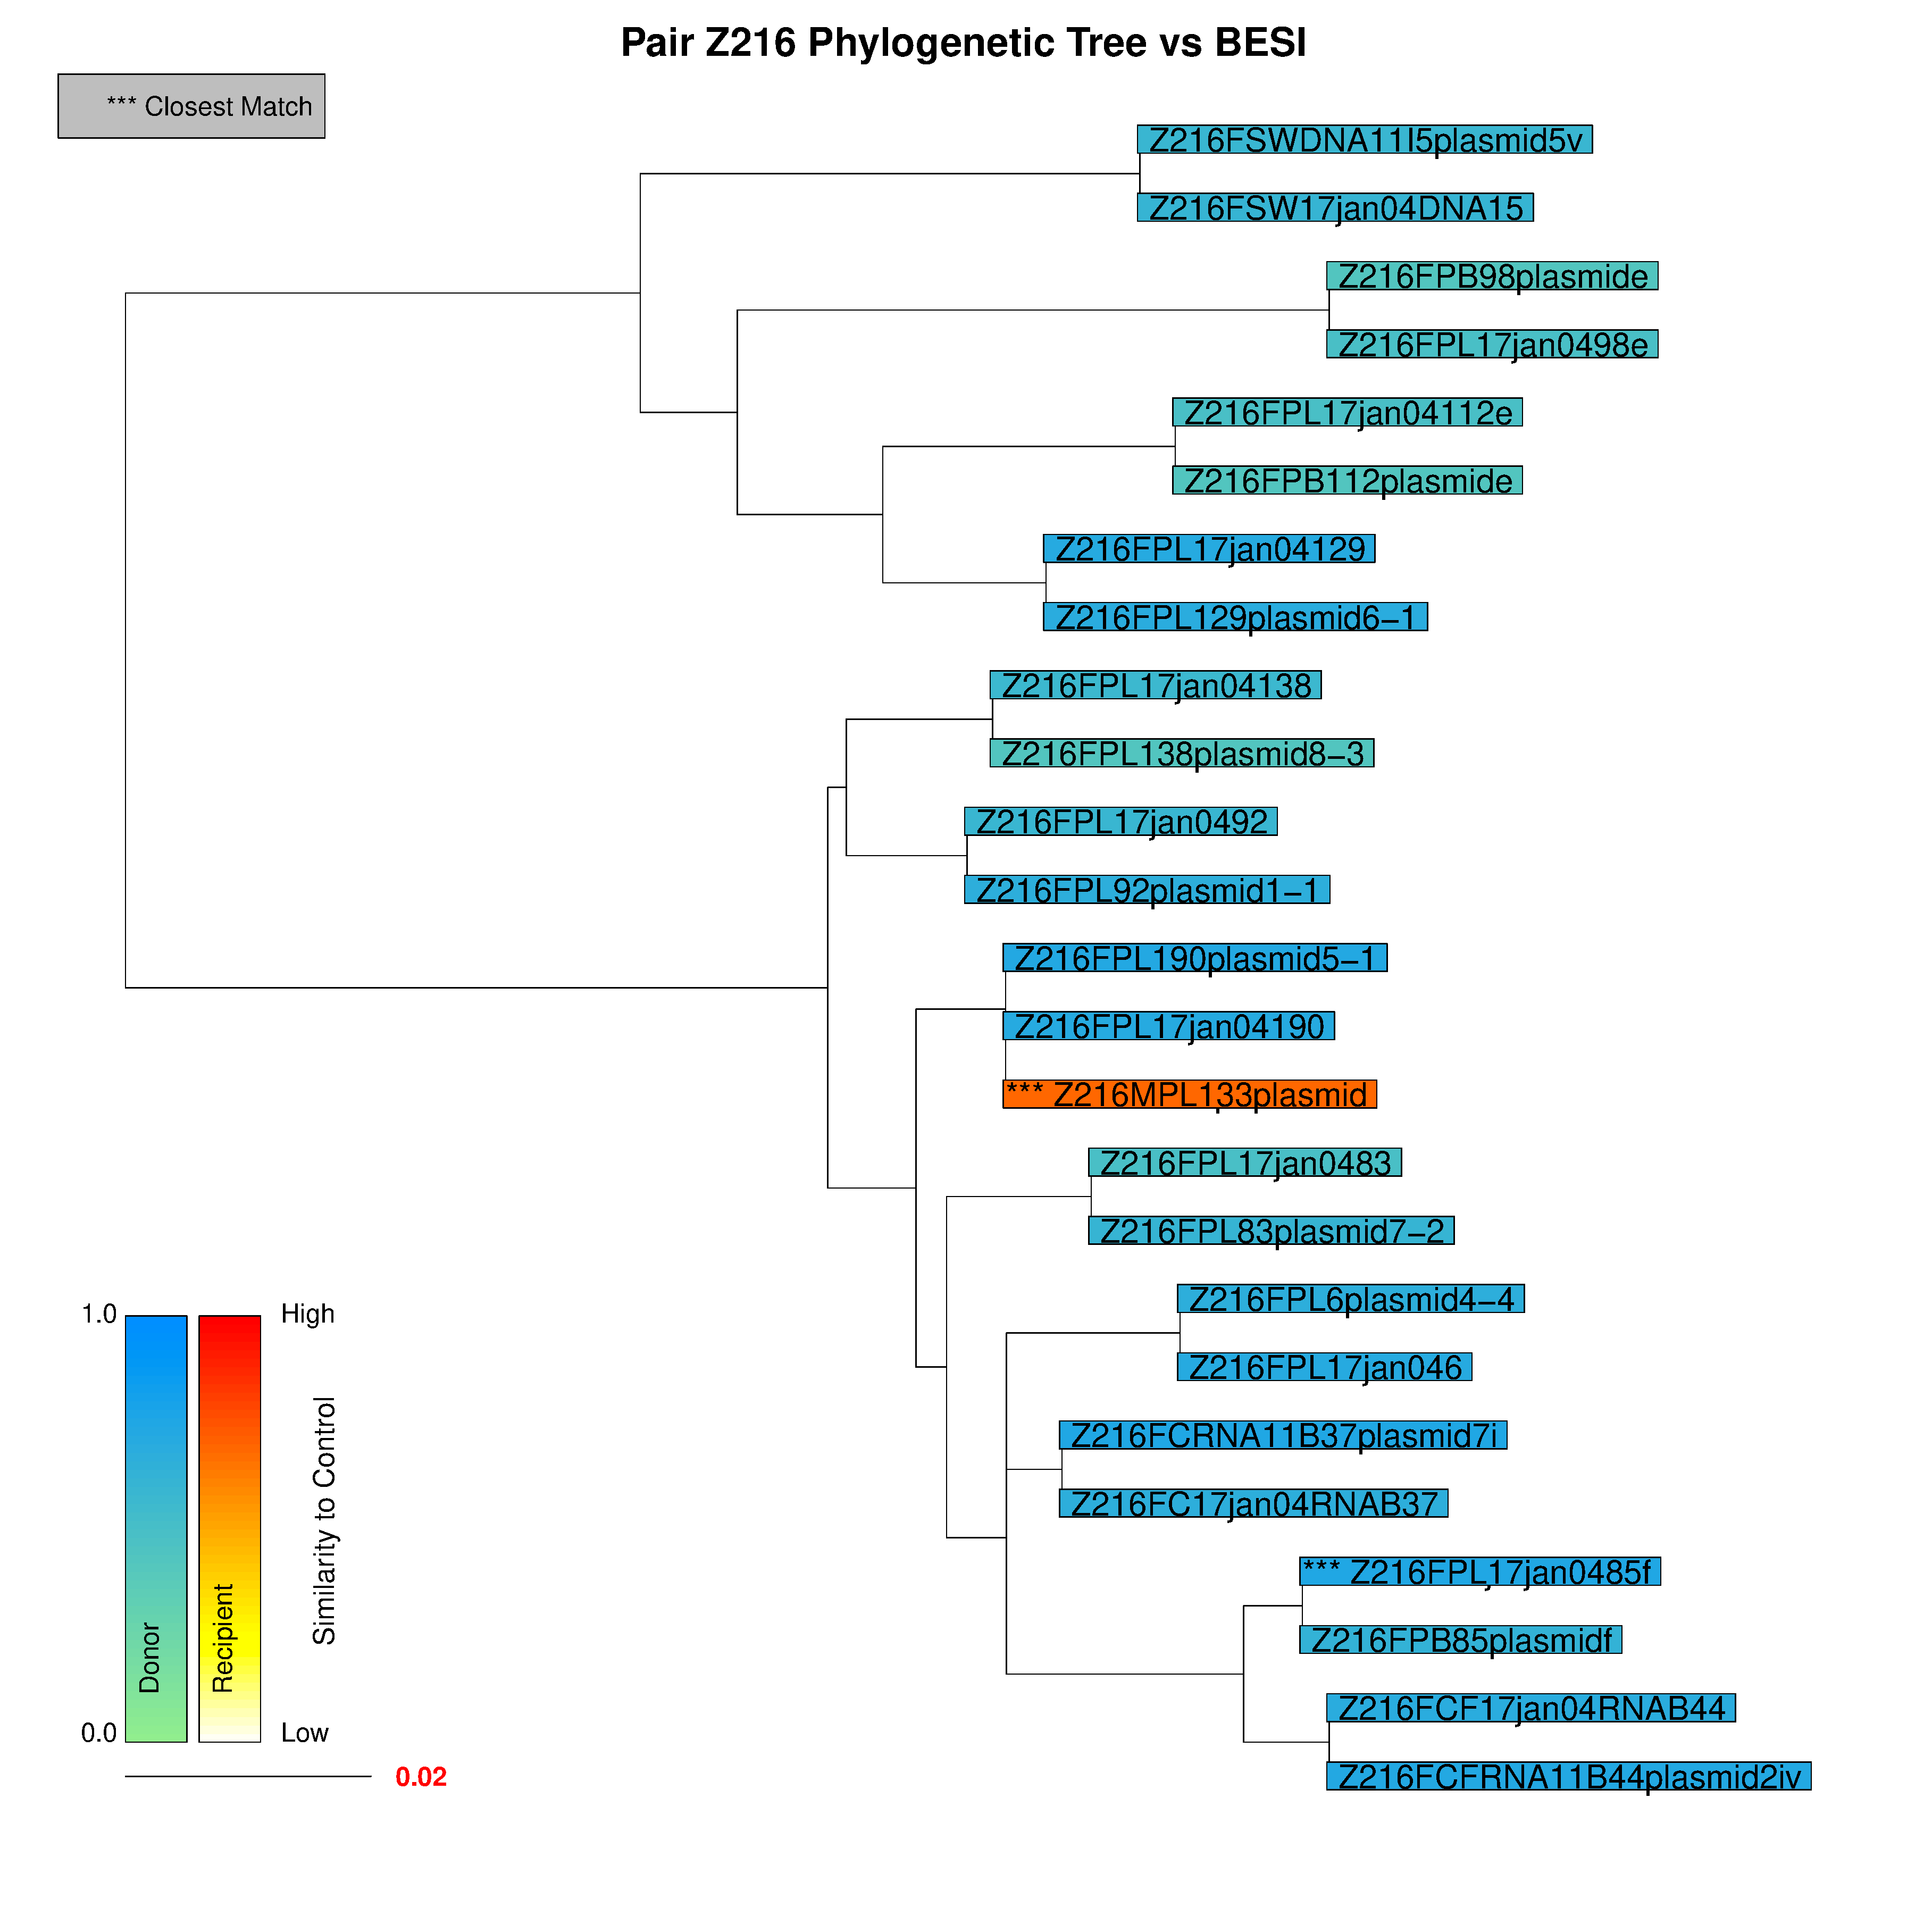
\includegraphics[width=\linewidth]{Z216_heat_map_Fixed-2}} 
\end{minipage}
&	\begin{tabular}{l l l}
	\textbf{Role} & \textbf{Sequence} & \textbf{Score}\\
	\hline
Donor &	Z216FPB98\_plasmid\_e	&	0.443137527302722	\\
&	Z216FPL138\_plasmid\_8-3	&	0.449525104124591	\\
&	Z216FPB112\_plasmid\_e	&	0.458509279022854	\\
&	Z216FPL17jan04112e	&	0.509027672053639	\\
&	Z216FPL17jan0498e	&	0.511841025065402	\\
&	Z216FPL17jan0483	&	0.518916798560644	\\
&	Z216FPL17jan04138	&	0.581988997367823	\\
&	Z216FSWDNA11I5\_plasmid\_5v	&	0.604127778489093	\\
&	Z216FPL17jan0492	&	0.605354960442271	\\
&	Z216FSW17jan04DNA15	&	0.621360888228847	\\
&	Z216FPL83\_plasmid\_7-2	&	0.62445496799261	\\
&	Z216FPB85\_plasmid\_f	&	0.649648082586884	\\
&	Z216FC17jan04RNAB37	&	0.685767887559145	\\
&	Z216FPL6\_plasmid\_4-4	&	0.697066484072342	\\
&	Z216FPL92\_plasmid\_1-1	&	0.699855447182106	\\
&	Z216FCF17jan04RNAB44	&	0.702529418440598	\\
&	Z216FPL129\_plasmid\_6-1	&	0.703196634247862	\\
&	Z216FPL17jan04190	&	0.729998827272817	\\
&	Z216FPL17jan04129	&	0.730563294379777	\\
&	Z216FPL17jan046	&	0.730797187023113	\\
&	Z216FPL190\_plasmid\_5-1	&	0.742086473318316	\\
&	Z216FCFRNA11B44\_plasmid\_2iv	&	0.759464572677266	\\
&	Z216FCRNA11B37\_plasmid\_7i	&	0.764963184767281	\\
&	Z216FPL17jan0485f	&	0.776617270079055	\\

	& \ &\ \\
	\hline
Recipient &	Z216MPL133\_plasmid	&	0.703005915889016	\\

\end{tabular}\\
\hline
& \ \\
\begin{minipage}{.4\textwidth}
	\raisebox{-\totalheight}{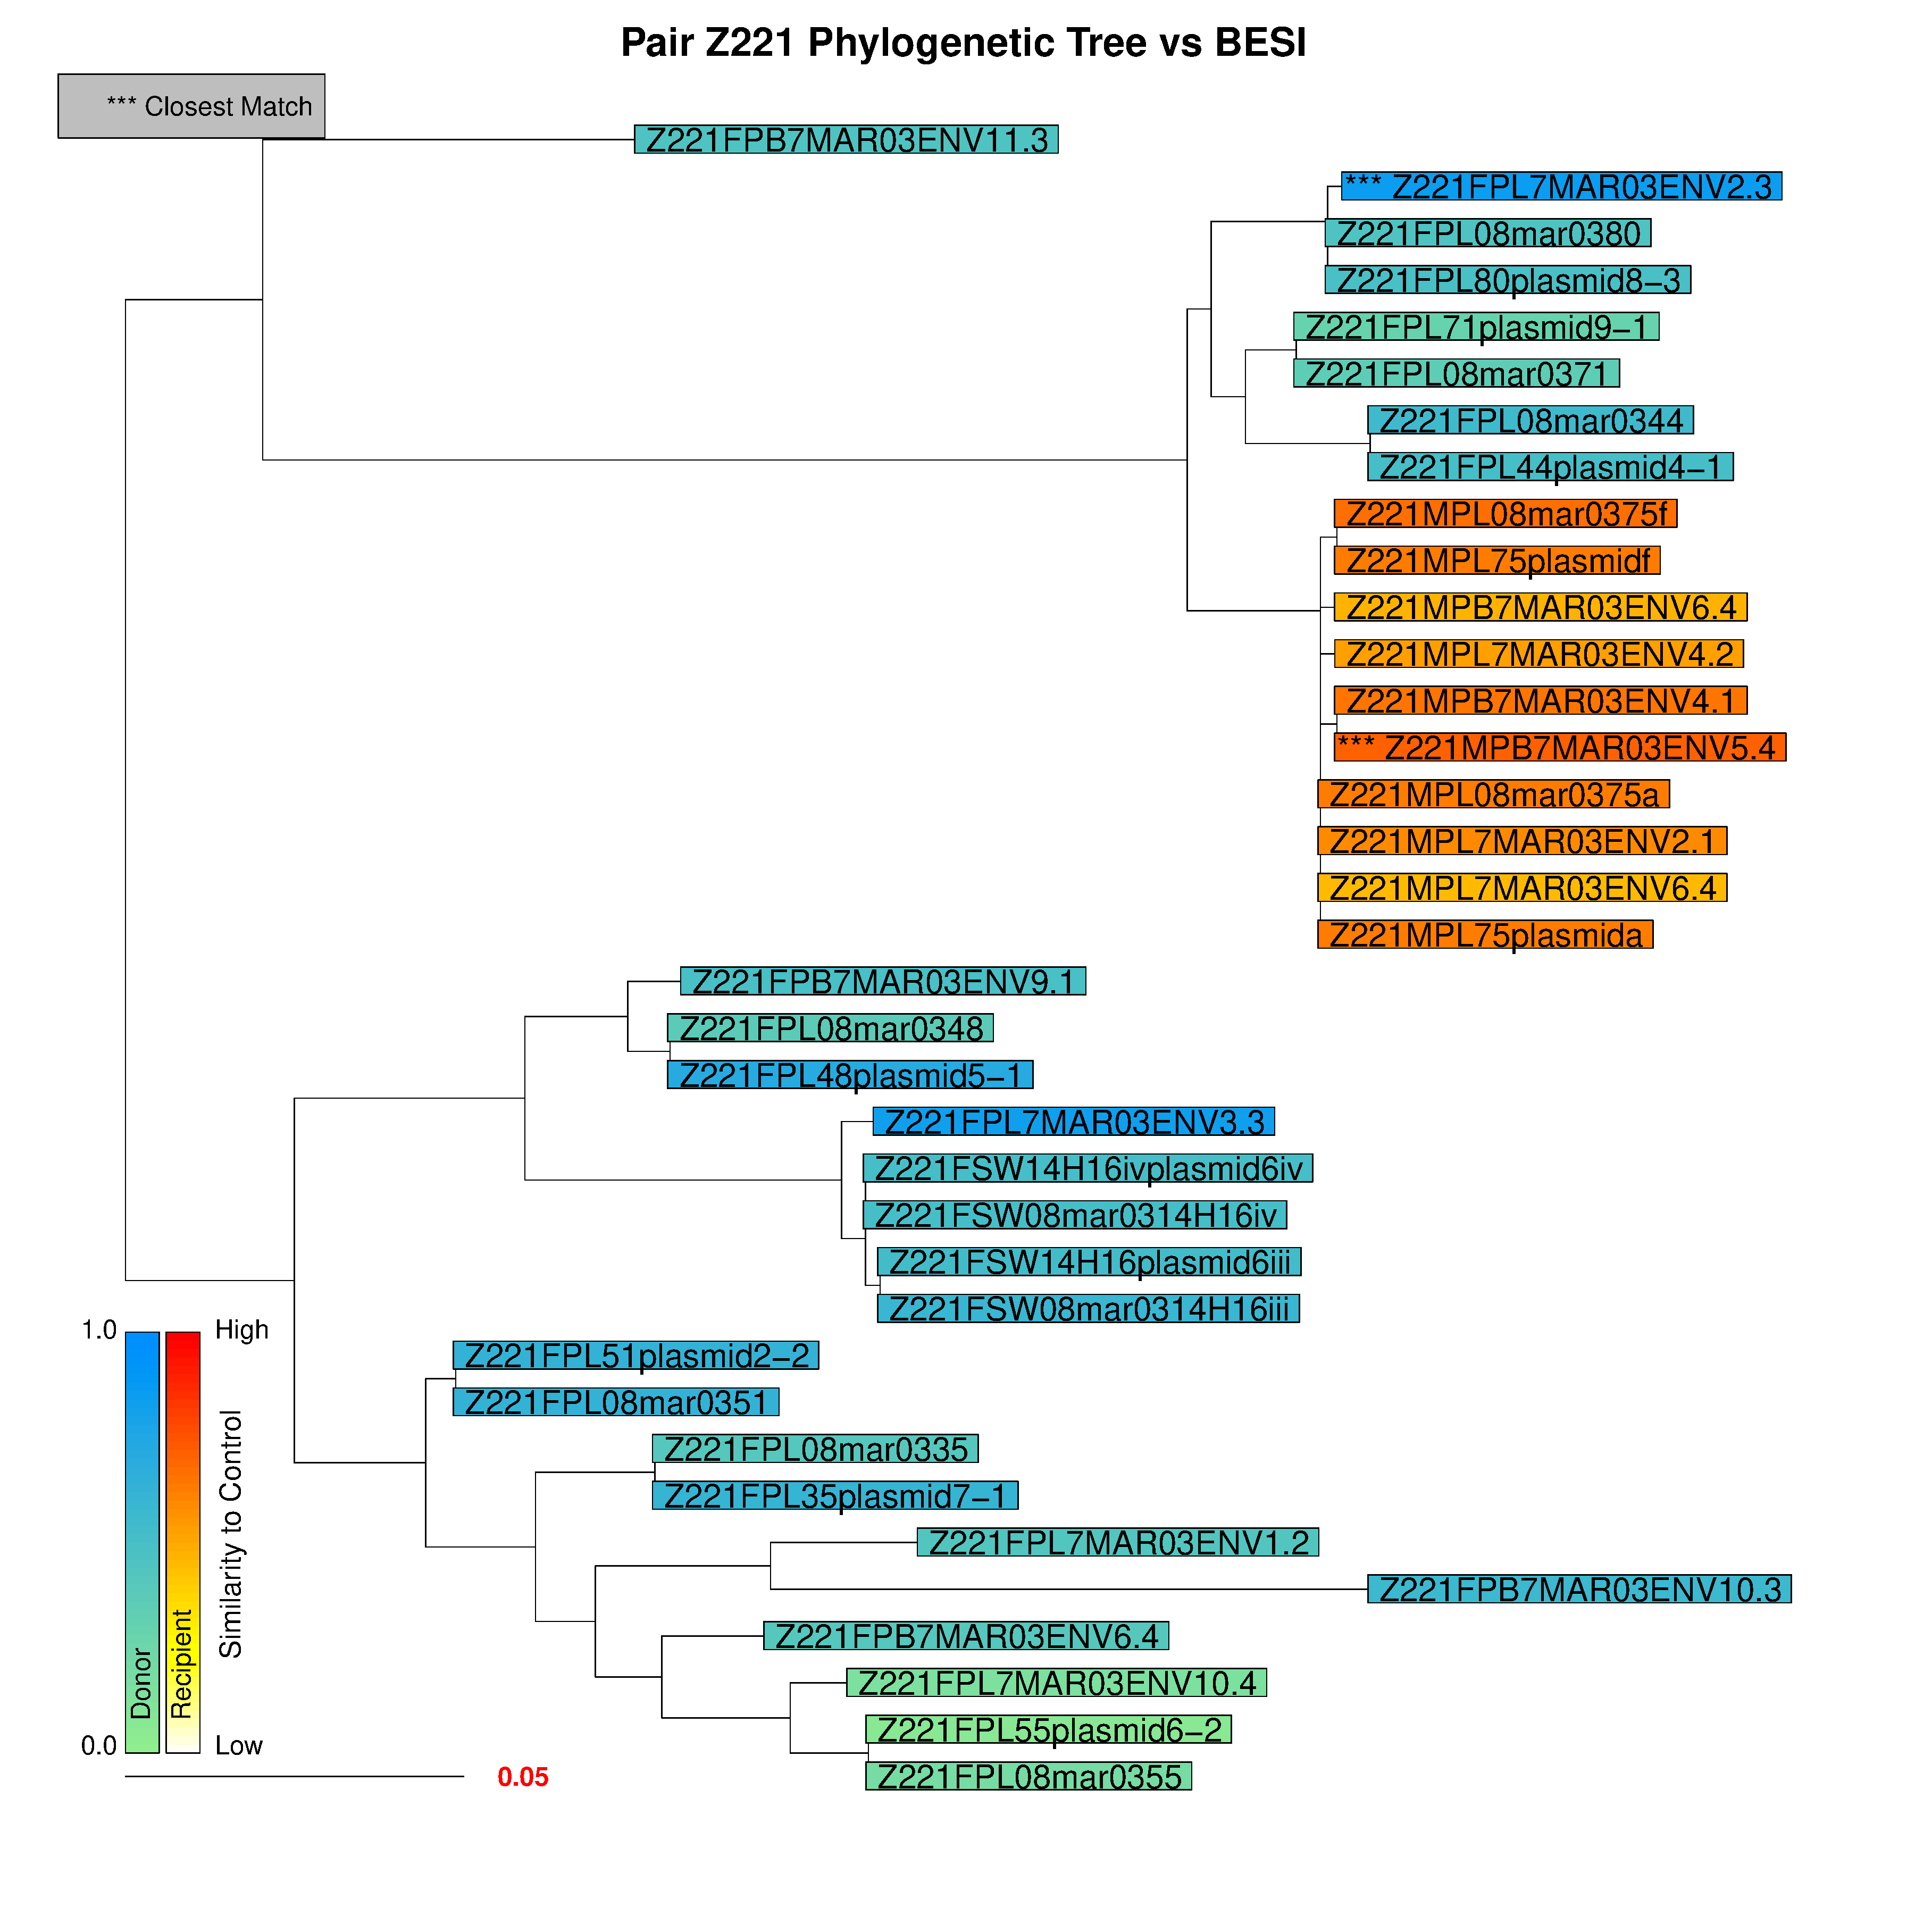
\includegraphics[width=\linewidth]{Z221_heat_map_Fixed-2}} 
\end{minipage}
&	\begin{tabular}{l l l}
	\textbf{Role} & \textbf{Sequence} & \textbf{Score}\\
	\hline
Donor &	Z221FPL55\_plasmid\_6-2	&	0.088284202030072	\\
&	Z221FPL7MAR03ENV10.4	&	0.171490857115365	\\
&	Z221FPL08mar0355	&	0.204711706842976	\\
&	Z221FPL71\_plasmid\_9-1	&	0.313781268259494	\\
&	Z221FPL08mar0371	&	0.36479808138766	\\
&	Z221FPL08mar0348	&	0.380170329339289	\\
&	Z221FPL08mar0335	&	0.423973605336986	\\
&	Z221FPB7MAR03ENV6.4	&	0.434531640214774	\\
&	Z221FPL7MAR03ENV1.2	&	0.444789811935412	\\
&	Z221FPL08mar0380	&	0.461477509411852	\\
&	Z221FPB7MAR03ENV11.3	&	0.463830898489805	\\
&	Z221FPL80\_plasmid\_8-3	&	0.500014648026271	\\
&	Z221FPB7MAR03ENV9.1	&	0.50744726000043	\\
&	Z221FPL44\_plasmid\_4-1	&	0.520886155816621	\\
&	Z221FSW14H16iv\_plasmid\_6iv	&	0.520993779335181	\\
&	Z221FSW08mar0314H16iv	&	0.530733903452594	\\
&	Z221FSW14H16\_plasmid\_6iii	&	0.558116171482779	\\
&	Z221FPL08mar0344	&	0.567419858400105	\\
&	Z221FPB7MAR03ENV10.3	&	0.597044012834383	\\
&	Z221FSW08mar0314H16iii	&	0.618385614501745	\\
&	Z221FPL35\_plasmid\_7-1	&	0.625798429940925	\\
&	Z221FPL51\_plasmid\_2-2	&	0.652299448655206	\\
&	Z221FPL08mar0351	&	0.654528149289713	\\
&	Z221FPL48\_plasmid\_5-1	&	0.725035258721497	\\
&	Z221FPL7MAR03ENV3.3	&	0.844043108854056	\\
&	Z221FPL7MAR03ENV2.3	&	0.869016547898083	\\

	& \ &\ \\
	\hline
Recipient &	Z221MPL7MAR03ENV6.4	&	0.460299657849798	\\
&	Z221MPB7MAR03ENV6.4	&	0.494879066406671	\\
&	Z221MPL7MAR03ENV4.2	&	0.559573703682982	\\
&	Z221MPL7MAR03ENV2.1	&	0.614062275947335	\\
&	Z221MPL08mar0375a	&	0.647772496706598	\\
&	Z221MPL75\_plasmid\_f	&	0.64783714507966	\\
&	Z221MPL75\_plasmid\_a	&	0.657000778355033	\\
&	Z221MPB7MAR03ENV4.1	&	0.678762348486901	\\
&	Z221MPL08mar0375f	&	0.681145585698272	\\
&	Z221MPB7MAR03ENV5.4	&	0.731790667812565	\\

\end{tabular}\\
\end{tabular}
\end{table*}

\begin{table*}[]
	\begin{tabular}{ c c}

\begin{minipage}{.4\textwidth}
	\raisebox{-\totalheight}{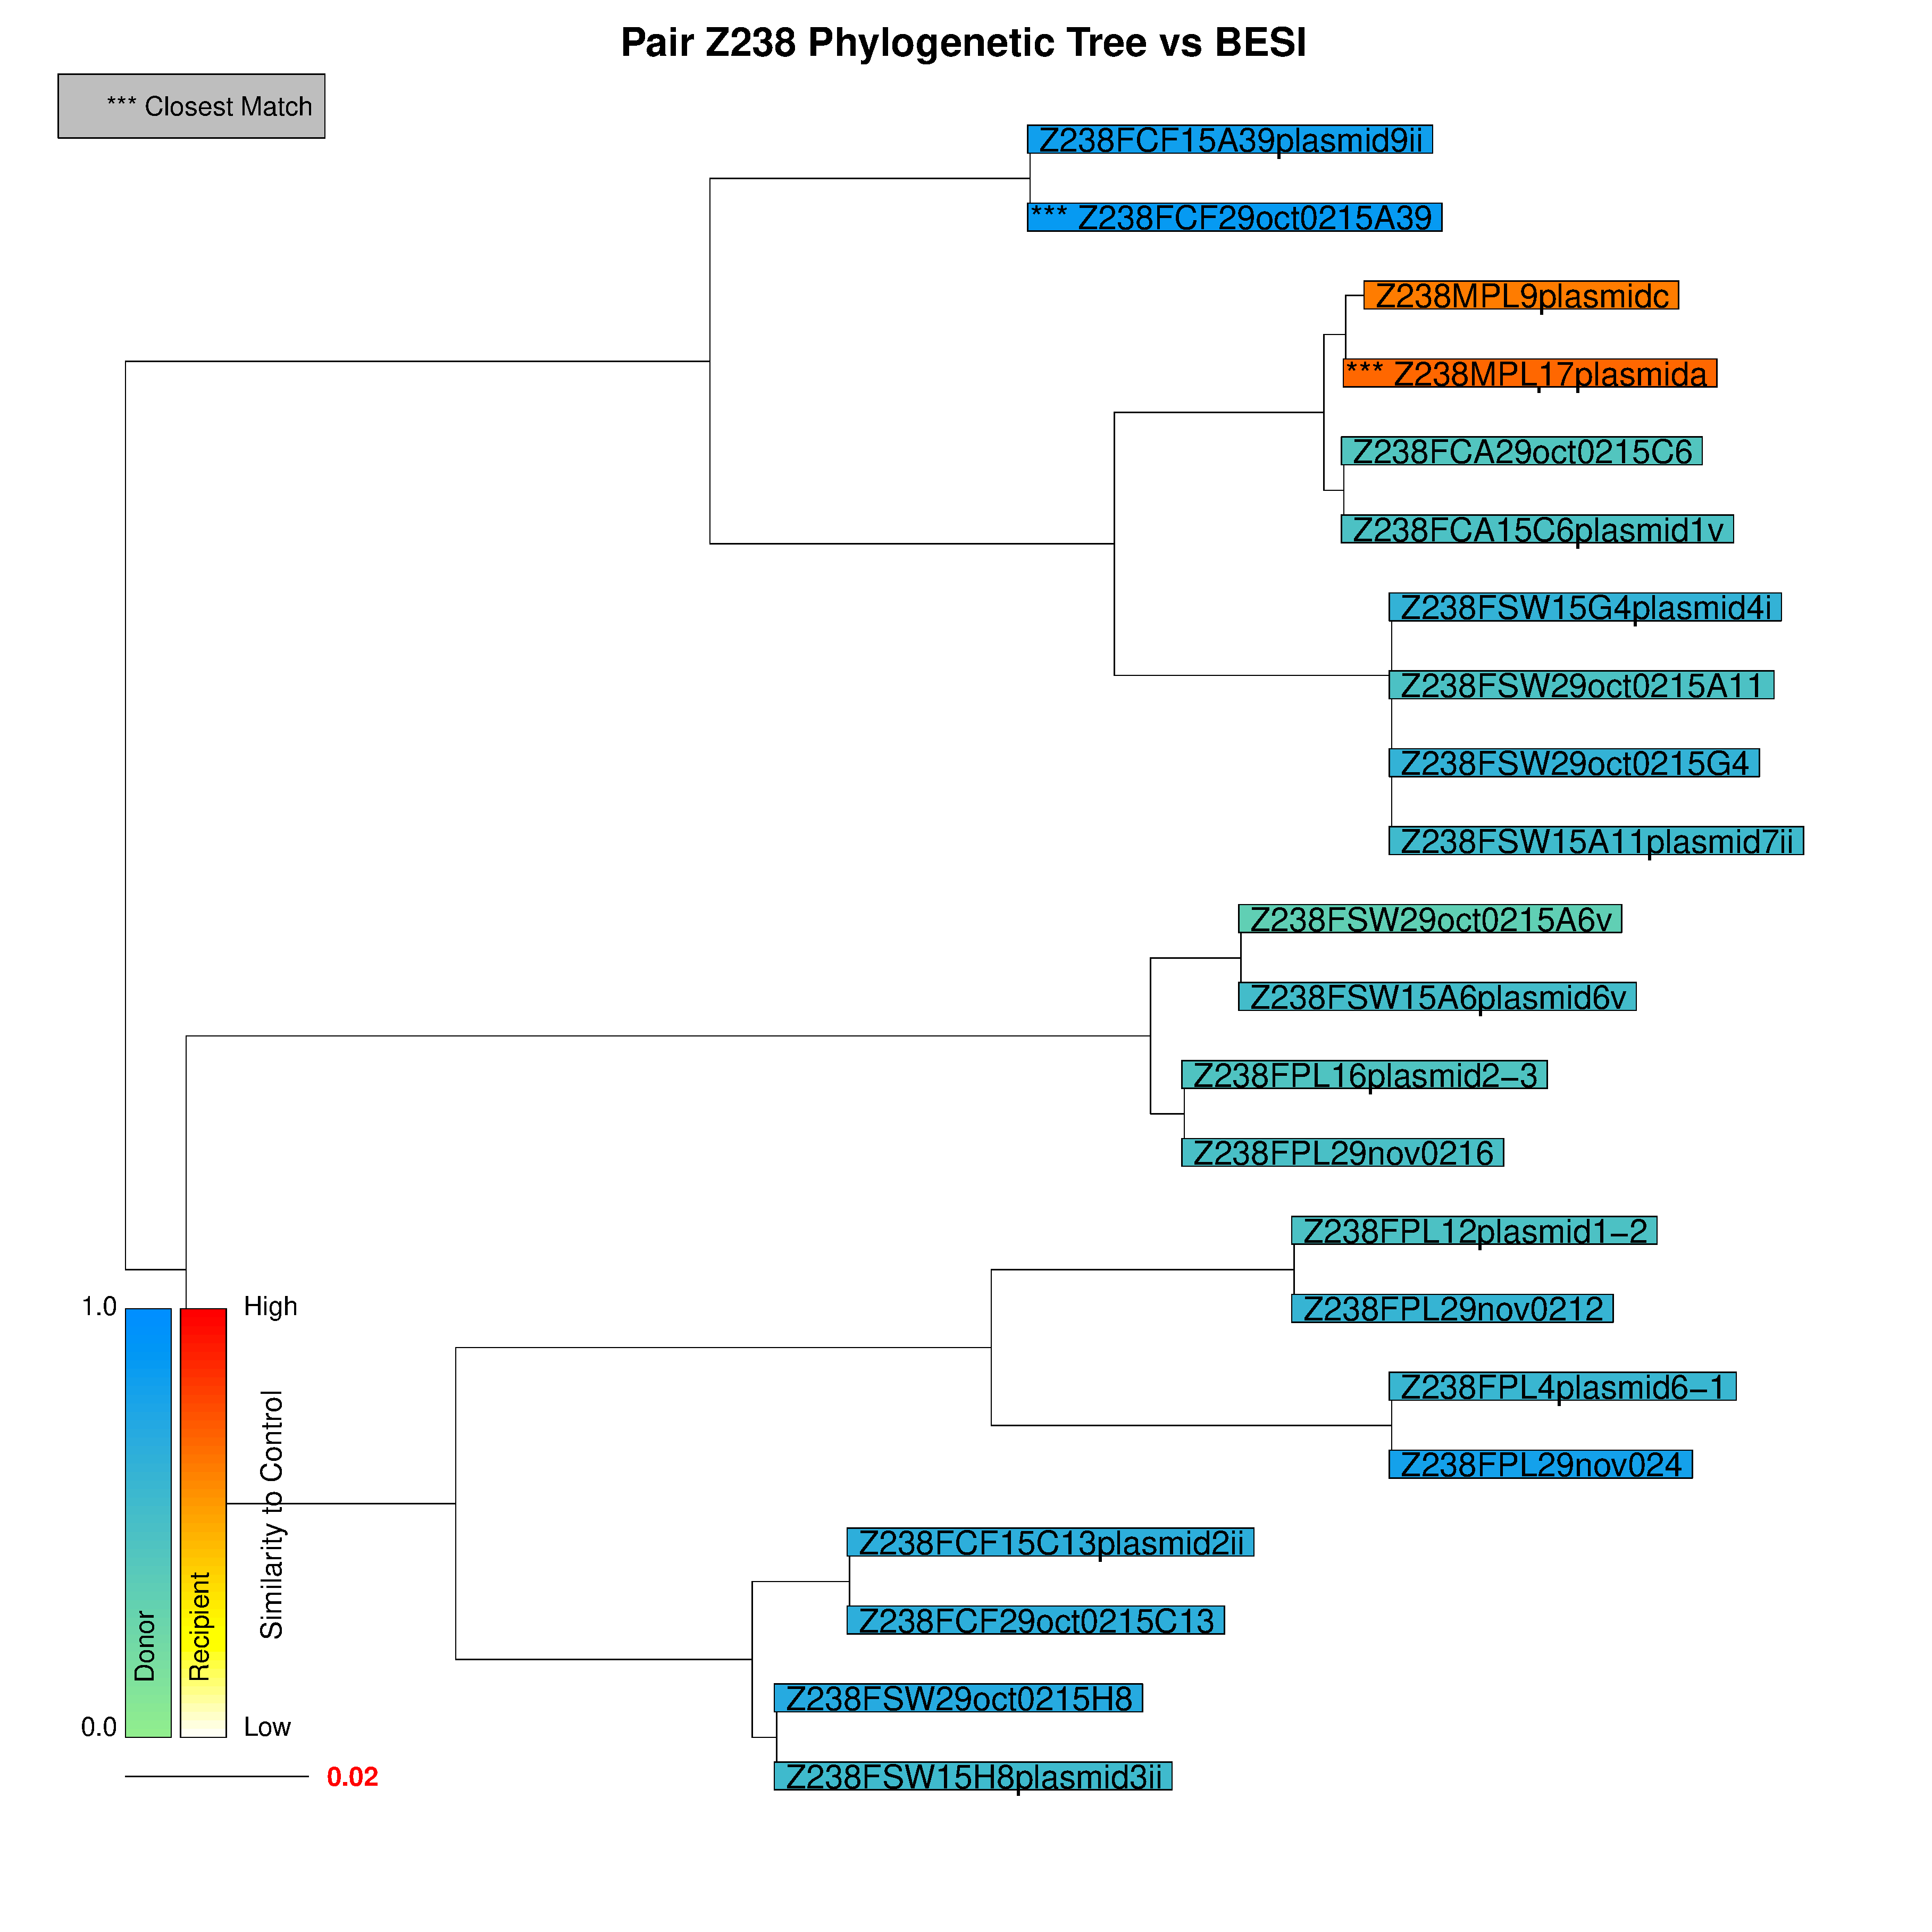
\includegraphics[width=\linewidth]{Z238_heat_map_Fixed-2}} 
\end{minipage}
&	\begin{tabular}{l l l}
	\textbf{Role} & \textbf{Sequence} & \textbf{Score}\\
	\hline
Donor &	Z238FSW29oct0215A6v	&	0.351697287784035	\\
&	Z238FCA29oct0215C6	&	0.451600093908692	\\
&	Z238FPL16\_plasmid\_2-3	&	0.463870251207422	\\
&	Z238FSW29oct0215A11	&	0.483797710578397	\\
&	Z238FPL12\_plasmid\_1-2	&	0.485602439528742	\\
&	Z238FCA15C6\_plasmid\_1v	&	0.490645621708497	\\
&	Z238FPL29nov0216	&	0.512635635314336	\\
&	Z238FSW15A6\_plasmid\_6v	&	0.551723398433523	\\
&	Z238FSW15H8\_plasmid\_3ii	&	0.567276611026115	\\
&	Z238FSW15A11\_plasmid\_7ii	&	0.569110771924688	\\
&	Z238FPL4\_plasmid\_6-1	&	0.601861092060596	\\
&	Z238FPL29nov0212	&	0.637932494498288	\\
&	Z238FSW29oct0215G4	&	0.65310519306936	\\
&	Z238FSW15G4\_plasmid\_4i	&	0.653495671006306	\\
&	Z238FCF29oct0215C13	&	0.683691080614414	\\
&	Z238FCF15C13\_plasmid\_2ii	&	0.693966361821697	\\
&	Z238FSW29oct0215H8	&	0.726835752614303	\\
&	Z238FPL29nov024	&	0.826635108441415	\\
&	Z238FCF15A39\_plasmid\_9ii	&	0.84251170318837	\\
&	Z238FCF29oct0215A39	&	0.892405202671353	\\

	& \ &\ \\
	\hline
Recipient &	Z238MPL9\_plasmid\_c	&	0.654065820115946	\\
&	Z238MPL17\_plasmid\_a	&	0.713472857238314	\\

\end{tabular}\\
\hline
& \ \\
\begin{minipage}{.4\textwidth}
	\raisebox{-\totalheight}{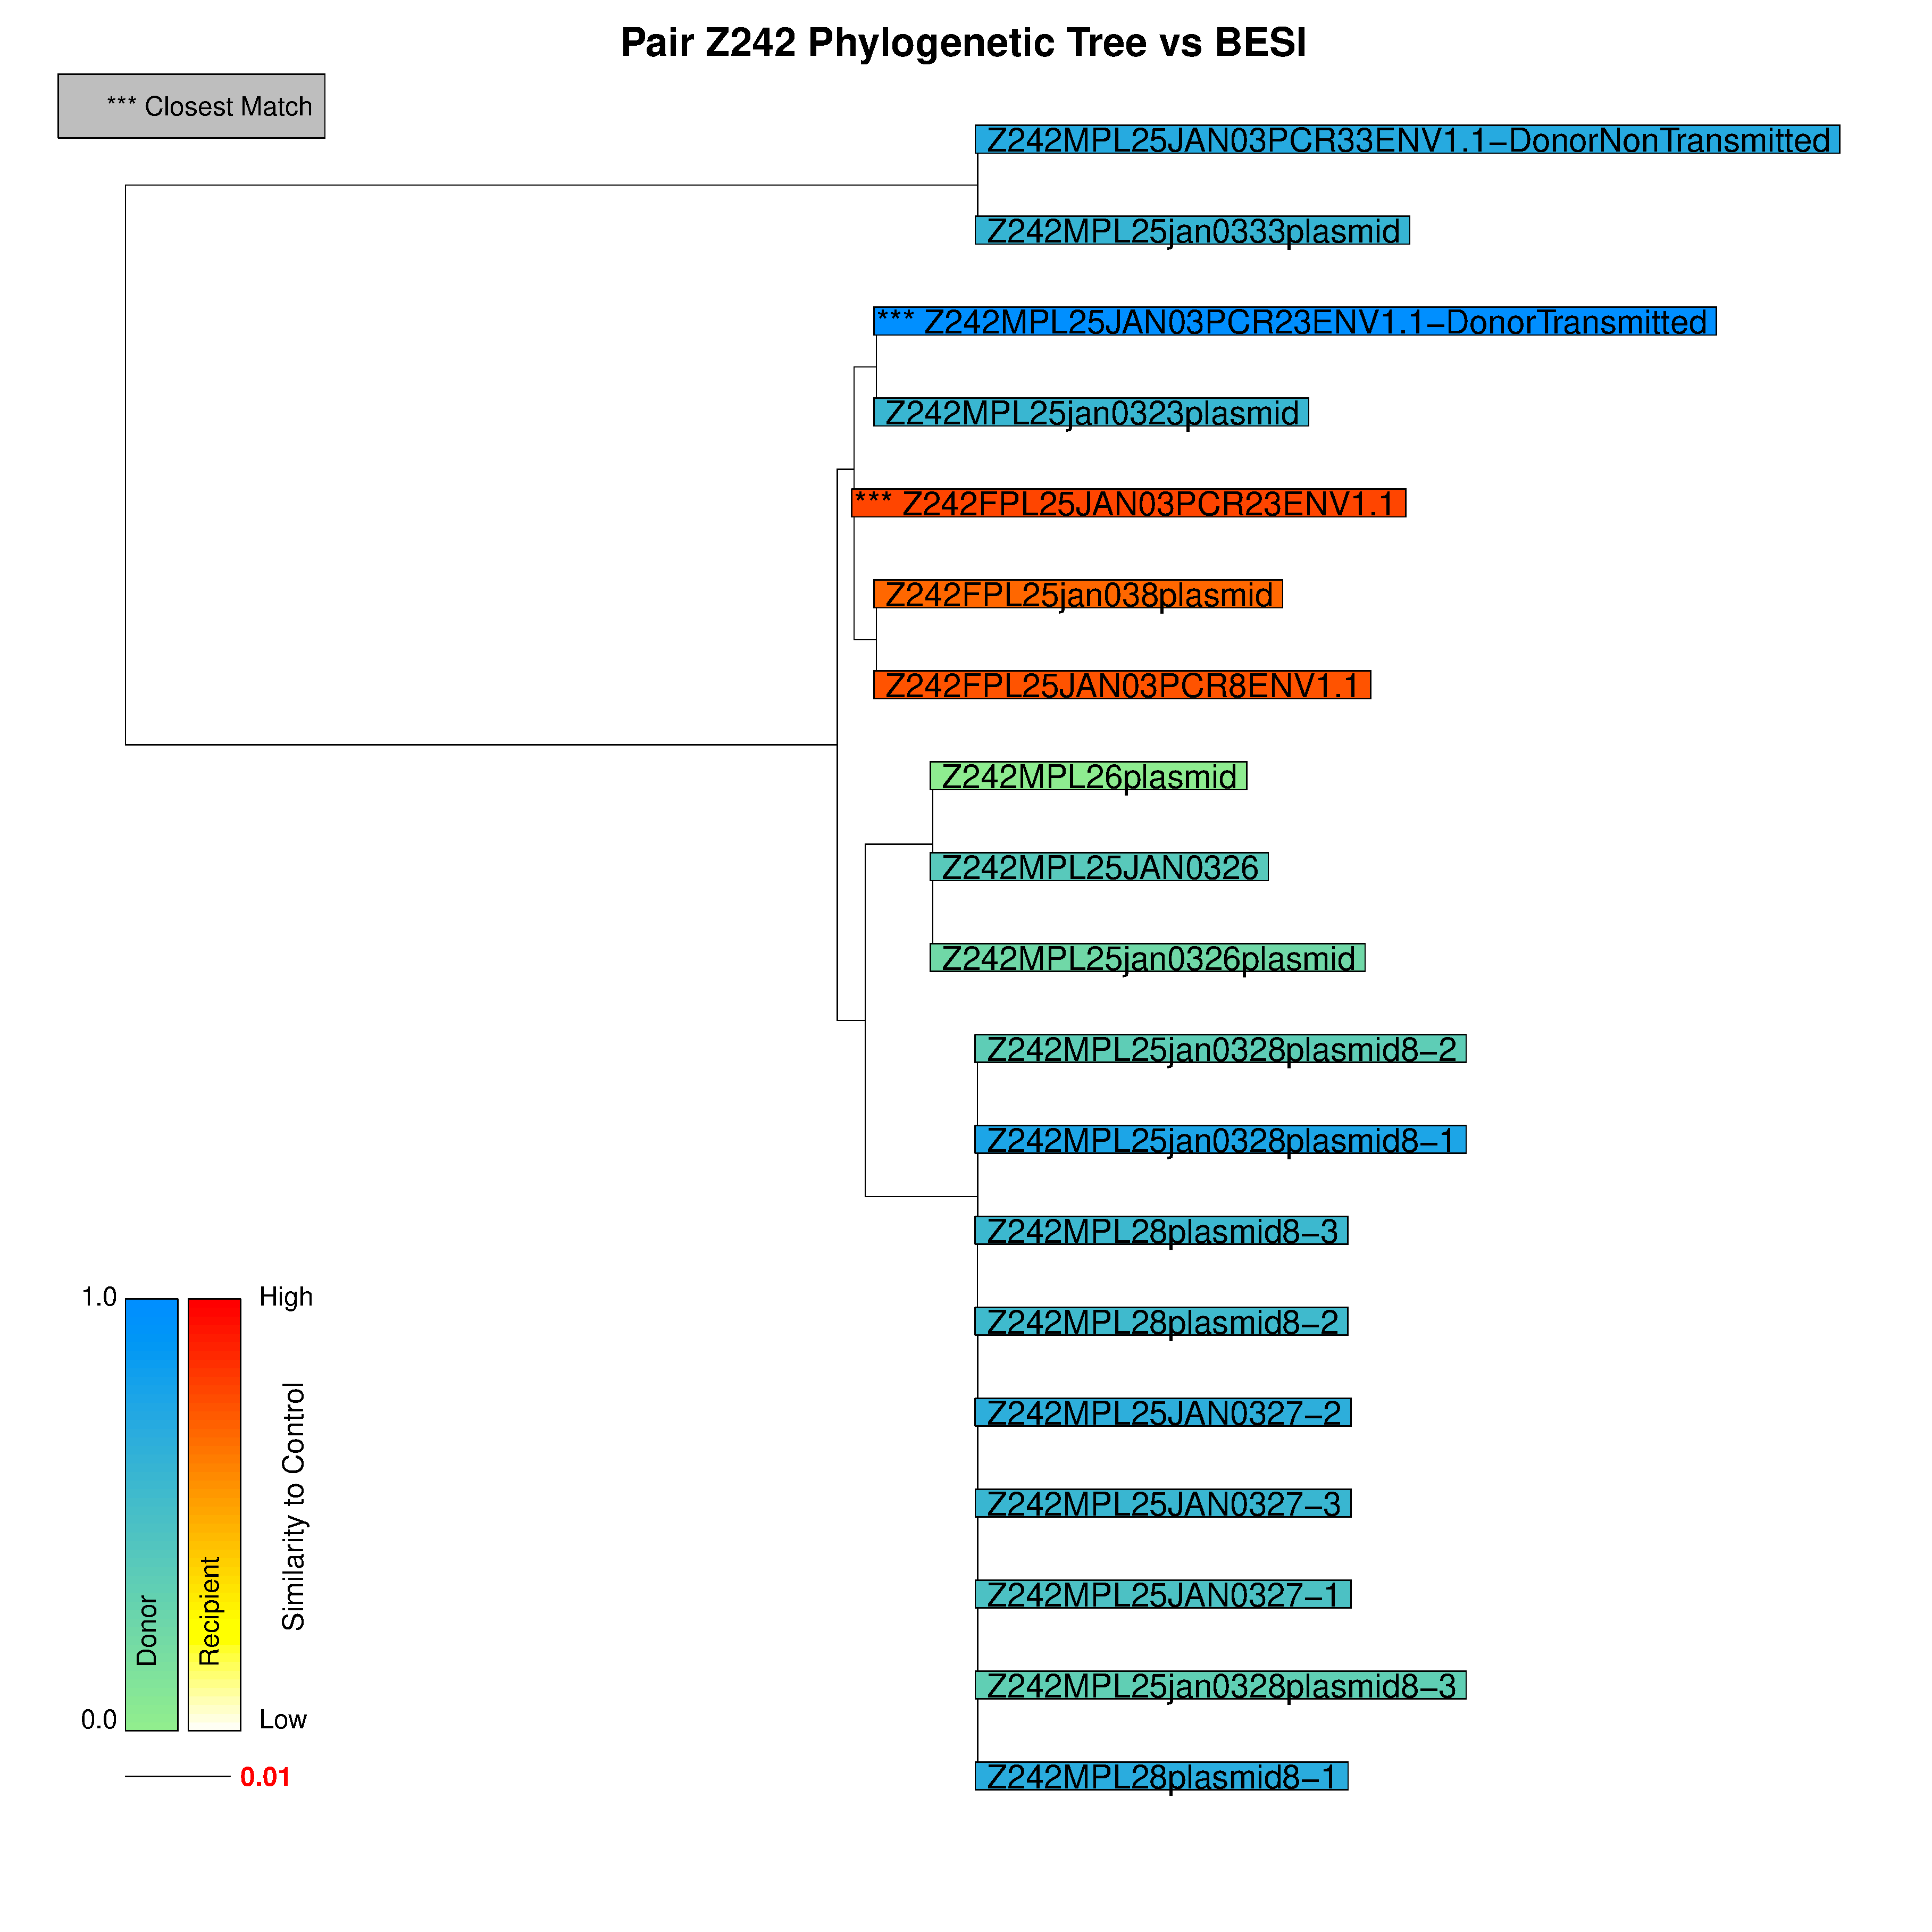
\includegraphics[width=\linewidth]{Z242_heat_map_Fixed-2}} 
\end{minipage}
&	\begin{tabular}{l l l}
	\textbf{Role} & \textbf{Sequence} & \textbf{Score}\\
	\hline
Recipient &	Z242FPL25jan038\_plasmid	&	0.716590787653882	\\
&	Z242FPL25JAN03PCR8ENV1.1	&	0.767818252888392	\\
&	Z242FPL25JAN03PCR23ENV1.1	&	0.807498790248519	\\

	& \ &\ \\
	\hline
Donor &	Z242MPL26\_plasmid	&	0.056761693354295	\\
&	Z242MPL25jan0326\_plasmid	&	0.254514873817641	\\
&	Z242MPL25jan0328\_plasmid\_8-3	&	0.356211803885494	\\
&	Z242MPL25jan0328\_plasmid\_8-2	&	0.364388795656248	\\
&	Z242MPL25JAN0326	&	0.405550291019817	\\
&	Z242MPL25JAN0327-1	&	0.484236134184885	\\
&	Z242MPL28\_plasmid\_8-2	&	0.566663896825258	\\
&	Z242MPL28\_plasmid\_8-3	&	0.586747434644326	\\
&	Z242MPL25JAN0327-3	&	0.607744811003339	\\
&	Z242MPL25jan0323\_plasmid	&	0.616055583249483	\\
&	Z242MPL25jan0333\_plasmid	&	0.634506813877992	\\
&	Z242MPL25JAN0327-2	&	0.696050331698648	\\
&	Z242MPL28\_plasmid\_8-1	&	0.718039064076923	\\
&	Z242MPL25JAN03PCR33ENV1.1-\_Donor\_Non\_Transmitted	&	0.725563289189869	\\
&	Z242MPL25jan0328\_plasmid\_8-1	&	0.781795169546301	\\
&	Z242MPL25JAN03PCR23ENV1.1-\_Donor\_Transmitted	&	1	\\

\end{tabular}\\
\hline
& \ \\
\begin{minipage}{.4\textwidth}
	\raisebox{-\totalheight}{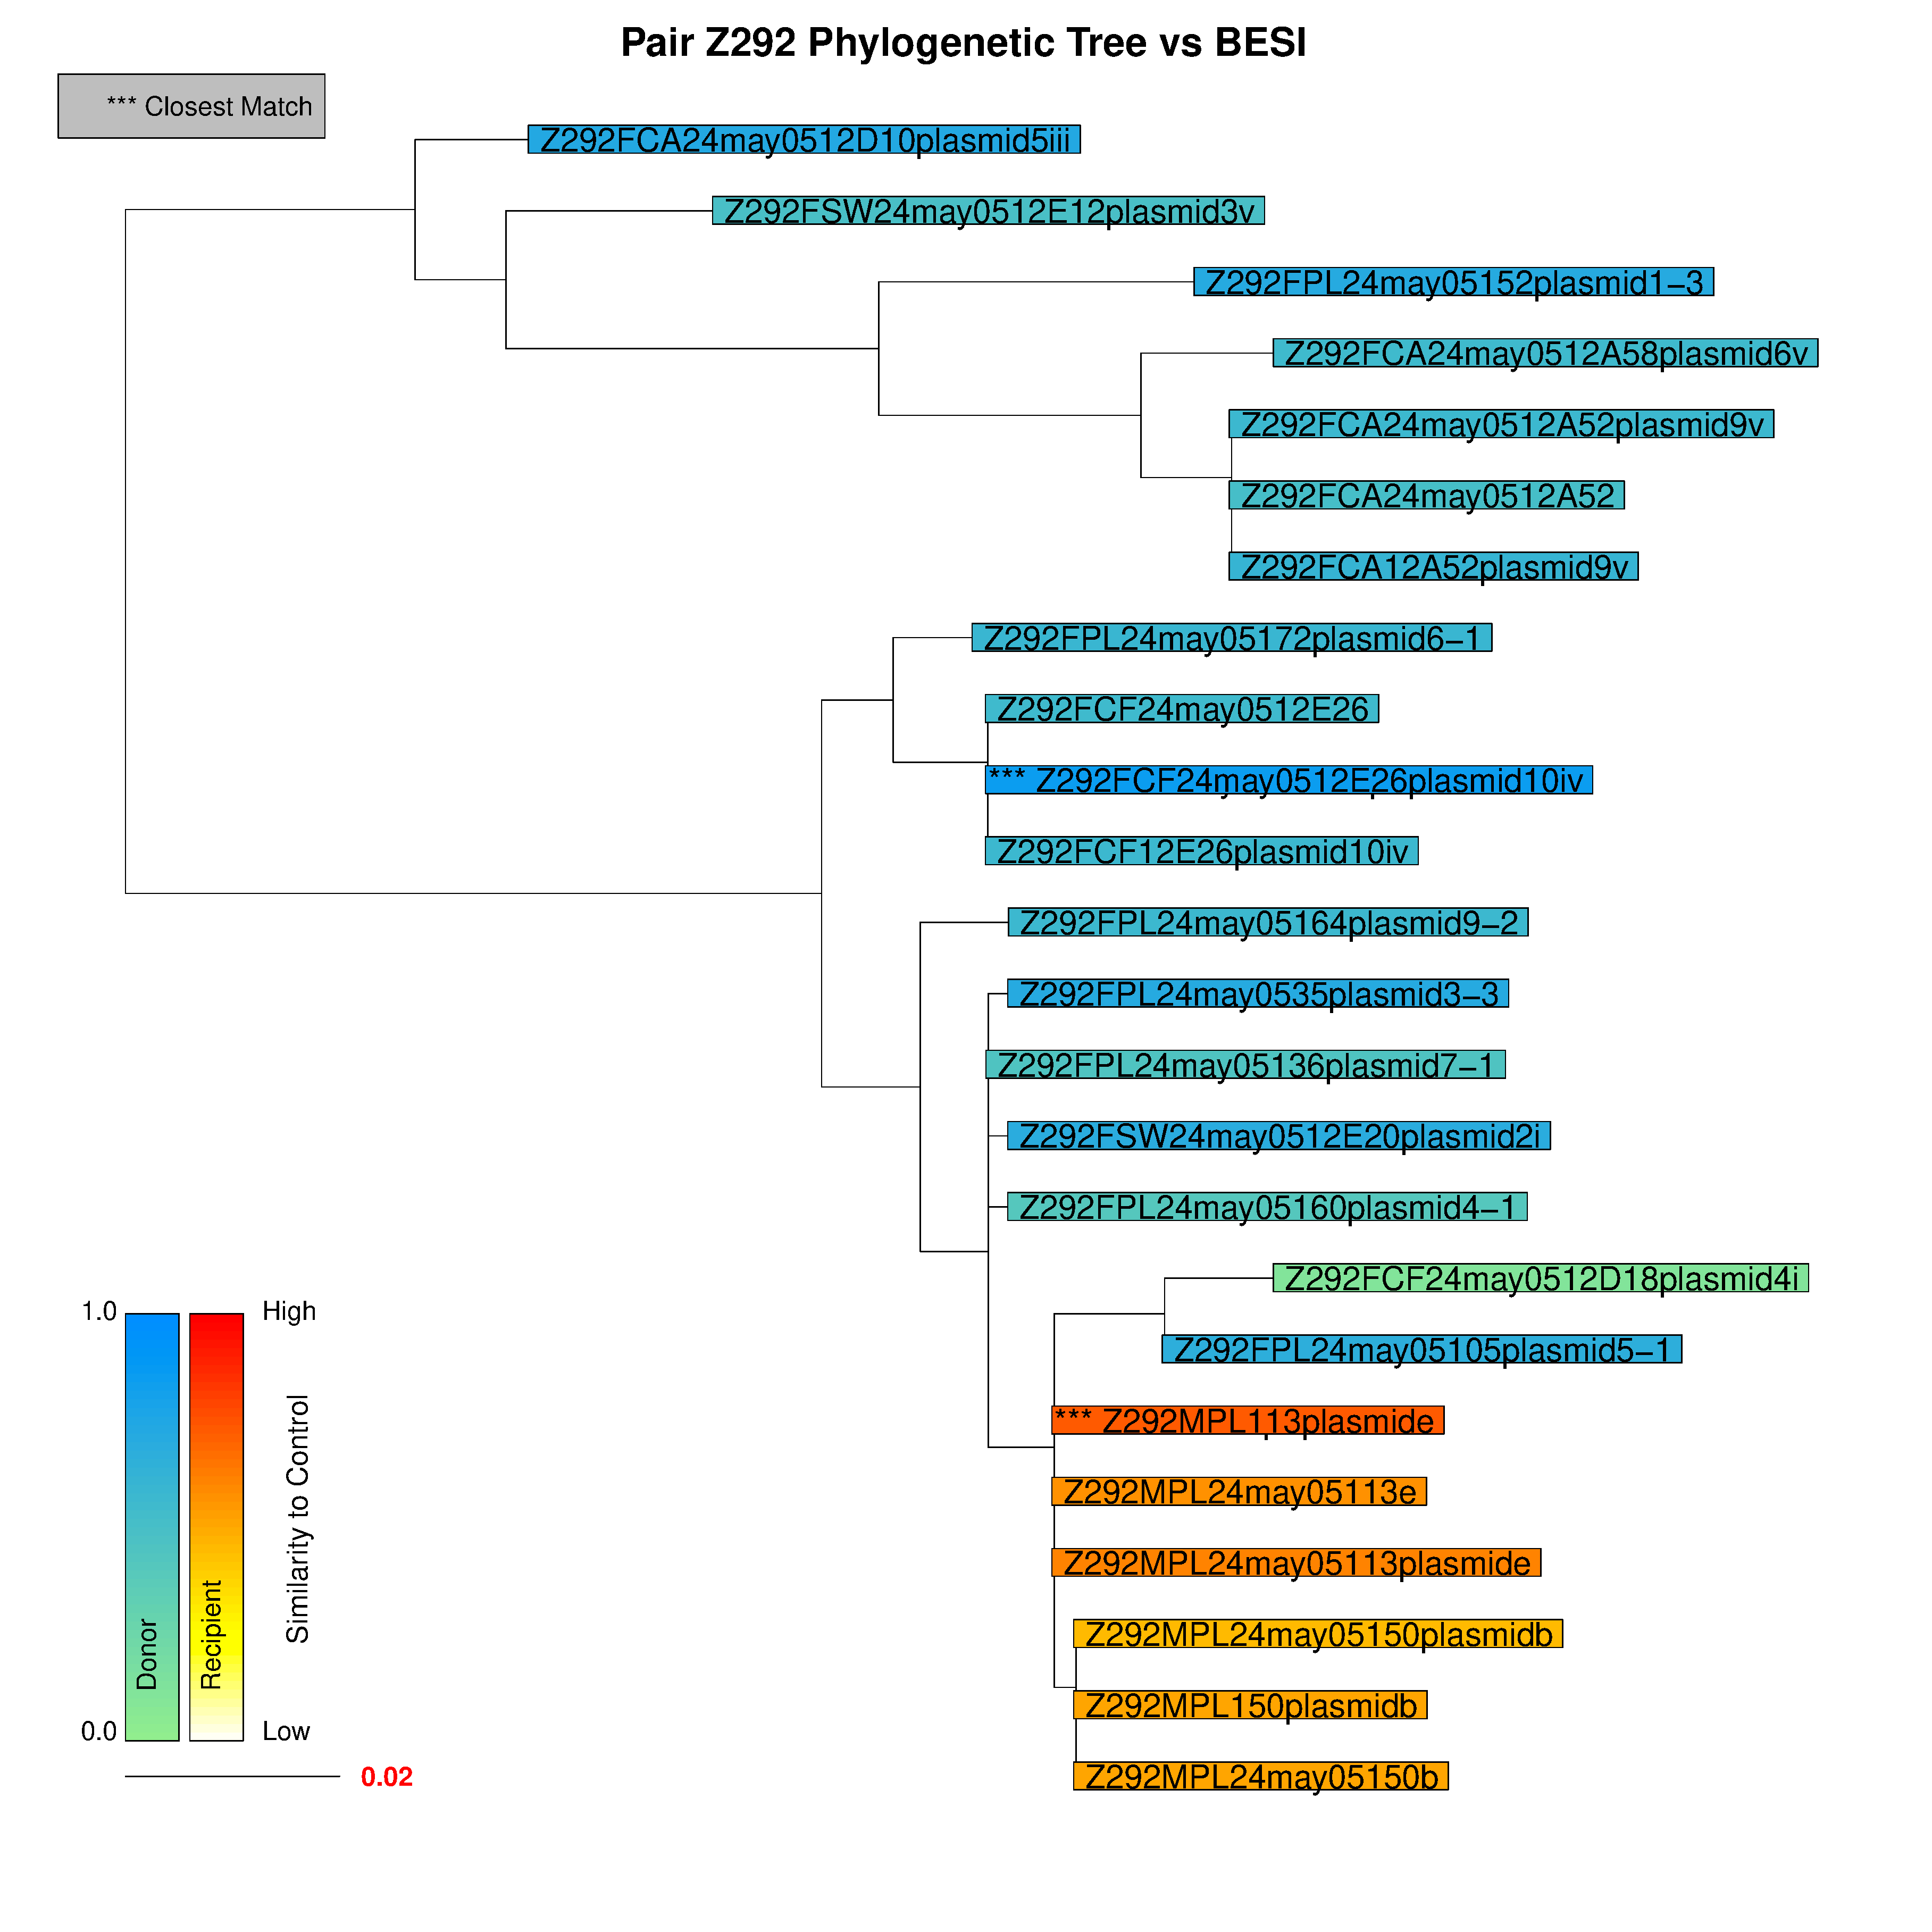
\includegraphics[width=\linewidth]{Z292_heat_map_Fixed-2}} 
\end{minipage}
&	\begin{tabular}{l l l}
	\textbf{Role} & \textbf{Sequence} & \textbf{Score}\\
	\hline
Donor &	Z292FCF24may0512D18\_plasmid\_4i	&	0.137851938524118	\\
&	Z292FPL24may05160\_plasmid\_4-1	&	0.423418833820298	\\
&	Z292FPL24may05136\_plasmid\_7-1	&	0.462179296679748	\\
&	Z292FSW24may0512E12\_plasmid\_3v	&	0.507618540141125	\\
&	Z292FCA24may0512A52	&	0.537991259868594	\\
&	Z292FCF24may0512E26	&	0.561788965888271	\\
&	Z292FCA24may0512A58\_plasmid\_6v	&	0.572122476885801	\\
&	Z292FCF12E26\_plasmid\_10iv	&	0.586681960382053	\\
&	Z292FPL24may05164\_plasmid\_9-2	&	0.595792210633664	\\
&	Z292FCA24may0512A52\_plasmid\_9v	&	0.598113613864758	\\
&	Z292FPL24may05172\_plasmid\_6-1	&	0.600358195601748	\\
&	Z292FCA12A52\_plasmid\_9v	&	0.624773579347445	\\
&	Z292FPL24may05105\_plasmid\_5-1	&	0.686030039474333	\\
&	Z292FSW24may0512E20\_plasmid\_2i	&	0.708384474328787	\\
&	Z292FPL24may0535\_plasmid\_3-3	&	0.735458600274505	\\
&	Z292FPL24may05152\_plasmid\_1-3	&	0.739644683445936	\\
&	Z292FCA24may0512D10\_plasmid\_5iii	&	0.743663635955896	\\
&	Z292FCF24may0512E26\_plasmid\_10iv	&	0.870187354349578	\\

	& \ &\ \\
	\hline
Recipient &	Z292MPL24may05150\_plasmid\_b	&	0.466356596785679	\\
&	Z292MPL24may05150b	&	0.525019744593897	\\
&	Z292MPL150\_plasmid\_b	&	0.539659967550328	\\
&	Z292MPL24may05113e	&	0.583385355065491	\\
&	Z292MPL24may05113\_plasmid\_e	&	0.638241614152609	\\
&	Z292MPL113\_plasmid\_e	&	0.744364853399121	\\

\end{tabular}\\
	\end{tabular}
\end{table*}

\end{document}


